
\begin{frame}
\frametitle{A model space}
\begin{minipage}{.46\columnwidth}
     For a dataset $X$ we study the topology of the \emph{union of balls} 
     \[ M_{\epsilon} = \bigcup_{x \in X} B_{\epsilon}(x) \]
     \only<4->{\textbf{Two Issues:}}
     \setlength{\itemindent}{-3em}
     \begin{description}[\itemindent=0pt]
     \item<4->[\textbf{Scale:}] No natural choice of $\epsilon$! 
     \item<5->[\textbf{Conception:}] How to encode $M_\epsilon$ on computer?
    \end{description}
    \only<6->{\textbf{Answer:} Topology}
    \end{minipage}     
\begin{minipage}{0.55\columnwidth}
\hspace{1cm}
\begin{tikzpicture}[scale=.5]
\only<1>{    \node[draw=none, fill=white] at (0, -5.5) {$r = 0$};}
\only<2-4>{    \node[draw=none, fill=white] at (0, -5.5) {$r = .8$};}
\only<5>{    \node[draw=none, fill=white] at (0, -5.5) {$r = .2$};}
\only<6>{    \node[draw=none, fill=white] at (0, -7.5) {$r = \infty$};}
\only<7>{    \node[draw=none, fill=white] at (0, -7.5) {$r = .6$};}
    \foreach[count=\p] \x / \y in \data {
\only<2-4>{	\begin{pgfonlayer}{ball}
        \fill[gray!50,radius= .8 cm] (\x,\y) circle{};
        \end{pgfonlayer}{ball}
        }
      \only<5>{	\begin{pgfonlayer}{ball}
        \fill[gray!50,radius= .2 cm] (\x,\y) circle{};
        \end{pgfonlayer}{ball}
        }
        \only<6>{	\begin{pgfonlayer}{ball}
        \fill[gray!50,radius= 2.4 cm] (\x,\y) circle{};
        \end{pgfonlayer}{ball}
        }
        \only<7>{	\begin{pgfonlayer}{ball}
        \fill[gray!50,radius= .6 cm] (\x,\y) circle{};
        \end{pgfonlayer}{ball}
        }
	\node[draw, circle, scale=.25, fill=white](\p) at (\x, \y) {};
    } 
\end{tikzpicture}
\end{minipage}
\end{frame}

\begin{frame}[fragile]
\frametitle{Simplicial Complexes}
\begin{figure}
\centering
  \includegraphics[width=.6\textwidth]{simplicial}
 \caption{(left) an example \phantom{2000}  (right) a non example}
\end{figure}
For a vertex set $V$ a simplicial complex $K \subseteq 2^V$ satisfying:
\begin{enumerate}
\item $\{ v \} \in K$ for each $v \in V$
\item if $\tau \subseteq \sigma \in K$  then $\tau \in K$. 
\item if $\sigma$ is a $k$-simplex if $\card{\sigma} = k+1$ 
\end{enumerate}
\end{frame}

\begin{frame}{Simplicial Complexes}
\centering
\begin{minipage}{0.45\columnwidth}%
\begin{tikzpicture}[scale=.5]
	\node[draw=none, fill=white] at (0, -5.5) {$\check{C}_{.6}$};
    \foreach[count=\p] \x / \y in \data {
	\begin{pgfonlayer}{ball}
        \fill[gray!50,radius= .6 cm] (\x,\y) circle{};
        \end{pgfonlayer}{ball}
	\node[draw, circle, scale=.25, fill=white](\p) at (\x, \y) {};
    } 

\input{cell_5_nerve}
 \end{tikzpicture}
\end{minipage}%
\begin{minipage}{0.55\columnwidth}%
The $\check{C}$ech complex $\check{C}_{\epsilon}$ encodes the intersection pattern
of $M_{\epsilon}$:
\only<2->{Encode:} 
\begin{itemize}
\item<2->Points as \emph{vertices} (0-cells)
\item<3->Pairwise intersections as \emph{edges} (1-cells)
\item<4->Threeway intersections as \emph{triangles} (2-cells)
\item<5->$k$-way intersections as \emph{(k+1)-cells}
\end{itemize}
\end{minipage}
\only<6->{
\begin{lemma}{Nerve Lemma}[Leray '45]
$\check{C}_\epsilon$ is topologically equivalent to $M_\epsilon$.
\end{lemma}
}
\end{frame}

\begin{frame}
\frametitle{Which $\epsilon$? Don't settle for parameter choices}
\begin{minipage}{0.45\columnwidth}%
\begin{tikzpicture}[scale=.5]
 \node[draw=none, fill=white] at (0, -5.5) {$\check{C}_{.6}$};
    \foreach[count=\p] \x / \y in \data {
	\begin{pgfonlayer}{ball}
        \fill[gray!50,radius= .6 cm] (\x,\y) circle{};
        \end{pgfonlayer}{ball}
	\node[draw, circle, scale=.25, fill=white](\p) at (\x, \y) {};
    } 
 \begin{pgfonlayer}{edge} 
\draw (1) -- (6); 
\draw (1) -- (12); 
\draw (1) -- (19); 
\draw (1) -- (23); 
\draw (1) -- (26); 
\draw (1) -- (48); 
\draw (1) -- (50); 
\draw (1) -- (57); 
\draw (1) -- (68); 
\draw (1) -- (71); 
\draw (1) -- (96); 
\draw (1) -- (98); 
\draw (2) -- (8); 
\draw (2) -- (35); 
\draw (2) -- (47); 
\draw (2) -- (58); 
\draw (2) -- (64); 
\draw (2) -- (89); 
\draw (2) -- (97); 
\draw (3) -- (29); 
\draw (3) -- (39); 
\draw (3) -- (40); 
\draw (3) -- (51); 
\draw (3) -- (65); 
\draw (3) -- (73); 
\draw (3) -- (81); 
\draw (3) -- (91); 
\draw (3) -- (94); 
\draw (4) -- (59); 
\draw (4) -- (70); 
\draw (4) -- (85); 
\draw (4) -- (86); 
\draw (4) -- (88); 
\draw (4) -- (99); 
\draw (4) -- (102); 
\draw (5) -- (24); 
\draw (5) -- (54); 
\draw (5) -- (58); 
\draw (5) -- (63); 
\draw (5) -- (64); 
\draw (5) -- (100); 
\draw (6) -- (19); 
\draw (6) -- (26); 
\draw (6) -- (48); 
\draw (6) -- (57); 
\draw (6) -- (68); 
\draw (6) -- (71); 
\draw (6) -- (98); 
\draw (7) -- (15); 
\draw (7) -- (21); 
\draw (7) -- (39); 
\draw (7) -- (53); 
\draw (7) -- (81); 
\draw (8) -- (18); 
\draw (8) -- (24); 
\draw (8) -- (35); 
\draw (8) -- (54); 
\draw (8) -- (55); 
\draw (8) -- (63); 
\draw (8) -- (64); 
\draw (8) -- (89); 
\draw (9) -- (12); 
\draw (9) -- (23); 
\draw (9) -- (26); 
\draw (9) -- (28); 
\draw (9) -- (32); 
\draw (9) -- (50); 
\draw (9) -- (56); 
\draw (9) -- (67); 
\draw (9) -- (96); 
\draw (10) -- (29); 
\draw (10) -- (40); 
\draw (10) -- (49); 
\draw (10) -- (52); 
\draw (10) -- (65); 
\draw (10) -- (69); 
\draw (10) -- (77); 
\draw (10) -- (78); 
\draw (10) -- (80); 
\draw (10) -- (83); 
\draw (11) -- (13); 
\draw (11) -- (20); 
\draw (11) -- (33); 
\draw (11) -- (41); 
\draw (11) -- (44); 
\draw (11) -- (45); 
\draw (11) -- (46); 
\draw (11) -- (72); 
\draw (11) -- (90); 
\draw (11) -- (93); 
\draw (11) -- (95); 
\draw (12) -- (23); 
\draw (12) -- (25); 
\draw (12) -- (26); 
\draw (12) -- (28); 
\draw (12) -- (32); 
\draw (12) -- (50); 
\draw (12) -- (67); 
\draw (12) -- (68); 
\draw (12) -- (87); 
\draw (12) -- (96); 
\draw (12) -- (98); 
\draw (13) -- (20); 
\draw (13) -- (44); 
\draw (13) -- (61); 
\draw (13) -- (72); 
\draw (13) -- (82); 
\draw (13) -- (90); 
\draw (13) -- (95); 
\draw (14) -- (30); 
\draw (14) -- (31); 
\draw (14) -- (34); 
\draw (14) -- (43); 
\draw (14) -- (55); 
\draw (14) -- (60); 
\draw (14) -- (75); 
\draw (14) -- (76); 
\draw (14) -- (84); 
\draw (14) -- (92); 
\draw (15) -- (21); 
\draw (15) -- (39); 
\draw (15) -- (51); 
\draw (15) -- (53); 
\draw (15) -- (65); 
\draw (15) -- (73); 
\draw (15) -- (81); 
\draw (16) -- (17); 
\draw (16) -- (19); 
\draw (16) -- (38); 
\draw (16) -- (57); 
\draw (16) -- (62); 
\draw (16) -- (79); 
\draw (17) -- (22); 
\draw (17) -- (38); 
\draw (17) -- (57); 
\draw (17) -- (62); 
\draw (17) -- (74); 
\draw (17) -- (79); 
\draw (18) -- (35); 
\draw (18) -- (54); 
\draw (18) -- (55); 
\draw (18) -- (63); 
\draw (18) -- (64); 
\draw (18) -- (76); 
\draw (18) -- (89); 
\draw (19) -- (48); 
\draw (19) -- (57); 
\draw (19) -- (71); 
\draw (19) -- (79); 
\draw (20) -- (41); 
\draw (20) -- (44); 
\draw (20) -- (45); 
\draw (20) -- (46); 
\draw (20) -- (72); 
\draw (20) -- (82); 
\draw (20) -- (90); 
\draw (20) -- (93); 
\draw (20) -- (95); 
\draw (21) -- (39); 
\draw (21) -- (53); 
\draw (21) -- (81); 
\draw (21) -- (91); 
\draw (21) -- (94); 
\draw (21) -- (100); 
\draw (22) -- (70); 
\draw (22) -- (74); 
\draw (22) -- (85); 
\draw (22) -- (88); 
\draw (22) -- (99); 
\draw (23) -- (26); 
\draw (23) -- (28); 
\draw (23) -- (32); 
\draw (23) -- (50); 
\draw (23) -- (56); 
\draw (23) -- (67); 
\draw (23) -- (68); 
\draw (23) -- (87); 
\draw (23) -- (96); 
\draw (23) -- (98); 
\draw (24) -- (54); 
\draw (24) -- (58); 
\draw (24) -- (63); 
\draw (24) -- (64); 
\draw (25) -- (28); 
\draw (25) -- (32); 
\draw (25) -- (66); 
\draw (25) -- (67); 
\draw (25) -- (68); 
\draw (25) -- (87); 
\draw (25) -- (96); 
\draw (25) -- (98); 
\draw (26) -- (32); 
\draw (26) -- (50); 
\draw (26) -- (67); 
\draw (26) -- (68); 
\draw (26) -- (96); 
\draw (26) -- (98); 
\draw (27) -- (36); 
\draw (27) -- (37); 
\draw (27) -- (56); 
\draw (27) -- (101); 
\draw (28) -- (32); 
\draw (28) -- (37); 
\draw (28) -- (56); 
\draw (28) -- (66); 
\draw (28) -- (67); 
\draw (28) -- (87); 
\draw (28) -- (96); 
\draw (28) -- (101); 
\draw (29) -- (40); 
\draw (29) -- (51); 
\draw (29) -- (52); 
\draw (29) -- (65); 
\draw (29) -- (73); 
\draw (29) -- (77); 
\draw (29) -- (78); 
\draw (29) -- (80); 
\draw (29) -- (83); 
\draw (30) -- (31); 
\draw (30) -- (34); 
\draw (30) -- (43); 
\draw (30) -- (55); 
\draw (30) -- (60); 
\draw (30) -- (75); 
\draw (30) -- (76); 
\draw (30) -- (84); 
\draw (30) -- (92); 
\draw (31) -- (43); 
\draw (31) -- (55); 
\draw (31) -- (60); 
\draw (31) -- (75); 
\draw (31) -- (76); 
\draw (31) -- (84); 
\draw (31) -- (92); 
\draw (32) -- (50); 
\draw (32) -- (56); 
\draw (32) -- (67); 
\draw (32) -- (68); 
\draw (32) -- (87); 
\draw (32) -- (96); 
\draw (32) -- (98); 
\draw (33) -- (41); 
\draw (33) -- (46); 
\draw (33) -- (86); 
\draw (33) -- (93); 
\draw (34) -- (36); 
\draw (34) -- (37); 
\draw (34) -- (43); 
\draw (34) -- (60); 
\draw (34) -- (66); 
\draw (34) -- (75); 
\draw (34) -- (84); 
\draw (34) -- (92); 
\draw (35) -- (47); 
\draw (35) -- (55); 
\draw (35) -- (64); 
\draw (35) -- (76); 
\draw (35) -- (89); 
\draw (36) -- (37); 
\draw (36) -- (66); 
\draw (36) -- (84); 
\draw (36) -- (101); 
\draw (37) -- (56); 
\draw (37) -- (66); 
\draw (37) -- (101); 
\draw (38) -- (62); 
\draw (38) -- (74); 
\draw (39) -- (73); 
\draw (39) -- (81); 
\draw (39) -- (91); 
\draw (39) -- (94); 
\draw (40) -- (42); 
\draw (40) -- (49); 
\draw (40) -- (52); 
\draw (40) -- (73); 
\draw (40) -- (77); 
\draw (40) -- (78); 
\draw (40) -- (80); 
\draw (40) -- (83); 
\draw (41) -- (44); 
\draw (41) -- (45); 
\draw (41) -- (46); 
\draw (41) -- (72); 
\draw (41) -- (90); 
\draw (41) -- (93); 
\draw (41) -- (95); 
\draw (41) -- (102); 
\draw (42) -- (44); 
\draw (42) -- (49); 
\draw (42) -- (61); 
\draw (42) -- (69); 
\draw (42) -- (77); 
\draw (42) -- (78); 
\draw (42) -- (80); 
\draw (42) -- (82); 
\draw (42) -- (90); 
\draw (42) -- (95); 
\draw (43) -- (60); 
\draw (43) -- (75); 
\draw (43) -- (76); 
\draw (43) -- (84); 
\draw (43) -- (92); 
\draw (44) -- (45); 
\draw (44) -- (46); 
\draw (44) -- (49); 
\draw (44) -- (72); 
\draw (44) -- (82); 
\draw (44) -- (90); 
\draw (44) -- (93); 
\draw (44) -- (95); 
\draw (45) -- (46); 
\draw (45) -- (72); 
\draw (45) -- (82); 
\draw (45) -- (90); 
\draw (45) -- (93); 
\draw (45) -- (95); 
\draw (45) -- (102); 
\draw (46) -- (72); 
\draw (46) -- (90); 
\draw (46) -- (93); 
\draw (46) -- (95); 
\draw (46) -- (102); 
\draw (47) -- (55); 
\draw (47) -- (60); 
\draw (47) -- (89); 
\draw (48) -- (57); 
\draw (48) -- (68); 
\draw (48) -- (71); 
\draw (48) -- (79); 
\draw (48) -- (96); 
\draw (48) -- (98); 
\draw (49) -- (61); 
\draw (49) -- (69); 
\draw (49) -- (77); 
\draw (49) -- (78); 
\draw (49) -- (80); 
\draw (49) -- (82); 
\draw (49) -- (83); 
\draw (49) -- (90); 
\draw (49) -- (95); 
\draw (50) -- (67); 
\draw (50) -- (68); 
\draw (50) -- (96); 
\draw (50) -- (98); 
\draw (51) -- (52); 
\draw (51) -- (65); 
\draw (51) -- (73); 
\draw (52) -- (65); 
\draw (52) -- (73); 
\draw (52) -- (77); 
\draw (52) -- (78); 
\draw (52) -- (80); 
\draw (52) -- (83); 
\draw (53) -- (81); 
\draw (53) -- (100); 
\draw (54) -- (63); 
\draw (54) -- (64); 
\draw (55) -- (60); 
\draw (55) -- (75); 
\draw (55) -- (76); 
\draw (55) -- (89); 
\draw (55) -- (92); 
\draw (56) -- (67); 
\draw (56) -- (101); 
\draw (57) -- (71); 
\draw (57) -- (79); 
\draw (58) -- (64); 
\draw (58) -- (97); 
\draw (58) -- (100); 
\draw (59) -- (70); 
\draw (59) -- (85); 
\draw (59) -- (86); 
\draw (59) -- (88); 
\draw (59) -- (99); 
\draw (60) -- (75); 
\draw (60) -- (76); 
\draw (60) -- (84); 
\draw (60) -- (92); 
\draw (61) -- (69); 
\draw (61) -- (77); 
\draw (61) -- (78); 
\draw (61) -- (80); 
\draw (61) -- (82); 
\draw (61) -- (90); 
\draw (61) -- (95); 
\draw (62) -- (74); 
\draw (62) -- (79); 
\draw (63) -- (64); 
\draw (64) -- (89); 
\draw (65) -- (73); 
\draw (65) -- (83); 
\draw (66) -- (87); 
\draw (67) -- (68); 
\draw (67) -- (87); 
\draw (67) -- (96); 
\draw (67) -- (98); 
\draw (68) -- (71); 
\draw (68) -- (87); 
\draw (68) -- (96); 
\draw (68) -- (98); 
\draw (69) -- (77); 
\draw (69) -- (78); 
\draw (69) -- (80); 
\draw (69) -- (82); 
\draw (69) -- (83); 
\draw (69) -- (95); 
\draw (70) -- (74); 
\draw (70) -- (85); 
\draw (70) -- (88); 
\draw (70) -- (99); 
\draw (71) -- (79); 
\draw (71) -- (98); 
\draw (72) -- (82); 
\draw (72) -- (90); 
\draw (72) -- (93); 
\draw (72) -- (95); 
\draw (73) -- (81); 
\draw (73) -- (91); 
\draw (73) -- (94); 
\draw (74) -- (85); 
\draw (74) -- (88); 
\draw (75) -- (76); 
\draw (75) -- (84); 
\draw (75) -- (92); 
\draw (76) -- (84); 
\draw (76) -- (89); 
\draw (76) -- (92); 
\draw (77) -- (78); 
\draw (77) -- (80); 
\draw (77) -- (82); 
\draw (77) -- (83); 
\draw (78) -- (80); 
\draw (78) -- (83); 
\draw (80) -- (82); 
\draw (80) -- (83); 
\draw (81) -- (91); 
\draw (81) -- (94); 
\draw (82) -- (90); 
\draw (82) -- (93); 
\draw (82) -- (95); 
\draw (84) -- (92); 
\draw (85) -- (86); 
\draw (85) -- (88); 
\draw (85) -- (99); 
\draw (86) -- (99); 
\draw (87) -- (96); 
\draw (87) -- (98); 
\draw (88) -- (99); 
\draw (89) -- (92); 
\draw (90) -- (93); 
\draw (90) -- (95); 
\draw (91) -- (94); 
\draw (91) -- (97); 
\draw (93) -- (95); 
\draw (93) -- (102); 
\draw (96) -- (98); 
\end{pgfonlayer}{edge} 
\begin{pgfonlayer}{triangle} 
\fill[complex_triangle] (1.center) -- (19.center) -- (6.center) -- cycle; 
\fill[complex_triangle] (1.center) -- (26.center) -- (6.center) -- cycle; 
\fill[complex_triangle] (48.center) -- (1.center) -- (6.center) -- cycle; 
\fill[complex_triangle] (1.center) -- (6.center) -- (57.center) -- cycle; 
\fill[complex_triangle] (1.center) -- (68.center) -- (6.center) -- cycle; 
\fill[complex_triangle] (1.center) -- (6.center) -- (71.center) -- cycle; 
\fill[complex_triangle] (1.center) -- (98.center) -- (6.center) -- cycle; 
\fill[complex_triangle] (1.center) -- (12.center) -- (23.center) -- cycle; 
\fill[complex_triangle] (1.center) -- (26.center) -- (12.center) -- cycle; 
\fill[complex_triangle] (1.center) -- (50.center) -- (12.center) -- cycle; 
\fill[complex_triangle] (68.center) -- (1.center) -- (12.center) -- cycle; 
\fill[complex_triangle] (96.center) -- (1.center) -- (12.center) -- cycle; 
\fill[complex_triangle] (1.center) -- (98.center) -- (12.center) -- cycle; 
\fill[complex_triangle] (48.center) -- (1.center) -- (19.center) -- cycle; 
\fill[complex_triangle] (1.center) -- (19.center) -- (57.center) -- cycle; 
\fill[complex_triangle] (1.center) -- (19.center) -- (71.center) -- cycle; 
\fill[complex_triangle] (1.center) -- (26.center) -- (23.center) -- cycle; 
\fill[complex_triangle] (1.center) -- (50.center) -- (23.center) -- cycle; 
\fill[complex_triangle] (1.center) -- (68.center) -- (23.center) -- cycle; 
\fill[complex_triangle] (96.center) -- (1.center) -- (23.center) -- cycle; 
\fill[complex_triangle] (1.center) -- (98.center) -- (23.center) -- cycle; 
\fill[complex_triangle] (1.center) -- (26.center) -- (50.center) -- cycle; 
\fill[complex_triangle] (1.center) -- (26.center) -- (68.center) -- cycle; 
\fill[complex_triangle] (96.center) -- (1.center) -- (26.center) -- cycle; 
\fill[complex_triangle] (1.center) -- (26.center) -- (98.center) -- cycle; 
\fill[complex_triangle] (48.center) -- (1.center) -- (57.center) -- cycle; 
\fill[complex_triangle] (48.center) -- (1.center) -- (68.center) -- cycle; 
\fill[complex_triangle] (48.center) -- (1.center) -- (71.center) -- cycle; 
\fill[complex_triangle] (48.center) -- (1.center) -- (96.center) -- cycle; 
\fill[complex_triangle] (48.center) -- (1.center) -- (98.center) -- cycle; 
\fill[complex_triangle] (1.center) -- (50.center) -- (68.center) -- cycle; 
\fill[complex_triangle] (96.center) -- (1.center) -- (50.center) -- cycle; 
\fill[complex_triangle] (1.center) -- (50.center) -- (98.center) -- cycle; 
\fill[complex_triangle] (1.center) -- (71.center) -- (57.center) -- cycle; 
\fill[complex_triangle] (1.center) -- (68.center) -- (71.center) -- cycle; 
\fill[complex_triangle] (96.center) -- (1.center) -- (68.center) -- cycle; 
\fill[complex_triangle] (1.center) -- (98.center) -- (68.center) -- cycle; 
\fill[complex_triangle] (1.center) -- (98.center) -- (71.center) -- cycle; 
\fill[complex_triangle] (96.center) -- (1.center) -- (98.center) -- cycle; 
\fill[complex_triangle] (8.center) -- (2.center) -- (35.center) -- cycle; 
\fill[complex_triangle] (8.center) -- (64.center) -- (2.center) -- cycle; 
\fill[complex_triangle] (8.center) -- (89.center) -- (2.center) -- cycle; 
\fill[complex_triangle] (2.center) -- (35.center) -- (47.center) -- cycle; 
\fill[complex_triangle] (64.center) -- (2.center) -- (35.center) -- cycle; 
\fill[complex_triangle] (89.center) -- (2.center) -- (35.center) -- cycle; 
\fill[complex_triangle] (89.center) -- (2.center) -- (47.center) -- cycle; 
\fill[complex_triangle] (64.center) -- (2.center) -- (58.center) -- cycle; 
\fill[complex_triangle] (97.center) -- (2.center) -- (58.center) -- cycle; 
\fill[complex_triangle] (64.center) -- (89.center) -- (2.center) -- cycle; 
\fill[complex_triangle] (40.center) -- (3.center) -- (29.center) -- cycle; 
\fill[complex_triangle] (51.center) -- (3.center) -- (29.center) -- cycle; 
\fill[complex_triangle] (65.center) -- (3.center) -- (29.center) -- cycle; 
\fill[complex_triangle] (73.center) -- (3.center) -- (29.center) -- cycle; 
\fill[complex_triangle] (73.center) -- (3.center) -- (39.center) -- cycle; 
\fill[complex_triangle] (81.center) -- (3.center) -- (39.center) -- cycle; 
\fill[complex_triangle] (91.center) -- (3.center) -- (39.center) -- cycle; 
\fill[complex_triangle] (3.center) -- (94.center) -- (39.center) -- cycle; 
\fill[complex_triangle] (40.center) -- (73.center) -- (3.center) -- cycle; 
\fill[complex_triangle] (51.center) -- (3.center) -- (65.center) -- cycle; 
\fill[complex_triangle] (51.center) -- (3.center) -- (73.center) -- cycle; 
\fill[complex_triangle] (65.center) -- (3.center) -- (73.center) -- cycle; 
\fill[complex_triangle] (73.center) -- (3.center) -- (81.center) -- cycle; 
\fill[complex_triangle] (73.center) -- (91.center) -- (3.center) -- cycle; 
\fill[complex_triangle] (73.center) -- (3.center) -- (94.center) -- cycle; 
\fill[complex_triangle] (81.center) -- (91.center) -- (3.center) -- cycle; 
\fill[complex_triangle] (81.center) -- (3.center) -- (94.center) -- cycle; 
\fill[complex_triangle] (91.center) -- (3.center) -- (94.center) -- cycle; 
\fill[complex_triangle] (59.center) -- (4.center) -- (70.center) -- cycle; 
\fill[complex_triangle] (59.center) -- (4.center) -- (85.center) -- cycle; 
\fill[complex_triangle] (59.center) -- (4.center) -- (86.center) -- cycle; 
\fill[complex_triangle] (88.center) -- (59.center) -- (4.center) -- cycle; 
\fill[complex_triangle] (99.center) -- (59.center) -- (4.center) -- cycle; 
\fill[complex_triangle] (4.center) -- (85.center) -- (70.center) -- cycle; 
\fill[complex_triangle] (88.center) -- (4.center) -- (70.center) -- cycle; 
\fill[complex_triangle] (99.center) -- (4.center) -- (70.center) -- cycle; 
\fill[complex_triangle] (4.center) -- (85.center) -- (86.center) -- cycle; 
\fill[complex_triangle] (88.center) -- (4.center) -- (85.center) -- cycle; 
\fill[complex_triangle] (99.center) -- (4.center) -- (85.center) -- cycle; 
\fill[complex_triangle] (99.center) -- (4.center) -- (86.center) -- cycle; 
\fill[complex_triangle] (88.center) -- (99.center) -- (4.center) -- cycle; 
\fill[complex_triangle] (24.center) -- (5.center) -- (54.center) -- cycle; 
\fill[complex_triangle] (24.center) -- (58.center) -- (5.center) -- cycle; 
\fill[complex_triangle] (24.center) -- (5.center) -- (63.center) -- cycle; 
\fill[complex_triangle] (24.center) -- (64.center) -- (5.center) -- cycle; 
\fill[complex_triangle] (5.center) -- (54.center) -- (63.center) -- cycle; 
\fill[complex_triangle] (64.center) -- (5.center) -- (54.center) -- cycle; 
\fill[complex_triangle] (64.center) -- (58.center) -- (5.center) -- cycle; 
\fill[complex_triangle] (58.center) -- (100.center) -- (5.center) -- cycle; 
\fill[complex_triangle] (64.center) -- (5.center) -- (63.center) -- cycle; 
\fill[complex_triangle] (48.center) -- (19.center) -- (6.center) -- cycle; 
\fill[complex_triangle] (57.center) -- (19.center) -- (6.center) -- cycle; 
\fill[complex_triangle] (19.center) -- (6.center) -- (71.center) -- cycle; 
\fill[complex_triangle] (26.center) -- (68.center) -- (6.center) -- cycle; 
\fill[complex_triangle] (26.center) -- (98.center) -- (6.center) -- cycle; 
\fill[complex_triangle] (48.center) -- (57.center) -- (6.center) -- cycle; 
\fill[complex_triangle] (48.center) -- (68.center) -- (6.center) -- cycle; 
\fill[complex_triangle] (48.center) -- (6.center) -- (71.center) -- cycle; 
\fill[complex_triangle] (48.center) -- (98.center) -- (6.center) -- cycle; 
\fill[complex_triangle] (57.center) -- (6.center) -- (71.center) -- cycle; 
\fill[complex_triangle] (68.center) -- (6.center) -- (71.center) -- cycle; 
\fill[complex_triangle] (98.center) -- (68.center) -- (6.center) -- cycle; 
\fill[complex_triangle] (98.center) -- (6.center) -- (71.center) -- cycle; 
\fill[complex_triangle] (15.center) -- (21.center) -- (7.center) -- cycle; 
\fill[complex_triangle] (39.center) -- (15.center) -- (7.center) -- cycle; 
\fill[complex_triangle] (15.center) -- (53.center) -- (7.center) -- cycle; 
\fill[complex_triangle] (81.center) -- (15.center) -- (7.center) -- cycle; 
\fill[complex_triangle] (39.center) -- (21.center) -- (7.center) -- cycle; 
\fill[complex_triangle] (53.center) -- (21.center) -- (7.center) -- cycle; 
\fill[complex_triangle] (81.center) -- (21.center) -- (7.center) -- cycle; 
\fill[complex_triangle] (81.center) -- (39.center) -- (7.center) -- cycle; 
\fill[complex_triangle] (81.center) -- (53.center) -- (7.center) -- cycle; 
\fill[complex_triangle] (8.center) -- (18.center) -- (35.center) -- cycle; 
\fill[complex_triangle] (8.center) -- (18.center) -- (54.center) -- cycle; 
\fill[complex_triangle] (8.center) -- (18.center) -- (55.center) -- cycle; 
\fill[complex_triangle] (8.center) -- (18.center) -- (63.center) -- cycle; 
\fill[complex_triangle] (8.center) -- (64.center) -- (18.center) -- cycle; 
\fill[complex_triangle] (8.center) -- (89.center) -- (18.center) -- cycle; 
\fill[complex_triangle] (8.center) -- (24.center) -- (54.center) -- cycle; 
\fill[complex_triangle] (8.center) -- (24.center) -- (63.center) -- cycle; 
\fill[complex_triangle] (8.center) -- (24.center) -- (64.center) -- cycle; 
\fill[complex_triangle] (8.center) -- (35.center) -- (55.center) -- cycle; 
\fill[complex_triangle] (8.center) -- (64.center) -- (35.center) -- cycle; 
\fill[complex_triangle] (8.center) -- (89.center) -- (35.center) -- cycle; 
\fill[complex_triangle] (8.center) -- (54.center) -- (63.center) -- cycle; 
\fill[complex_triangle] (8.center) -- (64.center) -- (54.center) -- cycle; 
\fill[complex_triangle] (8.center) -- (89.center) -- (55.center) -- cycle; 
\fill[complex_triangle] (8.center) -- (64.center) -- (63.center) -- cycle; 
\fill[complex_triangle] (8.center) -- (64.center) -- (89.center) -- cycle; 
\fill[complex_triangle] (9.center) -- (12.center) -- (23.center) -- cycle; 
\fill[complex_triangle] (9.center) -- (26.center) -- (12.center) -- cycle; 
\fill[complex_triangle] (9.center) -- (12.center) -- (28.center) -- cycle; 
\fill[complex_triangle] (32.center) -- (9.center) -- (12.center) -- cycle; 
\fill[complex_triangle] (9.center) -- (50.center) -- (12.center) -- cycle; 
\fill[complex_triangle] (9.center) -- (67.center) -- (12.center) -- cycle; 
\fill[complex_triangle] (96.center) -- (9.center) -- (12.center) -- cycle; 
\fill[complex_triangle] (9.center) -- (26.center) -- (23.center) -- cycle; 
\fill[complex_triangle] (9.center) -- (28.center) -- (23.center) -- cycle; 
\fill[complex_triangle] (32.center) -- (9.center) -- (23.center) -- cycle; 
\fill[complex_triangle] (9.center) -- (50.center) -- (23.center) -- cycle; 
\fill[complex_triangle] (56.center) -- (9.center) -- (23.center) -- cycle; 
\fill[complex_triangle] (9.center) -- (67.center) -- (23.center) -- cycle; 
\fill[complex_triangle] (96.center) -- (9.center) -- (23.center) -- cycle; 
\fill[complex_triangle] (32.center) -- (9.center) -- (26.center) -- cycle; 
\fill[complex_triangle] (9.center) -- (26.center) -- (50.center) -- cycle; 
\fill[complex_triangle] (9.center) -- (26.center) -- (67.center) -- cycle; 
\fill[complex_triangle] (96.center) -- (9.center) -- (26.center) -- cycle; 
\fill[complex_triangle] (32.center) -- (9.center) -- (28.center) -- cycle; 
\fill[complex_triangle] (56.center) -- (9.center) -- (28.center) -- cycle; 
\fill[complex_triangle] (9.center) -- (67.center) -- (28.center) -- cycle; 
\fill[complex_triangle] (96.center) -- (9.center) -- (28.center) -- cycle; 
\fill[complex_triangle] (32.center) -- (9.center) -- (50.center) -- cycle; 
\fill[complex_triangle] (32.center) -- (9.center) -- (56.center) -- cycle; 
\fill[complex_triangle] (32.center) -- (9.center) -- (67.center) -- cycle; 
\fill[complex_triangle] (32.center) -- (9.center) -- (96.center) -- cycle; 
\fill[complex_triangle] (9.center) -- (50.center) -- (67.center) -- cycle; 
\fill[complex_triangle] (96.center) -- (9.center) -- (50.center) -- cycle; 
\fill[complex_triangle] (56.center) -- (9.center) -- (67.center) -- cycle; 
\fill[complex_triangle] (96.center) -- (9.center) -- (67.center) -- cycle; 
\fill[complex_triangle] (40.center) -- (10.center) -- (29.center) -- cycle; 
\fill[complex_triangle] (10.center) -- (52.center) -- (29.center) -- cycle; 
\fill[complex_triangle] (65.center) -- (10.center) -- (29.center) -- cycle; 
\fill[complex_triangle] (10.center) -- (29.center) -- (77.center) -- cycle; 
\fill[complex_triangle] (10.center) -- (29.center) -- (78.center) -- cycle; 
\fill[complex_triangle] (80.center) -- (10.center) -- (29.center) -- cycle; 
\fill[complex_triangle] (10.center) -- (83.center) -- (29.center) -- cycle; 
\fill[complex_triangle] (40.center) -- (49.center) -- (10.center) -- cycle; 
\fill[complex_triangle] (40.center) -- (10.center) -- (52.center) -- cycle; 
\fill[complex_triangle] (40.center) -- (10.center) -- (77.center) -- cycle; 
\fill[complex_triangle] (40.center) -- (10.center) -- (78.center) -- cycle; 
\fill[complex_triangle] (40.center) -- (80.center) -- (10.center) -- cycle; 
\fill[complex_triangle] (40.center) -- (10.center) -- (83.center) -- cycle; 
\fill[complex_triangle] (49.center) -- (10.center) -- (69.center) -- cycle; 
\fill[complex_triangle] (49.center) -- (10.center) -- (77.center) -- cycle; 
\fill[complex_triangle] (49.center) -- (10.center) -- (78.center) -- cycle; 
\fill[complex_triangle] (80.center) -- (49.center) -- (10.center) -- cycle; 
\fill[complex_triangle] (49.center) -- (10.center) -- (83.center) -- cycle; 
\fill[complex_triangle] (65.center) -- (10.center) -- (52.center) -- cycle; 
\fill[complex_triangle] (10.center) -- (52.center) -- (77.center) -- cycle; 
\fill[complex_triangle] (10.center) -- (52.center) -- (78.center) -- cycle; 
\fill[complex_triangle] (80.center) -- (10.center) -- (52.center) -- cycle; 
\fill[complex_triangle] (10.center) -- (83.center) -- (52.center) -- cycle; 
\fill[complex_triangle] (65.center) -- (10.center) -- (83.center) -- cycle; 
\fill[complex_triangle] (10.center) -- (69.center) -- (77.center) -- cycle; 
\fill[complex_triangle] (10.center) -- (69.center) -- (78.center) -- cycle; 
\fill[complex_triangle] (80.center) -- (10.center) -- (69.center) -- cycle; 
\fill[complex_triangle] (10.center) -- (83.center) -- (69.center) -- cycle; 
\fill[complex_triangle] (10.center) -- (77.center) -- (78.center) -- cycle; 
\fill[complex_triangle] (80.center) -- (10.center) -- (77.center) -- cycle; 
\fill[complex_triangle] (10.center) -- (83.center) -- (77.center) -- cycle; 
\fill[complex_triangle] (80.center) -- (10.center) -- (78.center) -- cycle; 
\fill[complex_triangle] (10.center) -- (83.center) -- (78.center) -- cycle; 
\fill[complex_triangle] (80.center) -- (10.center) -- (83.center) -- cycle; 
\fill[complex_triangle] (11.center) -- (20.center) -- (13.center) -- cycle; 
\fill[complex_triangle] (11.center) -- (44.center) -- (13.center) -- cycle; 
\fill[complex_triangle] (72.center) -- (11.center) -- (13.center) -- cycle; 
\fill[complex_triangle] (90.center) -- (11.center) -- (13.center) -- cycle; 
\fill[complex_triangle] (11.center) -- (13.center) -- (95.center) -- cycle; 
\fill[complex_triangle] (41.center) -- (11.center) -- (20.center) -- cycle; 
\fill[complex_triangle] (44.center) -- (11.center) -- (20.center) -- cycle; 
\fill[complex_triangle] (11.center) -- (20.center) -- (45.center) -- cycle; 
\fill[complex_triangle] (11.center) -- (20.center) -- (46.center) -- cycle; 
\fill[complex_triangle] (72.center) -- (11.center) -- (20.center) -- cycle; 
\fill[complex_triangle] (90.center) -- (11.center) -- (20.center) -- cycle; 
\fill[complex_triangle] (11.center) -- (20.center) -- (93.center) -- cycle; 
\fill[complex_triangle] (11.center) -- (20.center) -- (95.center) -- cycle; 
\fill[complex_triangle] (33.center) -- (11.center) -- (41.center) -- cycle; 
\fill[complex_triangle] (33.center) -- (11.center) -- (46.center) -- cycle; 
\fill[complex_triangle] (33.center) -- (11.center) -- (93.center) -- cycle; 
\fill[complex_triangle] (41.center) -- (11.center) -- (44.center) -- cycle; 
\fill[complex_triangle] (41.center) -- (11.center) -- (45.center) -- cycle; 
\fill[complex_triangle] (41.center) -- (11.center) -- (46.center) -- cycle; 
\fill[complex_triangle] (72.center) -- (41.center) -- (11.center) -- cycle; 
\fill[complex_triangle] (41.center) -- (90.center) -- (11.center) -- cycle; 
\fill[complex_triangle] (41.center) -- (11.center) -- (93.center) -- cycle; 
\fill[complex_triangle] (41.center) -- (11.center) -- (95.center) -- cycle; 
\fill[complex_triangle] (11.center) -- (44.center) -- (45.center) -- cycle; 
\fill[complex_triangle] (11.center) -- (44.center) -- (46.center) -- cycle; 
\fill[complex_triangle] (72.center) -- (11.center) -- (44.center) -- cycle; 
\fill[complex_triangle] (90.center) -- (11.center) -- (44.center) -- cycle; 
\fill[complex_triangle] (11.center) -- (44.center) -- (93.center) -- cycle; 
\fill[complex_triangle] (11.center) -- (44.center) -- (95.center) -- cycle; 
\fill[complex_triangle] (11.center) -- (45.center) -- (46.center) -- cycle; 
\fill[complex_triangle] (72.center) -- (11.center) -- (45.center) -- cycle; 
\fill[complex_triangle] (90.center) -- (11.center) -- (45.center) -- cycle; 
\fill[complex_triangle] (11.center) -- (45.center) -- (93.center) -- cycle; 
\fill[complex_triangle] (11.center) -- (45.center) -- (95.center) -- cycle; 
\fill[complex_triangle] (72.center) -- (11.center) -- (46.center) -- cycle; 
\fill[complex_triangle] (90.center) -- (11.center) -- (46.center) -- cycle; 
\fill[complex_triangle] (11.center) -- (93.center) -- (46.center) -- cycle; 
\fill[complex_triangle] (11.center) -- (46.center) -- (95.center) -- cycle; 
\fill[complex_triangle] (72.center) -- (90.center) -- (11.center) -- cycle; 
\fill[complex_triangle] (72.center) -- (11.center) -- (93.center) -- cycle; 
\fill[complex_triangle] (72.center) -- (11.center) -- (95.center) -- cycle; 
\fill[complex_triangle] (90.center) -- (11.center) -- (93.center) -- cycle; 
\fill[complex_triangle] (90.center) -- (11.center) -- (95.center) -- cycle; 
\fill[complex_triangle] (11.center) -- (93.center) -- (95.center) -- cycle; 
\fill[complex_triangle] (26.center) -- (12.center) -- (23.center) -- cycle; 
\fill[complex_triangle] (28.center) -- (12.center) -- (23.center) -- cycle; 
\fill[complex_triangle] (32.center) -- (12.center) -- (23.center) -- cycle; 
\fill[complex_triangle] (50.center) -- (12.center) -- (23.center) -- cycle; 
\fill[complex_triangle] (67.center) -- (12.center) -- (23.center) -- cycle; 
\fill[complex_triangle] (68.center) -- (12.center) -- (23.center) -- cycle; 
\fill[complex_triangle] (87.center) -- (12.center) -- (23.center) -- cycle; 
\fill[complex_triangle] (96.center) -- (12.center) -- (23.center) -- cycle; 
\fill[complex_triangle] (98.center) -- (12.center) -- (23.center) -- cycle; 
\fill[complex_triangle] (25.center) -- (12.center) -- (28.center) -- cycle; 
\fill[complex_triangle] (32.center) -- (25.center) -- (12.center) -- cycle; 
\fill[complex_triangle] (25.center) -- (67.center) -- (12.center) -- cycle; 
\fill[complex_triangle] (68.center) -- (25.center) -- (12.center) -- cycle; 
\fill[complex_triangle] (25.center) -- (12.center) -- (87.center) -- cycle; 
\fill[complex_triangle] (96.center) -- (25.center) -- (12.center) -- cycle; 
\fill[complex_triangle] (25.center) -- (98.center) -- (12.center) -- cycle; 
\fill[complex_triangle] (32.center) -- (26.center) -- (12.center) -- cycle; 
\fill[complex_triangle] (26.center) -- (12.center) -- (50.center) -- cycle; 
\fill[complex_triangle] (26.center) -- (67.center) -- (12.center) -- cycle; 
\fill[complex_triangle] (68.center) -- (26.center) -- (12.center) -- cycle; 
\fill[complex_triangle] (96.center) -- (26.center) -- (12.center) -- cycle; 
\fill[complex_triangle] (26.center) -- (12.center) -- (98.center) -- cycle; 
\fill[complex_triangle] (32.center) -- (28.center) -- (12.center) -- cycle; 
\fill[complex_triangle] (28.center) -- (67.center) -- (12.center) -- cycle; 
\fill[complex_triangle] (28.center) -- (12.center) -- (87.center) -- cycle; 
\fill[complex_triangle] (96.center) -- (28.center) -- (12.center) -- cycle; 
\fill[complex_triangle] (32.center) -- (50.center) -- (12.center) -- cycle; 
\fill[complex_triangle] (32.center) -- (67.center) -- (12.center) -- cycle; 
\fill[complex_triangle] (32.center) -- (68.center) -- (12.center) -- cycle; 
\fill[complex_triangle] (32.center) -- (12.center) -- (87.center) -- cycle; 
\fill[complex_triangle] (32.center) -- (96.center) -- (12.center) -- cycle; 
\fill[complex_triangle] (32.center) -- (98.center) -- (12.center) -- cycle; 
\fill[complex_triangle] (50.center) -- (67.center) -- (12.center) -- cycle; 
\fill[complex_triangle] (68.center) -- (50.center) -- (12.center) -- cycle; 
\fill[complex_triangle] (96.center) -- (50.center) -- (12.center) -- cycle; 
\fill[complex_triangle] (50.center) -- (12.center) -- (98.center) -- cycle; 
\fill[complex_triangle] (68.center) -- (67.center) -- (12.center) -- cycle; 
\fill[complex_triangle] (67.center) -- (12.center) -- (87.center) -- cycle; 
\fill[complex_triangle] (96.center) -- (67.center) -- (12.center) -- cycle; 
\fill[complex_triangle] (98.center) -- (67.center) -- (12.center) -- cycle; 
\fill[complex_triangle] (68.center) -- (12.center) -- (87.center) -- cycle; 
\fill[complex_triangle] (96.center) -- (68.center) -- (12.center) -- cycle; 
\fill[complex_triangle] (68.center) -- (98.center) -- (12.center) -- cycle; 
\fill[complex_triangle] (96.center) -- (12.center) -- (87.center) -- cycle; 
\fill[complex_triangle] (98.center) -- (12.center) -- (87.center) -- cycle; 
\fill[complex_triangle] (96.center) -- (98.center) -- (12.center) -- cycle; 
\fill[complex_triangle] (44.center) -- (20.center) -- (13.center) -- cycle; 
\fill[complex_triangle] (72.center) -- (20.center) -- (13.center) -- cycle; 
\fill[complex_triangle] (82.center) -- (20.center) -- (13.center) -- cycle; 
\fill[complex_triangle] (90.center) -- (20.center) -- (13.center) -- cycle; 
\fill[complex_triangle] (20.center) -- (13.center) -- (95.center) -- cycle; 
\fill[complex_triangle] (72.center) -- (44.center) -- (13.center) -- cycle; 
\fill[complex_triangle] (82.center) -- (44.center) -- (13.center) -- cycle; 
\fill[complex_triangle] (90.center) -- (44.center) -- (13.center) -- cycle; 
\fill[complex_triangle] (44.center) -- (13.center) -- (95.center) -- cycle; 
\fill[complex_triangle] (82.center) -- (13.center) -- (61.center) -- cycle; 
\fill[complex_triangle] (90.center) -- (13.center) -- (61.center) -- cycle; 
\fill[complex_triangle] (95.center) -- (13.center) -- (61.center) -- cycle; 
\fill[complex_triangle] (72.center) -- (82.center) -- (13.center) -- cycle; 
\fill[complex_triangle] (72.center) -- (90.center) -- (13.center) -- cycle; 
\fill[complex_triangle] (72.center) -- (13.center) -- (95.center) -- cycle; 
\fill[complex_triangle] (82.center) -- (90.center) -- (13.center) -- cycle; 
\fill[complex_triangle] (82.center) -- (13.center) -- (95.center) -- cycle; 
\fill[complex_triangle] (90.center) -- (13.center) -- (95.center) -- cycle; 
\fill[complex_triangle] (30.center) -- (14.center) -- (31.center) -- cycle; 
\fill[complex_triangle] (34.center) -- (30.center) -- (14.center) -- cycle; 
\fill[complex_triangle] (43.center) -- (30.center) -- (14.center) -- cycle; 
\fill[complex_triangle] (30.center) -- (14.center) -- (55.center) -- cycle; 
\fill[complex_triangle] (60.center) -- (30.center) -- (14.center) -- cycle; 
\fill[complex_triangle] (75.center) -- (30.center) -- (14.center) -- cycle; 
\fill[complex_triangle] (76.center) -- (30.center) -- (14.center) -- cycle; 
\fill[complex_triangle] (84.center) -- (30.center) -- (14.center) -- cycle; 
\fill[complex_triangle] (92.center) -- (30.center) -- (14.center) -- cycle; 
\fill[complex_triangle] (43.center) -- (14.center) -- (31.center) -- cycle; 
\fill[complex_triangle] (55.center) -- (14.center) -- (31.center) -- cycle; 
\fill[complex_triangle] (60.center) -- (14.center) -- (31.center) -- cycle; 
\fill[complex_triangle] (75.center) -- (14.center) -- (31.center) -- cycle; 
\fill[complex_triangle] (76.center) -- (14.center) -- (31.center) -- cycle; 
\fill[complex_triangle] (84.center) -- (14.center) -- (31.center) -- cycle; 
\fill[complex_triangle] (92.center) -- (14.center) -- (31.center) -- cycle; 
\fill[complex_triangle] (34.center) -- (43.center) -- (14.center) -- cycle; 
\fill[complex_triangle] (34.center) -- (60.center) -- (14.center) -- cycle; 
\fill[complex_triangle] (34.center) -- (75.center) -- (14.center) -- cycle; 
\fill[complex_triangle] (34.center) -- (84.center) -- (14.center) -- cycle; 
\fill[complex_triangle] (34.center) -- (92.center) -- (14.center) -- cycle; 
\fill[complex_triangle] (43.center) -- (60.center) -- (14.center) -- cycle; 
\fill[complex_triangle] (75.center) -- (43.center) -- (14.center) -- cycle; 
\fill[complex_triangle] (43.center) -- (76.center) -- (14.center) -- cycle; 
\fill[complex_triangle] (43.center) -- (84.center) -- (14.center) -- cycle; 
\fill[complex_triangle] (43.center) -- (92.center) -- (14.center) -- cycle; 
\fill[complex_triangle] (60.center) -- (14.center) -- (55.center) -- cycle; 
\fill[complex_triangle] (75.center) -- (14.center) -- (55.center) -- cycle; 
\fill[complex_triangle] (76.center) -- (14.center) -- (55.center) -- cycle; 
\fill[complex_triangle] (92.center) -- (14.center) -- (55.center) -- cycle; 
\fill[complex_triangle] (75.center) -- (60.center) -- (14.center) -- cycle; 
\fill[complex_triangle] (76.center) -- (60.center) -- (14.center) -- cycle; 
\fill[complex_triangle] (84.center) -- (60.center) -- (14.center) -- cycle; 
\fill[complex_triangle] (92.center) -- (60.center) -- (14.center) -- cycle; 
\fill[complex_triangle] (75.center) -- (76.center) -- (14.center) -- cycle; 
\fill[complex_triangle] (75.center) -- (84.center) -- (14.center) -- cycle; 
\fill[complex_triangle] (75.center) -- (92.center) -- (14.center) -- cycle; 
\fill[complex_triangle] (84.center) -- (76.center) -- (14.center) -- cycle; 
\fill[complex_triangle] (92.center) -- (76.center) -- (14.center) -- cycle; 
\fill[complex_triangle] (92.center) -- (84.center) -- (14.center) -- cycle; 
\fill[complex_triangle] (39.center) -- (21.center) -- (15.center) -- cycle; 
\fill[complex_triangle] (53.center) -- (21.center) -- (15.center) -- cycle; 
\fill[complex_triangle] (81.center) -- (21.center) -- (15.center) -- cycle; 
\fill[complex_triangle] (73.center) -- (39.center) -- (15.center) -- cycle; 
\fill[complex_triangle] (81.center) -- (39.center) -- (15.center) -- cycle; 
\fill[complex_triangle] (65.center) -- (51.center) -- (15.center) -- cycle; 
\fill[complex_triangle] (73.center) -- (51.center) -- (15.center) -- cycle; 
\fill[complex_triangle] (81.center) -- (53.center) -- (15.center) -- cycle; 
\fill[complex_triangle] (65.center) -- (73.center) -- (15.center) -- cycle; 
\fill[complex_triangle] (73.center) -- (81.center) -- (15.center) -- cycle; 
\fill[complex_triangle] (16.center) -- (17.center) -- (38.center) -- cycle; 
\fill[complex_triangle] (16.center) -- (17.center) -- (57.center) -- cycle; 
\fill[complex_triangle] (16.center) -- (17.center) -- (62.center) -- cycle; 
\fill[complex_triangle] (16.center) -- (17.center) -- (79.center) -- cycle; 
\fill[complex_triangle] (16.center) -- (57.center) -- (19.center) -- cycle; 
\fill[complex_triangle] (16.center) -- (19.center) -- (79.center) -- cycle; 
\fill[complex_triangle] (16.center) -- (62.center) -- (38.center) -- cycle; 
\fill[complex_triangle] (16.center) -- (57.center) -- (79.center) -- cycle; 
\fill[complex_triangle] (16.center) -- (62.center) -- (79.center) -- cycle; 
\fill[complex_triangle] (17.center) -- (74.center) -- (22.center) -- cycle; 
\fill[complex_triangle] (17.center) -- (62.center) -- (38.center) -- cycle; 
\fill[complex_triangle] (17.center) -- (74.center) -- (38.center) -- cycle; 
\fill[complex_triangle] (17.center) -- (79.center) -- (57.center) -- cycle; 
\fill[complex_triangle] (17.center) -- (74.center) -- (62.center) -- cycle; 
\fill[complex_triangle] (17.center) -- (62.center) -- (79.center) -- cycle; 
\fill[complex_triangle] (18.center) -- (35.center) -- (55.center) -- cycle; 
\fill[complex_triangle] (64.center) -- (18.center) -- (35.center) -- cycle; 
\fill[complex_triangle] (18.center) -- (35.center) -- (76.center) -- cycle; 
\fill[complex_triangle] (89.center) -- (18.center) -- (35.center) -- cycle; 
\fill[complex_triangle] (18.center) -- (54.center) -- (63.center) -- cycle; 
\fill[complex_triangle] (64.center) -- (18.center) -- (54.center) -- cycle; 
\fill[complex_triangle] (18.center) -- (76.center) -- (55.center) -- cycle; 
\fill[complex_triangle] (89.center) -- (18.center) -- (55.center) -- cycle; 
\fill[complex_triangle] (64.center) -- (18.center) -- (63.center) -- cycle; 
\fill[complex_triangle] (64.center) -- (89.center) -- (18.center) -- cycle; 
\fill[complex_triangle] (89.center) -- (18.center) -- (76.center) -- cycle; 
\fill[complex_triangle] (48.center) -- (57.center) -- (19.center) -- cycle; 
\fill[complex_triangle] (48.center) -- (19.center) -- (71.center) -- cycle; 
\fill[complex_triangle] (48.center) -- (19.center) -- (79.center) -- cycle; 
\fill[complex_triangle] (57.center) -- (19.center) -- (71.center) -- cycle; 
\fill[complex_triangle] (57.center) -- (19.center) -- (79.center) -- cycle; 
\fill[complex_triangle] (79.center) -- (19.center) -- (71.center) -- cycle; 
\fill[complex_triangle] (41.center) -- (20.center) -- (44.center) -- cycle; 
\fill[complex_triangle] (41.center) -- (20.center) -- (45.center) -- cycle; 
\fill[complex_triangle] (41.center) -- (20.center) -- (46.center) -- cycle; 
\fill[complex_triangle] (72.center) -- (41.center) -- (20.center) -- cycle; 
\fill[complex_triangle] (41.center) -- (90.center) -- (20.center) -- cycle; 
\fill[complex_triangle] (41.center) -- (20.center) -- (93.center) -- cycle; 
\fill[complex_triangle] (41.center) -- (20.center) -- (95.center) -- cycle; 
\fill[complex_triangle] (44.center) -- (20.center) -- (45.center) -- cycle; 
\fill[complex_triangle] (44.center) -- (20.center) -- (46.center) -- cycle; 
\fill[complex_triangle] (72.center) -- (44.center) -- (20.center) -- cycle; 
\fill[complex_triangle] (44.center) -- (82.center) -- (20.center) -- cycle; 
\fill[complex_triangle] (44.center) -- (90.center) -- (20.center) -- cycle; 
\fill[complex_triangle] (44.center) -- (20.center) -- (93.center) -- cycle; 
\fill[complex_triangle] (44.center) -- (20.center) -- (95.center) -- cycle; 
\fill[complex_triangle] (20.center) -- (45.center) -- (46.center) -- cycle; 
\fill[complex_triangle] (72.center) -- (20.center) -- (45.center) -- cycle; 
\fill[complex_triangle] (82.center) -- (20.center) -- (45.center) -- cycle; 
\fill[complex_triangle] (90.center) -- (20.center) -- (45.center) -- cycle; 
\fill[complex_triangle] (20.center) -- (45.center) -- (93.center) -- cycle; 
\fill[complex_triangle] (20.center) -- (45.center) -- (95.center) -- cycle; 
\fill[complex_triangle] (72.center) -- (20.center) -- (46.center) -- cycle; 
\fill[complex_triangle] (90.center) -- (20.center) -- (46.center) -- cycle; 
\fill[complex_triangle] (20.center) -- (93.center) -- (46.center) -- cycle; 
\fill[complex_triangle] (20.center) -- (46.center) -- (95.center) -- cycle; 
\fill[complex_triangle] (72.center) -- (82.center) -- (20.center) -- cycle; 
\fill[complex_triangle] (72.center) -- (90.center) -- (20.center) -- cycle; 
\fill[complex_triangle] (72.center) -- (20.center) -- (93.center) -- cycle; 
\fill[complex_triangle] (72.center) -- (20.center) -- (95.center) -- cycle; 
\fill[complex_triangle] (82.center) -- (20.center) -- (90.center) -- cycle; 
\fill[complex_triangle] (82.center) -- (20.center) -- (93.center) -- cycle; 
\fill[complex_triangle] (82.center) -- (20.center) -- (95.center) -- cycle; 
\fill[complex_triangle] (90.center) -- (20.center) -- (93.center) -- cycle; 
\fill[complex_triangle] (90.center) -- (20.center) -- (95.center) -- cycle; 
\fill[complex_triangle] (20.center) -- (93.center) -- (95.center) -- cycle; 
\fill[complex_triangle] (81.center) -- (21.center) -- (39.center) -- cycle; 
\fill[complex_triangle] (91.center) -- (21.center) -- (39.center) -- cycle; 
\fill[complex_triangle] (21.center) -- (94.center) -- (39.center) -- cycle; 
\fill[complex_triangle] (81.center) -- (21.center) -- (53.center) -- cycle; 
\fill[complex_triangle] (100.center) -- (21.center) -- (53.center) -- cycle; 
\fill[complex_triangle] (81.center) -- (91.center) -- (21.center) -- cycle; 
\fill[complex_triangle] (81.center) -- (21.center) -- (94.center) -- cycle; 
\fill[complex_triangle] (91.center) -- (21.center) -- (94.center) -- cycle; 
\fill[complex_triangle] (74.center) -- (70.center) -- (22.center) -- cycle; 
\fill[complex_triangle] (70.center) -- (22.center) -- (85.center) -- cycle; 
\fill[complex_triangle] (88.center) -- (70.center) -- (22.center) -- cycle; 
\fill[complex_triangle] (99.center) -- (70.center) -- (22.center) -- cycle; 
\fill[complex_triangle] (74.center) -- (85.center) -- (22.center) -- cycle; 
\fill[complex_triangle] (88.center) -- (74.center) -- (22.center) -- cycle; 
\fill[complex_triangle] (88.center) -- (85.center) -- (22.center) -- cycle; 
\fill[complex_triangle] (99.center) -- (85.center) -- (22.center) -- cycle; 
\fill[complex_triangle] (88.center) -- (99.center) -- (22.center) -- cycle; 
\fill[complex_triangle] (32.center) -- (26.center) -- (23.center) -- cycle; 
\fill[complex_triangle] (26.center) -- (50.center) -- (23.center) -- cycle; 
\fill[complex_triangle] (26.center) -- (67.center) -- (23.center) -- cycle; 
\fill[complex_triangle] (26.center) -- (68.center) -- (23.center) -- cycle; 
\fill[complex_triangle] (96.center) -- (26.center) -- (23.center) -- cycle; 
\fill[complex_triangle] (26.center) -- (98.center) -- (23.center) -- cycle; 
\fill[complex_triangle] (32.center) -- (28.center) -- (23.center) -- cycle; 
\fill[complex_triangle] (56.center) -- (28.center) -- (23.center) -- cycle; 
\fill[complex_triangle] (67.center) -- (28.center) -- (23.center) -- cycle; 
\fill[complex_triangle] (87.center) -- (28.center) -- (23.center) -- cycle; 
\fill[complex_triangle] (96.center) -- (28.center) -- (23.center) -- cycle; 
\fill[complex_triangle] (32.center) -- (50.center) -- (23.center) -- cycle; 
\fill[complex_triangle] (32.center) -- (56.center) -- (23.center) -- cycle; 
\fill[complex_triangle] (32.center) -- (67.center) -- (23.center) -- cycle; 
\fill[complex_triangle] (32.center) -- (68.center) -- (23.center) -- cycle; 
\fill[complex_triangle] (32.center) -- (87.center) -- (23.center) -- cycle; 
\fill[complex_triangle] (32.center) -- (96.center) -- (23.center) -- cycle; 
\fill[complex_triangle] (32.center) -- (98.center) -- (23.center) -- cycle; 
\fill[complex_triangle] (50.center) -- (67.center) -- (23.center) -- cycle; 
\fill[complex_triangle] (50.center) -- (68.center) -- (23.center) -- cycle; 
\fill[complex_triangle] (96.center) -- (50.center) -- (23.center) -- cycle; 
\fill[complex_triangle] (50.center) -- (98.center) -- (23.center) -- cycle; 
\fill[complex_triangle] (56.center) -- (67.center) -- (23.center) -- cycle; 
\fill[complex_triangle] (67.center) -- (68.center) -- (23.center) -- cycle; 
\fill[complex_triangle] (87.center) -- (67.center) -- (23.center) -- cycle; 
\fill[complex_triangle] (96.center) -- (67.center) -- (23.center) -- cycle; 
\fill[complex_triangle] (98.center) -- (67.center) -- (23.center) -- cycle; 
\fill[complex_triangle] (87.center) -- (68.center) -- (23.center) -- cycle; 
\fill[complex_triangle] (96.center) -- (68.center) -- (23.center) -- cycle; 
\fill[complex_triangle] (98.center) -- (68.center) -- (23.center) -- cycle; 
\fill[complex_triangle] (96.center) -- (87.center) -- (23.center) -- cycle; 
\fill[complex_triangle] (98.center) -- (87.center) -- (23.center) -- cycle; 
\fill[complex_triangle] (96.center) -- (98.center) -- (23.center) -- cycle; 
\fill[complex_triangle] (24.center) -- (54.center) -- (63.center) -- cycle; 
\fill[complex_triangle] (24.center) -- (64.center) -- (54.center) -- cycle; 
\fill[complex_triangle] (24.center) -- (64.center) -- (58.center) -- cycle; 
\fill[complex_triangle] (24.center) -- (64.center) -- (63.center) -- cycle; 
\fill[complex_triangle] (32.center) -- (25.center) -- (28.center) -- cycle; 
\fill[complex_triangle] (25.center) -- (66.center) -- (28.center) -- cycle; 
\fill[complex_triangle] (25.center) -- (67.center) -- (28.center) -- cycle; 
\fill[complex_triangle] (25.center) -- (28.center) -- (87.center) -- cycle; 
\fill[complex_triangle] (96.center) -- (25.center) -- (28.center) -- cycle; 
\fill[complex_triangle] (32.center) -- (25.center) -- (67.center) -- cycle; 
\fill[complex_triangle] (32.center) -- (25.center) -- (68.center) -- cycle; 
\fill[complex_triangle] (32.center) -- (25.center) -- (87.center) -- cycle; 
\fill[complex_triangle] (32.center) -- (25.center) -- (96.center) -- cycle; 
\fill[complex_triangle] (32.center) -- (25.center) -- (98.center) -- cycle; 
\fill[complex_triangle] (25.center) -- (66.center) -- (87.center) -- cycle; 
\fill[complex_triangle] (25.center) -- (67.center) -- (68.center) -- cycle; 
\fill[complex_triangle] (25.center) -- (67.center) -- (87.center) -- cycle; 
\fill[complex_triangle] (96.center) -- (25.center) -- (67.center) -- cycle; 
\fill[complex_triangle] (25.center) -- (98.center) -- (67.center) -- cycle; 
\fill[complex_triangle] (25.center) -- (68.center) -- (87.center) -- cycle; 
\fill[complex_triangle] (96.center) -- (25.center) -- (68.center) -- cycle; 
\fill[complex_triangle] (25.center) -- (98.center) -- (68.center) -- cycle; 
\fill[complex_triangle] (96.center) -- (25.center) -- (87.center) -- cycle; 
\fill[complex_triangle] (25.center) -- (98.center) -- (87.center) -- cycle; 
\fill[complex_triangle] (96.center) -- (25.center) -- (98.center) -- cycle; 
\fill[complex_triangle] (32.center) -- (26.center) -- (50.center) -- cycle; 
\fill[complex_triangle] (32.center) -- (26.center) -- (67.center) -- cycle; 
\fill[complex_triangle] (32.center) -- (26.center) -- (68.center) -- cycle; 
\fill[complex_triangle] (32.center) -- (96.center) -- (26.center) -- cycle; 
\fill[complex_triangle] (32.center) -- (26.center) -- (98.center) -- cycle; 
\fill[complex_triangle] (26.center) -- (67.center) -- (50.center) -- cycle; 
\fill[complex_triangle] (26.center) -- (68.center) -- (50.center) -- cycle; 
\fill[complex_triangle] (96.center) -- (26.center) -- (50.center) -- cycle; 
\fill[complex_triangle] (26.center) -- (98.center) -- (50.center) -- cycle; 
\fill[complex_triangle] (26.center) -- (67.center) -- (68.center) -- cycle; 
\fill[complex_triangle] (96.center) -- (26.center) -- (67.center) -- cycle; 
\fill[complex_triangle] (26.center) -- (67.center) -- (98.center) -- cycle; 
\fill[complex_triangle] (96.center) -- (26.center) -- (68.center) -- cycle; 
\fill[complex_triangle] (26.center) -- (68.center) -- (98.center) -- cycle; 
\fill[complex_triangle] (96.center) -- (26.center) -- (98.center) -- cycle; 
\fill[complex_triangle] (27.center) -- (36.center) -- (37.center) -- cycle; 
\fill[complex_triangle] (27.center) -- (36.center) -- (101.center) -- cycle; 
\fill[complex_triangle] (56.center) -- (27.center) -- (37.center) -- cycle; 
\fill[complex_triangle] (27.center) -- (37.center) -- (101.center) -- cycle; 
\fill[complex_triangle] (56.center) -- (27.center) -- (101.center) -- cycle; 
\fill[complex_triangle] (32.center) -- (56.center) -- (28.center) -- cycle; 
\fill[complex_triangle] (32.center) -- (67.center) -- (28.center) -- cycle; 
\fill[complex_triangle] (32.center) -- (28.center) -- (87.center) -- cycle; 
\fill[complex_triangle] (32.center) -- (96.center) -- (28.center) -- cycle; 
\fill[complex_triangle] (56.center) -- (28.center) -- (37.center) -- cycle; 
\fill[complex_triangle] (66.center) -- (28.center) -- (37.center) -- cycle; 
\fill[complex_triangle] (28.center) -- (37.center) -- (101.center) -- cycle; 
\fill[complex_triangle] (56.center) -- (67.center) -- (28.center) -- cycle; 
\fill[complex_triangle] (56.center) -- (28.center) -- (101.center) -- cycle; 
\fill[complex_triangle] (66.center) -- (28.center) -- (87.center) -- cycle; 
\fill[complex_triangle] (67.center) -- (28.center) -- (87.center) -- cycle; 
\fill[complex_triangle] (96.center) -- (67.center) -- (28.center) -- cycle; 
\fill[complex_triangle] (96.center) -- (28.center) -- (87.center) -- cycle; 
\fill[complex_triangle] (40.center) -- (52.center) -- (29.center) -- cycle; 
\fill[complex_triangle] (40.center) -- (73.center) -- (29.center) -- cycle; 
\fill[complex_triangle] (40.center) -- (29.center) -- (77.center) -- cycle; 
\fill[complex_triangle] (40.center) -- (29.center) -- (78.center) -- cycle; 
\fill[complex_triangle] (40.center) -- (80.center) -- (29.center) -- cycle; 
\fill[complex_triangle] (40.center) -- (83.center) -- (29.center) -- cycle; 
\fill[complex_triangle] (51.center) -- (52.center) -- (29.center) -- cycle; 
\fill[complex_triangle] (65.center) -- (51.center) -- (29.center) -- cycle; 
\fill[complex_triangle] (73.center) -- (51.center) -- (29.center) -- cycle; 
\fill[complex_triangle] (65.center) -- (52.center) -- (29.center) -- cycle; 
\fill[complex_triangle] (73.center) -- (52.center) -- (29.center) -- cycle; 
\fill[complex_triangle] (52.center) -- (29.center) -- (77.center) -- cycle; 
\fill[complex_triangle] (52.center) -- (29.center) -- (78.center) -- cycle; 
\fill[complex_triangle] (80.center) -- (52.center) -- (29.center) -- cycle; 
\fill[complex_triangle] (83.center) -- (52.center) -- (29.center) -- cycle; 
\fill[complex_triangle] (65.center) -- (29.center) -- (73.center) -- cycle; 
\fill[complex_triangle] (65.center) -- (83.center) -- (29.center) -- cycle; 
\fill[complex_triangle] (29.center) -- (78.center) -- (77.center) -- cycle; 
\fill[complex_triangle] (80.center) -- (29.center) -- (77.center) -- cycle; 
\fill[complex_triangle] (83.center) -- (29.center) -- (77.center) -- cycle; 
\fill[complex_triangle] (80.center) -- (29.center) -- (78.center) -- cycle; 
\fill[complex_triangle] (83.center) -- (29.center) -- (78.center) -- cycle; 
\fill[complex_triangle] (80.center) -- (83.center) -- (29.center) -- cycle; 
\fill[complex_triangle] (43.center) -- (30.center) -- (31.center) -- cycle; 
\fill[complex_triangle] (55.center) -- (30.center) -- (31.center) -- cycle; 
\fill[complex_triangle] (60.center) -- (30.center) -- (31.center) -- cycle; 
\fill[complex_triangle] (75.center) -- (30.center) -- (31.center) -- cycle; 
\fill[complex_triangle] (76.center) -- (30.center) -- (31.center) -- cycle; 
\fill[complex_triangle] (84.center) -- (30.center) -- (31.center) -- cycle; 
\fill[complex_triangle] (92.center) -- (30.center) -- (31.center) -- cycle; 
\fill[complex_triangle] (34.center) -- (43.center) -- (30.center) -- cycle; 
\fill[complex_triangle] (34.center) -- (60.center) -- (30.center) -- cycle; 
\fill[complex_triangle] (34.center) -- (75.center) -- (30.center) -- cycle; 
\fill[complex_triangle] (34.center) -- (84.center) -- (30.center) -- cycle; 
\fill[complex_triangle] (34.center) -- (92.center) -- (30.center) -- cycle; 
\fill[complex_triangle] (43.center) -- (60.center) -- (30.center) -- cycle; 
\fill[complex_triangle] (75.center) -- (43.center) -- (30.center) -- cycle; 
\fill[complex_triangle] (43.center) -- (76.center) -- (30.center) -- cycle; 
\fill[complex_triangle] (43.center) -- (84.center) -- (30.center) -- cycle; 
\fill[complex_triangle] (43.center) -- (92.center) -- (30.center) -- cycle; 
\fill[complex_triangle] (60.center) -- (30.center) -- (55.center) -- cycle; 
\fill[complex_triangle] (75.center) -- (30.center) -- (55.center) -- cycle; 
\fill[complex_triangle] (76.center) -- (30.center) -- (55.center) -- cycle; 
\fill[complex_triangle] (92.center) -- (30.center) -- (55.center) -- cycle; 
\fill[complex_triangle] (75.center) -- (60.center) -- (30.center) -- cycle; 
\fill[complex_triangle] (76.center) -- (60.center) -- (30.center) -- cycle; 
\fill[complex_triangle] (84.center) -- (60.center) -- (30.center) -- cycle; 
\fill[complex_triangle] (92.center) -- (60.center) -- (30.center) -- cycle; 
\fill[complex_triangle] (75.center) -- (76.center) -- (30.center) -- cycle; 
\fill[complex_triangle] (75.center) -- (84.center) -- (30.center) -- cycle; 
\fill[complex_triangle] (75.center) -- (92.center) -- (30.center) -- cycle; 
\fill[complex_triangle] (84.center) -- (76.center) -- (30.center) -- cycle; 
\fill[complex_triangle] (92.center) -- (76.center) -- (30.center) -- cycle; 
\fill[complex_triangle] (92.center) -- (84.center) -- (30.center) -- cycle; 
\fill[complex_triangle] (43.center) -- (60.center) -- (31.center) -- cycle; 
\fill[complex_triangle] (75.center) -- (43.center) -- (31.center) -- cycle; 
\fill[complex_triangle] (43.center) -- (76.center) -- (31.center) -- cycle; 
\fill[complex_triangle] (43.center) -- (84.center) -- (31.center) -- cycle; 
\fill[complex_triangle] (43.center) -- (92.center) -- (31.center) -- cycle; 
\fill[complex_triangle] (55.center) -- (60.center) -- (31.center) -- cycle; 
\fill[complex_triangle] (75.center) -- (55.center) -- (31.center) -- cycle; 
\fill[complex_triangle] (55.center) -- (76.center) -- (31.center) -- cycle; 
\fill[complex_triangle] (55.center) -- (92.center) -- (31.center) -- cycle; 
\fill[complex_triangle] (75.center) -- (60.center) -- (31.center) -- cycle; 
\fill[complex_triangle] (76.center) -- (60.center) -- (31.center) -- cycle; 
\fill[complex_triangle] (84.center) -- (60.center) -- (31.center) -- cycle; 
\fill[complex_triangle] (92.center) -- (60.center) -- (31.center) -- cycle; 
\fill[complex_triangle] (75.center) -- (76.center) -- (31.center) -- cycle; 
\fill[complex_triangle] (75.center) -- (84.center) -- (31.center) -- cycle; 
\fill[complex_triangle] (75.center) -- (92.center) -- (31.center) -- cycle; 
\fill[complex_triangle] (84.center) -- (76.center) -- (31.center) -- cycle; 
\fill[complex_triangle] (92.center) -- (76.center) -- (31.center) -- cycle; 
\fill[complex_triangle] (92.center) -- (84.center) -- (31.center) -- cycle; 
\fill[complex_triangle] (32.center) -- (50.center) -- (67.center) -- cycle; 
\fill[complex_triangle] (32.center) -- (50.center) -- (68.center) -- cycle; 
\fill[complex_triangle] (32.center) -- (96.center) -- (50.center) -- cycle; 
\fill[complex_triangle] (32.center) -- (50.center) -- (98.center) -- cycle; 
\fill[complex_triangle] (32.center) -- (56.center) -- (67.center) -- cycle; 
\fill[complex_triangle] (32.center) -- (67.center) -- (68.center) -- cycle; 
\fill[complex_triangle] (32.center) -- (67.center) -- (87.center) -- cycle; 
\fill[complex_triangle] (32.center) -- (96.center) -- (67.center) -- cycle; 
\fill[complex_triangle] (32.center) -- (98.center) -- (67.center) -- cycle; 
\fill[complex_triangle] (32.center) -- (68.center) -- (87.center) -- cycle; 
\fill[complex_triangle] (32.center) -- (96.center) -- (68.center) -- cycle; 
\fill[complex_triangle] (32.center) -- (98.center) -- (68.center) -- cycle; 
\fill[complex_triangle] (32.center) -- (96.center) -- (87.center) -- cycle; 
\fill[complex_triangle] (32.center) -- (98.center) -- (87.center) -- cycle; 
\fill[complex_triangle] (32.center) -- (96.center) -- (98.center) -- cycle; 
\fill[complex_triangle] (33.center) -- (46.center) -- (41.center) -- cycle; 
\fill[complex_triangle] (33.center) -- (93.center) -- (41.center) -- cycle; 
\fill[complex_triangle] (33.center) -- (93.center) -- (46.center) -- cycle; 
\fill[complex_triangle] (34.center) -- (36.center) -- (37.center) -- cycle; 
\fill[complex_triangle] (34.center) -- (36.center) -- (66.center) -- cycle; 
\fill[complex_triangle] (84.center) -- (34.center) -- (36.center) -- cycle; 
\fill[complex_triangle] (34.center) -- (66.center) -- (37.center) -- cycle; 
\fill[complex_triangle] (34.center) -- (43.center) -- (60.center) -- cycle; 
\fill[complex_triangle] (75.center) -- (34.center) -- (43.center) -- cycle; 
\fill[complex_triangle] (34.center) -- (43.center) -- (84.center) -- cycle; 
\fill[complex_triangle] (34.center) -- (43.center) -- (92.center) -- cycle; 
\fill[complex_triangle] (34.center) -- (75.center) -- (60.center) -- cycle; 
\fill[complex_triangle] (84.center) -- (34.center) -- (60.center) -- cycle; 
\fill[complex_triangle] (92.center) -- (34.center) -- (60.center) -- cycle; 
\fill[complex_triangle] (34.center) -- (75.center) -- (84.center) -- cycle; 
\fill[complex_triangle] (34.center) -- (75.center) -- (92.center) -- cycle; 
\fill[complex_triangle] (92.center) -- (34.center) -- (84.center) -- cycle; 
\fill[complex_triangle] (55.center) -- (35.center) -- (47.center) -- cycle; 
\fill[complex_triangle] (89.center) -- (35.center) -- (47.center) -- cycle; 
\fill[complex_triangle] (35.center) -- (76.center) -- (55.center) -- cycle; 
\fill[complex_triangle] (89.center) -- (35.center) -- (55.center) -- cycle; 
\fill[complex_triangle] (64.center) -- (89.center) -- (35.center) -- cycle; 
\fill[complex_triangle] (89.center) -- (35.center) -- (76.center) -- cycle; 
\fill[complex_triangle] (66.center) -- (36.center) -- (37.center) -- cycle; 
\fill[complex_triangle] (36.center) -- (37.center) -- (101.center) -- cycle; 
\fill[complex_triangle] (56.center) -- (37.center) -- (101.center) -- cycle; 
\fill[complex_triangle] (74.center) -- (62.center) -- (38.center) -- cycle; 
\fill[complex_triangle] (73.center) -- (81.center) -- (39.center) -- cycle; 
\fill[complex_triangle] (73.center) -- (91.center) -- (39.center) -- cycle; 
\fill[complex_triangle] (73.center) -- (94.center) -- (39.center) -- cycle; 
\fill[complex_triangle] (81.center) -- (91.center) -- (39.center) -- cycle; 
\fill[complex_triangle] (81.center) -- (94.center) -- (39.center) -- cycle; 
\fill[complex_triangle] (91.center) -- (94.center) -- (39.center) -- cycle; 
\fill[complex_triangle] (40.center) -- (49.center) -- (42.center) -- cycle; 
\fill[complex_triangle] (40.center) -- (42.center) -- (77.center) -- cycle; 
\fill[complex_triangle] (40.center) -- (42.center) -- (78.center) -- cycle; 
\fill[complex_triangle] (40.center) -- (80.center) -- (42.center) -- cycle; 
\fill[complex_triangle] (40.center) -- (49.center) -- (77.center) -- cycle; 
\fill[complex_triangle] (40.center) -- (49.center) -- (78.center) -- cycle; 
\fill[complex_triangle] (40.center) -- (49.center) -- (80.center) -- cycle; 
\fill[complex_triangle] (40.center) -- (49.center) -- (83.center) -- cycle; 
\fill[complex_triangle] (40.center) -- (73.center) -- (52.center) -- cycle; 
\fill[complex_triangle] (40.center) -- (52.center) -- (77.center) -- cycle; 
\fill[complex_triangle] (40.center) -- (52.center) -- (78.center) -- cycle; 
\fill[complex_triangle] (40.center) -- (80.center) -- (52.center) -- cycle; 
\fill[complex_triangle] (40.center) -- (83.center) -- (52.center) -- cycle; 
\fill[complex_triangle] (40.center) -- (77.center) -- (78.center) -- cycle; 
\fill[complex_triangle] (40.center) -- (80.center) -- (77.center) -- cycle; 
\fill[complex_triangle] (40.center) -- (83.center) -- (77.center) -- cycle; 
\fill[complex_triangle] (40.center) -- (80.center) -- (78.center) -- cycle; 
\fill[complex_triangle] (40.center) -- (83.center) -- (78.center) -- cycle; 
\fill[complex_triangle] (40.center) -- (80.center) -- (83.center) -- cycle; 
\fill[complex_triangle] (41.center) -- (44.center) -- (45.center) -- cycle; 
\fill[complex_triangle] (41.center) -- (44.center) -- (46.center) -- cycle; 
\fill[complex_triangle] (72.center) -- (41.center) -- (44.center) -- cycle; 
\fill[complex_triangle] (41.center) -- (90.center) -- (44.center) -- cycle; 
\fill[complex_triangle] (41.center) -- (44.center) -- (93.center) -- cycle; 
\fill[complex_triangle] (41.center) -- (44.center) -- (95.center) -- cycle; 
\fill[complex_triangle] (41.center) -- (45.center) -- (46.center) -- cycle; 
\fill[complex_triangle] (72.center) -- (41.center) -- (45.center) -- cycle; 
\fill[complex_triangle] (41.center) -- (90.center) -- (45.center) -- cycle; 
\fill[complex_triangle] (41.center) -- (45.center) -- (93.center) -- cycle; 
\fill[complex_triangle] (41.center) -- (45.center) -- (95.center) -- cycle; 
\fill[complex_triangle] (41.center) -- (45.center) -- (102.center) -- cycle; 
\fill[complex_triangle] (72.center) -- (41.center) -- (46.center) -- cycle; 
\fill[complex_triangle] (41.center) -- (90.center) -- (46.center) -- cycle; 
\fill[complex_triangle] (41.center) -- (93.center) -- (46.center) -- cycle; 
\fill[complex_triangle] (41.center) -- (46.center) -- (95.center) -- cycle; 
\fill[complex_triangle] (41.center) -- (102.center) -- (46.center) -- cycle; 
\fill[complex_triangle] (72.center) -- (41.center) -- (90.center) -- cycle; 
\fill[complex_triangle] (72.center) -- (41.center) -- (93.center) -- cycle; 
\fill[complex_triangle] (72.center) -- (41.center) -- (95.center) -- cycle; 
\fill[complex_triangle] (41.center) -- (90.center) -- (93.center) -- cycle; 
\fill[complex_triangle] (41.center) -- (90.center) -- (95.center) -- cycle; 
\fill[complex_triangle] (41.center) -- (93.center) -- (95.center) -- cycle; 
\fill[complex_triangle] (41.center) -- (93.center) -- (102.center) -- cycle; 
\fill[complex_triangle] (49.center) -- (42.center) -- (44.center) -- cycle; 
\fill[complex_triangle] (42.center) -- (44.center) -- (82.center) -- cycle; 
\fill[complex_triangle] (42.center) -- (44.center) -- (90.center) -- cycle; 
\fill[complex_triangle] (42.center) -- (44.center) -- (95.center) -- cycle; 
\fill[complex_triangle] (49.center) -- (42.center) -- (61.center) -- cycle; 
\fill[complex_triangle] (49.center) -- (42.center) -- (69.center) -- cycle; 
\fill[complex_triangle] (49.center) -- (42.center) -- (77.center) -- cycle; 
\fill[complex_triangle] (49.center) -- (42.center) -- (78.center) -- cycle; 
\fill[complex_triangle] (80.center) -- (49.center) -- (42.center) -- cycle; 
\fill[complex_triangle] (49.center) -- (42.center) -- (82.center) -- cycle; 
\fill[complex_triangle] (49.center) -- (42.center) -- (90.center) -- cycle; 
\fill[complex_triangle] (49.center) -- (42.center) -- (95.center) -- cycle; 
\fill[complex_triangle] (42.center) -- (61.center) -- (69.center) -- cycle; 
\fill[complex_triangle] (42.center) -- (61.center) -- (77.center) -- cycle; 
\fill[complex_triangle] (42.center) -- (61.center) -- (78.center) -- cycle; 
\fill[complex_triangle] (80.center) -- (42.center) -- (61.center) -- cycle; 
\fill[complex_triangle] (42.center) -- (82.center) -- (61.center) -- cycle; 
\fill[complex_triangle] (42.center) -- (90.center) -- (61.center) -- cycle; 
\fill[complex_triangle] (42.center) -- (61.center) -- (95.center) -- cycle; 
\fill[complex_triangle] (42.center) -- (69.center) -- (77.center) -- cycle; 
\fill[complex_triangle] (42.center) -- (69.center) -- (78.center) -- cycle; 
\fill[complex_triangle] (80.center) -- (42.center) -- (69.center) -- cycle; 
\fill[complex_triangle] (42.center) -- (82.center) -- (69.center) -- cycle; 
\fill[complex_triangle] (42.center) -- (69.center) -- (95.center) -- cycle; 
\fill[complex_triangle] (42.center) -- (77.center) -- (78.center) -- cycle; 
\fill[complex_triangle] (80.center) -- (42.center) -- (77.center) -- cycle; 
\fill[complex_triangle] (42.center) -- (82.center) -- (77.center) -- cycle; 
\fill[complex_triangle] (80.center) -- (42.center) -- (78.center) -- cycle; 
\fill[complex_triangle] (80.center) -- (42.center) -- (82.center) -- cycle; 
\fill[complex_triangle] (42.center) -- (90.center) -- (82.center) -- cycle; 
\fill[complex_triangle] (42.center) -- (82.center) -- (95.center) -- cycle; 
\fill[complex_triangle] (42.center) -- (90.center) -- (95.center) -- cycle; 
\fill[complex_triangle] (75.center) -- (43.center) -- (60.center) -- cycle; 
\fill[complex_triangle] (76.center) -- (43.center) -- (60.center) -- cycle; 
\fill[complex_triangle] (84.center) -- (43.center) -- (60.center) -- cycle; 
\fill[complex_triangle] (92.center) -- (43.center) -- (60.center) -- cycle; 
\fill[complex_triangle] (75.center) -- (43.center) -- (76.center) -- cycle; 
\fill[complex_triangle] (75.center) -- (43.center) -- (84.center) -- cycle; 
\fill[complex_triangle] (75.center) -- (43.center) -- (92.center) -- cycle; 
\fill[complex_triangle] (84.center) -- (43.center) -- (76.center) -- cycle; 
\fill[complex_triangle] (92.center) -- (43.center) -- (76.center) -- cycle; 
\fill[complex_triangle] (92.center) -- (43.center) -- (84.center) -- cycle; 
\fill[complex_triangle] (44.center) -- (45.center) -- (46.center) -- cycle; 
\fill[complex_triangle] (72.center) -- (44.center) -- (45.center) -- cycle; 
\fill[complex_triangle] (82.center) -- (44.center) -- (45.center) -- cycle; 
\fill[complex_triangle] (90.center) -- (44.center) -- (45.center) -- cycle; 
\fill[complex_triangle] (44.center) -- (45.center) -- (93.center) -- cycle; 
\fill[complex_triangle] (44.center) -- (45.center) -- (95.center) -- cycle; 
\fill[complex_triangle] (72.center) -- (44.center) -- (46.center) -- cycle; 
\fill[complex_triangle] (90.center) -- (44.center) -- (46.center) -- cycle; 
\fill[complex_triangle] (44.center) -- (93.center) -- (46.center) -- cycle; 
\fill[complex_triangle] (44.center) -- (46.center) -- (95.center) -- cycle; 
\fill[complex_triangle] (49.center) -- (82.center) -- (44.center) -- cycle; 
\fill[complex_triangle] (49.center) -- (90.center) -- (44.center) -- cycle; 
\fill[complex_triangle] (49.center) -- (44.center) -- (95.center) -- cycle; 
\fill[complex_triangle] (72.center) -- (82.center) -- (44.center) -- cycle; 
\fill[complex_triangle] (72.center) -- (90.center) -- (44.center) -- cycle; 
\fill[complex_triangle] (72.center) -- (44.center) -- (93.center) -- cycle; 
\fill[complex_triangle] (72.center) -- (44.center) -- (95.center) -- cycle; 
\fill[complex_triangle] (82.center) -- (44.center) -- (90.center) -- cycle; 
\fill[complex_triangle] (82.center) -- (44.center) -- (93.center) -- cycle; 
\fill[complex_triangle] (82.center) -- (44.center) -- (95.center) -- cycle; 
\fill[complex_triangle] (90.center) -- (44.center) -- (93.center) -- cycle; 
\fill[complex_triangle] (90.center) -- (44.center) -- (95.center) -- cycle; 
\fill[complex_triangle] (44.center) -- (93.center) -- (95.center) -- cycle; 
\fill[complex_triangle] (72.center) -- (45.center) -- (46.center) -- cycle; 
\fill[complex_triangle] (90.center) -- (45.center) -- (46.center) -- cycle; 
\fill[complex_triangle] (45.center) -- (46.center) -- (93.center) -- cycle; 
\fill[complex_triangle] (45.center) -- (46.center) -- (95.center) -- cycle; 
\fill[complex_triangle] (102.center) -- (45.center) -- (46.center) -- cycle; 
\fill[complex_triangle] (72.center) -- (82.center) -- (45.center) -- cycle; 
\fill[complex_triangle] (72.center) -- (90.center) -- (45.center) -- cycle; 
\fill[complex_triangle] (72.center) -- (45.center) -- (93.center) -- cycle; 
\fill[complex_triangle] (72.center) -- (45.center) -- (95.center) -- cycle; 
\fill[complex_triangle] (82.center) -- (90.center) -- (45.center) -- cycle; 
\fill[complex_triangle] (82.center) -- (45.center) -- (93.center) -- cycle; 
\fill[complex_triangle] (82.center) -- (45.center) -- (95.center) -- cycle; 
\fill[complex_triangle] (90.center) -- (45.center) -- (93.center) -- cycle; 
\fill[complex_triangle] (90.center) -- (45.center) -- (95.center) -- cycle; 
\fill[complex_triangle] (95.center) -- (45.center) -- (93.center) -- cycle; 
\fill[complex_triangle] (45.center) -- (102.center) -- (93.center) -- cycle; 
\fill[complex_triangle] (72.center) -- (90.center) -- (46.center) -- cycle; 
\fill[complex_triangle] (72.center) -- (93.center) -- (46.center) -- cycle; 
\fill[complex_triangle] (72.center) -- (46.center) -- (95.center) -- cycle; 
\fill[complex_triangle] (90.center) -- (93.center) -- (46.center) -- cycle; 
\fill[complex_triangle] (90.center) -- (46.center) -- (95.center) -- cycle; 
\fill[complex_triangle] (93.center) -- (46.center) -- (95.center) -- cycle; 
\fill[complex_triangle] (102.center) -- (93.center) -- (46.center) -- cycle; 
\fill[complex_triangle] (55.center) -- (60.center) -- (47.center) -- cycle; 
\fill[complex_triangle] (89.center) -- (55.center) -- (47.center) -- cycle; 
\fill[complex_triangle] (48.center) -- (57.center) -- (71.center) -- cycle; 
\fill[complex_triangle] (48.center) -- (57.center) -- (79.center) -- cycle; 
\fill[complex_triangle] (48.center) -- (68.center) -- (71.center) -- cycle; 
\fill[complex_triangle] (48.center) -- (96.center) -- (68.center) -- cycle; 
\fill[complex_triangle] (48.center) -- (98.center) -- (68.center) -- cycle; 
\fill[complex_triangle] (48.center) -- (79.center) -- (71.center) -- cycle; 
\fill[complex_triangle] (48.center) -- (98.center) -- (71.center) -- cycle; 
\fill[complex_triangle] (48.center) -- (96.center) -- (98.center) -- cycle; 
\fill[complex_triangle] (49.center) -- (61.center) -- (69.center) -- cycle; 
\fill[complex_triangle] (49.center) -- (61.center) -- (77.center) -- cycle; 
\fill[complex_triangle] (49.center) -- (61.center) -- (78.center) -- cycle; 
\fill[complex_triangle] (80.center) -- (49.center) -- (61.center) -- cycle; 
\fill[complex_triangle] (49.center) -- (82.center) -- (61.center) -- cycle; 
\fill[complex_triangle] (49.center) -- (90.center) -- (61.center) -- cycle; 
\fill[complex_triangle] (49.center) -- (61.center) -- (95.center) -- cycle; 
\fill[complex_triangle] (49.center) -- (69.center) -- (77.center) -- cycle; 
\fill[complex_triangle] (49.center) -- (69.center) -- (78.center) -- cycle; 
\fill[complex_triangle] (80.center) -- (49.center) -- (69.center) -- cycle; 
\fill[complex_triangle] (49.center) -- (82.center) -- (69.center) -- cycle; 
\fill[complex_triangle] (49.center) -- (83.center) -- (69.center) -- cycle; 
\fill[complex_triangle] (49.center) -- (69.center) -- (95.center) -- cycle; 
\fill[complex_triangle] (49.center) -- (77.center) -- (78.center) -- cycle; 
\fill[complex_triangle] (80.center) -- (49.center) -- (77.center) -- cycle; 
\fill[complex_triangle] (49.center) -- (82.center) -- (77.center) -- cycle; 
\fill[complex_triangle] (49.center) -- (83.center) -- (77.center) -- cycle; 
\fill[complex_triangle] (80.center) -- (49.center) -- (78.center) -- cycle; 
\fill[complex_triangle] (49.center) -- (83.center) -- (78.center) -- cycle; 
\fill[complex_triangle] (80.center) -- (49.center) -- (82.center) -- cycle; 
\fill[complex_triangle] (80.center) -- (49.center) -- (83.center) -- cycle; 
\fill[complex_triangle] (49.center) -- (82.center) -- (90.center) -- cycle; 
\fill[complex_triangle] (49.center) -- (82.center) -- (95.center) -- cycle; 
\fill[complex_triangle] (49.center) -- (90.center) -- (95.center) -- cycle; 
\fill[complex_triangle] (50.center) -- (67.center) -- (68.center) -- cycle; 
\fill[complex_triangle] (96.center) -- (50.center) -- (67.center) -- cycle; 
\fill[complex_triangle] (50.center) -- (67.center) -- (98.center) -- cycle; 
\fill[complex_triangle] (96.center) -- (50.center) -- (68.center) -- cycle; 
\fill[complex_triangle] (50.center) -- (68.center) -- (98.center) -- cycle; 
\fill[complex_triangle] (96.center) -- (50.center) -- (98.center) -- cycle; 
\fill[complex_triangle] (65.center) -- (51.center) -- (52.center) -- cycle; 
\fill[complex_triangle] (73.center) -- (51.center) -- (52.center) -- cycle; 
\fill[complex_triangle] (65.center) -- (51.center) -- (73.center) -- cycle; 
\fill[complex_triangle] (65.center) -- (52.center) -- (73.center) -- cycle; 
\fill[complex_triangle] (65.center) -- (83.center) -- (52.center) -- cycle; 
\fill[complex_triangle] (52.center) -- (77.center) -- (78.center) -- cycle; 
\fill[complex_triangle] (80.center) -- (52.center) -- (77.center) -- cycle; 
\fill[complex_triangle] (83.center) -- (52.center) -- (77.center) -- cycle; 
\fill[complex_triangle] (80.center) -- (52.center) -- (78.center) -- cycle; 
\fill[complex_triangle] (83.center) -- (52.center) -- (78.center) -- cycle; 
\fill[complex_triangle] (80.center) -- (83.center) -- (52.center) -- cycle; 
\fill[complex_triangle] (64.center) -- (54.center) -- (63.center) -- cycle; 
\fill[complex_triangle] (75.center) -- (60.center) -- (55.center) -- cycle; 
\fill[complex_triangle] (76.center) -- (60.center) -- (55.center) -- cycle; 
\fill[complex_triangle] (92.center) -- (60.center) -- (55.center) -- cycle; 
\fill[complex_triangle] (75.center) -- (76.center) -- (55.center) -- cycle; 
\fill[complex_triangle] (75.center) -- (92.center) -- (55.center) -- cycle; 
\fill[complex_triangle] (89.center) -- (76.center) -- (55.center) -- cycle; 
\fill[complex_triangle] (92.center) -- (76.center) -- (55.center) -- cycle; 
\fill[complex_triangle] (89.center) -- (92.center) -- (55.center) -- cycle; 
\fill[complex_triangle] (57.center) -- (79.center) -- (71.center) -- cycle; 
\fill[complex_triangle] (59.center) -- (85.center) -- (70.center) -- cycle; 
\fill[complex_triangle] (88.center) -- (59.center) -- (70.center) -- cycle; 
\fill[complex_triangle] (99.center) -- (59.center) -- (70.center) -- cycle; 
\fill[complex_triangle] (59.center) -- (85.center) -- (86.center) -- cycle; 
\fill[complex_triangle] (88.center) -- (59.center) -- (85.center) -- cycle; 
\fill[complex_triangle] (99.center) -- (59.center) -- (85.center) -- cycle; 
\fill[complex_triangle] (99.center) -- (59.center) -- (86.center) -- cycle; 
\fill[complex_triangle] (88.center) -- (99.center) -- (59.center) -- cycle; 
\fill[complex_triangle] (76.center) -- (75.center) -- (60.center) -- cycle; 
\fill[complex_triangle] (84.center) -- (75.center) -- (60.center) -- cycle; 
\fill[complex_triangle] (92.center) -- (75.center) -- (60.center) -- cycle; 
\fill[complex_triangle] (84.center) -- (76.center) -- (60.center) -- cycle; 
\fill[complex_triangle] (92.center) -- (76.center) -- (60.center) -- cycle; 
\fill[complex_triangle] (92.center) -- (84.center) -- (60.center) -- cycle; 
\fill[complex_triangle] (61.center) -- (77.center) -- (69.center) -- cycle; 
\fill[complex_triangle] (61.center) -- (78.center) -- (69.center) -- cycle; 
\fill[complex_triangle] (80.center) -- (61.center) -- (69.center) -- cycle; 
\fill[complex_triangle] (82.center) -- (61.center) -- (69.center) -- cycle; 
\fill[complex_triangle] (95.center) -- (61.center) -- (69.center) -- cycle; 
\fill[complex_triangle] (61.center) -- (78.center) -- (77.center) -- cycle; 
\fill[complex_triangle] (80.center) -- (61.center) -- (77.center) -- cycle; 
\fill[complex_triangle] (82.center) -- (61.center) -- (77.center) -- cycle; 
\fill[complex_triangle] (80.center) -- (61.center) -- (78.center) -- cycle; 
\fill[complex_triangle] (80.center) -- (82.center) -- (61.center) -- cycle; 
\fill[complex_triangle] (82.center) -- (90.center) -- (61.center) -- cycle; 
\fill[complex_triangle] (82.center) -- (61.center) -- (95.center) -- cycle; 
\fill[complex_triangle] (90.center) -- (61.center) -- (95.center) -- cycle; 
\fill[complex_triangle] (67.center) -- (68.center) -- (87.center) -- cycle; 
\fill[complex_triangle] (96.center) -- (67.center) -- (68.center) -- cycle; 
\fill[complex_triangle] (98.center) -- (67.center) -- (68.center) -- cycle; 
\fill[complex_triangle] (96.center) -- (67.center) -- (87.center) -- cycle; 
\fill[complex_triangle] (98.center) -- (67.center) -- (87.center) -- cycle; 
\fill[complex_triangle] (96.center) -- (98.center) -- (67.center) -- cycle; 
\fill[complex_triangle] (98.center) -- (68.center) -- (71.center) -- cycle; 
\fill[complex_triangle] (96.center) -- (68.center) -- (87.center) -- cycle; 
\fill[complex_triangle] (98.center) -- (68.center) -- (87.center) -- cycle; 
\fill[complex_triangle] (96.center) -- (98.center) -- (68.center) -- cycle; 
\fill[complex_triangle] (69.center) -- (78.center) -- (77.center) -- cycle; 
\fill[complex_triangle] (80.center) -- (69.center) -- (77.center) -- cycle; 
\fill[complex_triangle] (82.center) -- (69.center) -- (77.center) -- cycle; 
\fill[complex_triangle] (83.center) -- (69.center) -- (77.center) -- cycle; 
\fill[complex_triangle] (80.center) -- (69.center) -- (78.center) -- cycle; 
\fill[complex_triangle] (83.center) -- (69.center) -- (78.center) -- cycle; 
\fill[complex_triangle] (80.center) -- (82.center) -- (69.center) -- cycle; 
\fill[complex_triangle] (80.center) -- (83.center) -- (69.center) -- cycle; 
\fill[complex_triangle] (82.center) -- (69.center) -- (95.center) -- cycle; 
\fill[complex_triangle] (74.center) -- (85.center) -- (70.center) -- cycle; 
\fill[complex_triangle] (88.center) -- (74.center) -- (70.center) -- cycle; 
\fill[complex_triangle] (88.center) -- (85.center) -- (70.center) -- cycle; 
\fill[complex_triangle] (99.center) -- (85.center) -- (70.center) -- cycle; 
\fill[complex_triangle] (88.center) -- (99.center) -- (70.center) -- cycle; 
\fill[complex_triangle] (72.center) -- (82.center) -- (90.center) -- cycle; 
\fill[complex_triangle] (72.center) -- (82.center) -- (93.center) -- cycle; 
\fill[complex_triangle] (72.center) -- (82.center) -- (95.center) -- cycle; 
\fill[complex_triangle] (72.center) -- (90.center) -- (93.center) -- cycle; 
\fill[complex_triangle] (72.center) -- (90.center) -- (95.center) -- cycle; 
\fill[complex_triangle] (72.center) -- (93.center) -- (95.center) -- cycle; 
\fill[complex_triangle] (73.center) -- (91.center) -- (81.center) -- cycle; 
\fill[complex_triangle] (73.center) -- (94.center) -- (81.center) -- cycle; 
\fill[complex_triangle] (73.center) -- (91.center) -- (94.center) -- cycle; 
\fill[complex_triangle] (88.center) -- (74.center) -- (85.center) -- cycle; 
\fill[complex_triangle] (84.center) -- (75.center) -- (76.center) -- cycle; 
\fill[complex_triangle] (92.center) -- (75.center) -- (76.center) -- cycle; 
\fill[complex_triangle] (92.center) -- (75.center) -- (84.center) -- cycle; 
\fill[complex_triangle] (92.center) -- (84.center) -- (76.center) -- cycle; 
\fill[complex_triangle] (92.center) -- (89.center) -- (76.center) -- cycle; 
\fill[complex_triangle] (80.center) -- (77.center) -- (78.center) -- cycle; 
\fill[complex_triangle] (83.center) -- (77.center) -- (78.center) -- cycle; 
\fill[complex_triangle] (80.center) -- (82.center) -- (77.center) -- cycle; 
\fill[complex_triangle] (80.center) -- (83.center) -- (77.center) -- cycle; 
\fill[complex_triangle] (80.center) -- (83.center) -- (78.center) -- cycle; 
\fill[complex_triangle] (81.center) -- (91.center) -- (94.center) -- cycle; 
\fill[complex_triangle] (82.center) -- (90.center) -- (93.center) -- cycle; 
\fill[complex_triangle] (82.center) -- (90.center) -- (95.center) -- cycle; 
\fill[complex_triangle] (82.center) -- (93.center) -- (95.center) -- cycle; 
\fill[complex_triangle] (99.center) -- (85.center) -- (86.center) -- cycle; 
\fill[complex_triangle] (88.center) -- (99.center) -- (85.center) -- cycle; 
\fill[complex_triangle] (96.center) -- (98.center) -- (87.center) -- cycle; 
\fill[complex_triangle] (90.center) -- (93.center) -- (95.center) -- cycle; 
\end{pgfonlayer}{triangle} 

 \draw[red, very thick] (102) -- (4) -- (85) -- (33) -- (46) -- (102) ;
 \draw[red, very thick] (58) -- (97) -- (91) -- (21) -- (100) -- (58) ;
 \draw[yellow, very thick] (34) -- (60) -- (47) -- (2) -- (97) -- (91) -- (94) -- (40) -- (77) -- (82) -- (45) -- (102) -- (4) -- (22) -- (17) -- (79) -- (48) -- (87) -- (66) -- (34) -- (60);
 \end{tikzpicture}
\end{minipage}%
\hfill
\begin{minipage}{0.55\columnwidth}%
\begin{tikzpicture}[scale=.5]
 \node[draw=none, fill=white] at (0, -5.5) {$\check{C}_{.7}$};
    \foreach[count=\p] \x / \y in \data {
	\begin{pgfonlayer}{ball}
        \fill[gray!50,radius= .7 cm] (\x,\y) circle{};
        \end{pgfonlayer}{ball}
	\node[draw, circle, scale=.25, fill=white](\p) at (\x, \y) {};
    } 
 \begin{pgfonlayer}{edge} 
\draw (1) -- (6); 
\draw (1) -- (9); 
\draw (1) -- (12); 
\draw (1) -- (19); 
\draw (1) -- (23); 
\draw (1) -- (25); 
\draw (1) -- (26); 
\draw (1) -- (32); 
\draw (1) -- (48); 
\draw (1) -- (50); 
\draw (1) -- (57); 
\draw (1) -- (67); 
\draw (1) -- (68); 
\draw (1) -- (71); 
\draw (1) -- (79); 
\draw (1) -- (87); 
\draw (1) -- (96); 
\draw (1) -- (98); 
\draw (2) -- (5); 
\draw (2) -- (8); 
\draw (2) -- (18); 
\draw (2) -- (24); 
\draw (2) -- (35); 
\draw (2) -- (47); 
\draw (2) -- (54); 
\draw (2) -- (58); 
\draw (2) -- (63); 
\draw (2) -- (64); 
\draw (2) -- (89); 
\draw (2) -- (97); 
\draw (3) -- (7); 
\draw (3) -- (10); 
\draw (3) -- (15); 
\draw (3) -- (21); 
\draw (3) -- (29); 
\draw (3) -- (39); 
\draw (3) -- (40); 
\draw (3) -- (51); 
\draw (3) -- (52); 
\draw (3) -- (65); 
\draw (3) -- (73); 
\draw (3) -- (77); 
\draw (3) -- (80); 
\draw (3) -- (81); 
\draw (3) -- (91); 
\draw (3) -- (94); 
\draw (4) -- (22); 
\draw (4) -- (33); 
\draw (4) -- (41); 
\draw (4) -- (46); 
\draw (4) -- (59); 
\draw (4) -- (70); 
\draw (4) -- (74); 
\draw (4) -- (85); 
\draw (4) -- (86); 
\draw (4) -- (88); 
\draw (4) -- (99); 
\draw (4) -- (102); 
\draw (5) -- (8); 
\draw (5) -- (24); 
\draw (5) -- (54); 
\draw (5) -- (58); 
\draw (5) -- (63); 
\draw (5) -- (64); 
\draw (5) -- (97); 
\draw (5) -- (100); 
\draw (6) -- (19); 
\draw (6) -- (26); 
\draw (6) -- (48); 
\draw (6) -- (50); 
\draw (6) -- (57); 
\draw (6) -- (68); 
\draw (6) -- (71); 
\draw (6) -- (79); 
\draw (6) -- (96); 
\draw (6) -- (98); 
\draw (7) -- (15); 
\draw (7) -- (21); 
\draw (7) -- (39); 
\draw (7) -- (51); 
\draw (7) -- (53); 
\draw (7) -- (65); 
\draw (7) -- (73); 
\draw (7) -- (81); 
\draw (7) -- (91); 
\draw (7) -- (94); 
\draw (7) -- (100); 
\draw (8) -- (18); 
\draw (8) -- (24); 
\draw (8) -- (35); 
\draw (8) -- (47); 
\draw (8) -- (54); 
\draw (8) -- (55); 
\draw (8) -- (58); 
\draw (8) -- (63); 
\draw (8) -- (64); 
\draw (8) -- (76); 
\draw (8) -- (89); 
\draw (9) -- (12); 
\draw (9) -- (23); 
\draw (9) -- (25); 
\draw (9) -- (26); 
\draw (9) -- (28); 
\draw (9) -- (32); 
\draw (9) -- (50); 
\draw (9) -- (56); 
\draw (9) -- (67); 
\draw (9) -- (68); 
\draw (9) -- (87); 
\draw (9) -- (96); 
\draw (9) -- (98); 
\draw (9) -- (101); 
\draw (10) -- (29); 
\draw (10) -- (40); 
\draw (10) -- (42); 
\draw (10) -- (49); 
\draw (10) -- (51); 
\draw (10) -- (52); 
\draw (10) -- (61); 
\draw (10) -- (65); 
\draw (10) -- (69); 
\draw (10) -- (73); 
\draw (10) -- (77); 
\draw (10) -- (78); 
\draw (10) -- (80); 
\draw (10) -- (83); 
\draw (11) -- (13); 
\draw (11) -- (20); 
\draw (11) -- (33); 
\draw (11) -- (41); 
\draw (11) -- (44); 
\draw (11) -- (45); 
\draw (11) -- (46); 
\draw (11) -- (72); 
\draw (11) -- (82); 
\draw (11) -- (86); 
\draw (11) -- (90); 
\draw (11) -- (93); 
\draw (11) -- (95); 
\draw (11) -- (102); 
\draw (12) -- (23); 
\draw (12) -- (25); 
\draw (12) -- (26); 
\draw (12) -- (28); 
\draw (12) -- (32); 
\draw (12) -- (48); 
\draw (12) -- (50); 
\draw (12) -- (56); 
\draw (12) -- (66); 
\draw (12) -- (67); 
\draw (12) -- (68); 
\draw (12) -- (71); 
\draw (12) -- (87); 
\draw (12) -- (96); 
\draw (12) -- (98); 
\draw (13) -- (20); 
\draw (13) -- (41); 
\draw (13) -- (42); 
\draw (13) -- (44); 
\draw (13) -- (45); 
\draw (13) -- (46); 
\draw (13) -- (49); 
\draw (13) -- (61); 
\draw (13) -- (69); 
\draw (13) -- (72); 
\draw (13) -- (82); 
\draw (13) -- (90); 
\draw (13) -- (93); 
\draw (13) -- (95); 
\draw (14) -- (18); 
\draw (14) -- (30); 
\draw (14) -- (31); 
\draw (14) -- (34); 
\draw (14) -- (35); 
\draw (14) -- (43); 
\draw (14) -- (47); 
\draw (14) -- (55); 
\draw (14) -- (60); 
\draw (14) -- (75); 
\draw (14) -- (76); 
\draw (14) -- (84); 
\draw (14) -- (89); 
\draw (14) -- (92); 
\draw (15) -- (21); 
\draw (15) -- (29); 
\draw (15) -- (39); 
\draw (15) -- (51); 
\draw (15) -- (53); 
\draw (15) -- (65); 
\draw (15) -- (73); 
\draw (15) -- (81); 
\draw (15) -- (91); 
\draw (15) -- (94); 
\draw (16) -- (17); 
\draw (16) -- (19); 
\draw (16) -- (22); 
\draw (16) -- (38); 
\draw (16) -- (57); 
\draw (16) -- (62); 
\draw (16) -- (71); 
\draw (16) -- (74); 
\draw (16) -- (79); 
\draw (17) -- (19); 
\draw (17) -- (22); 
\draw (17) -- (38); 
\draw (17) -- (57); 
\draw (17) -- (62); 
\draw (17) -- (70); 
\draw (17) -- (71); 
\draw (17) -- (74); 
\draw (17) -- (79); 
\draw (17) -- (85); 
\draw (17) -- (88); 
\draw (18) -- (24); 
\draw (18) -- (31); 
\draw (18) -- (35); 
\draw (18) -- (47); 
\draw (18) -- (54); 
\draw (18) -- (55); 
\draw (18) -- (63); 
\draw (18) -- (64); 
\draw (18) -- (76); 
\draw (18) -- (89); 
\draw (18) -- (92); 
\draw (19) -- (26); 
\draw (19) -- (48); 
\draw (19) -- (57); 
\draw (19) -- (62); 
\draw (19) -- (68); 
\draw (19) -- (71); 
\draw (19) -- (79); 
\draw (19) -- (98); 
\draw (20) -- (33); 
\draw (20) -- (41); 
\draw (20) -- (42); 
\draw (20) -- (44); 
\draw (20) -- (45); 
\draw (20) -- (46); 
\draw (20) -- (49); 
\draw (20) -- (61); 
\draw (20) -- (69); 
\draw (20) -- (72); 
\draw (20) -- (82); 
\draw (20) -- (90); 
\draw (20) -- (93); 
\draw (20) -- (95); 
\draw (21) -- (39); 
\draw (21) -- (51); 
\draw (21) -- (53); 
\draw (21) -- (58); 
\draw (21) -- (73); 
\draw (21) -- (81); 
\draw (21) -- (91); 
\draw (21) -- (94); 
\draw (21) -- (97); 
\draw (21) -- (100); 
\draw (22) -- (38); 
\draw (22) -- (62); 
\draw (22) -- (70); 
\draw (22) -- (74); 
\draw (22) -- (79); 
\draw (22) -- (85); 
\draw (22) -- (88); 
\draw (22) -- (99); 
\draw (23) -- (25); 
\draw (23) -- (26); 
\draw (23) -- (28); 
\draw (23) -- (32); 
\draw (23) -- (50); 
\draw (23) -- (56); 
\draw (23) -- (67); 
\draw (23) -- (68); 
\draw (23) -- (87); 
\draw (23) -- (96); 
\draw (23) -- (98); 
\draw (23) -- (101); 
\draw (24) -- (54); 
\draw (24) -- (58); 
\draw (24) -- (63); 
\draw (24) -- (64); 
\draw (24) -- (100); 
\draw (25) -- (26); 
\draw (25) -- (28); 
\draw (25) -- (32); 
\draw (25) -- (48); 
\draw (25) -- (50); 
\draw (25) -- (56); 
\draw (25) -- (66); 
\draw (25) -- (67); 
\draw (25) -- (68); 
\draw (25) -- (87); 
\draw (25) -- (96); 
\draw (25) -- (98); 
\draw (26) -- (32); 
\draw (26) -- (48); 
\draw (26) -- (50); 
\draw (26) -- (57); 
\draw (26) -- (67); 
\draw (26) -- (68); 
\draw (26) -- (71); 
\draw (26) -- (87); 
\draw (26) -- (96); 
\draw (26) -- (98); 
\draw (27) -- (28); 
\draw (27) -- (34); 
\draw (27) -- (36); 
\draw (27) -- (37); 
\draw (27) -- (56); 
\draw (27) -- (66); 
\draw (27) -- (84); 
\draw (27) -- (101); 
\draw (28) -- (32); 
\draw (28) -- (36); 
\draw (28) -- (37); 
\draw (28) -- (50); 
\draw (28) -- (56); 
\draw (28) -- (66); 
\draw (28) -- (67); 
\draw (28) -- (68); 
\draw (28) -- (87); 
\draw (28) -- (96); 
\draw (28) -- (98); 
\draw (28) -- (101); 
\draw (29) -- (39); 
\draw (29) -- (40); 
\draw (29) -- (42); 
\draw (29) -- (49); 
\draw (29) -- (51); 
\draw (29) -- (52); 
\draw (29) -- (65); 
\draw (29) -- (69); 
\draw (29) -- (73); 
\draw (29) -- (77); 
\draw (29) -- (78); 
\draw (29) -- (80); 
\draw (29) -- (81); 
\draw (29) -- (83); 
\draw (29) -- (94); 
\draw (30) -- (31); 
\draw (30) -- (34); 
\draw (30) -- (35); 
\draw (30) -- (36); 
\draw (30) -- (43); 
\draw (30) -- (47); 
\draw (30) -- (55); 
\draw (30) -- (60); 
\draw (30) -- (75); 
\draw (30) -- (76); 
\draw (30) -- (84); 
\draw (30) -- (89); 
\draw (30) -- (92); 
\draw (31) -- (34); 
\draw (31) -- (35); 
\draw (31) -- (43); 
\draw (31) -- (47); 
\draw (31) -- (55); 
\draw (31) -- (60); 
\draw (31) -- (75); 
\draw (31) -- (76); 
\draw (31) -- (84); 
\draw (31) -- (89); 
\draw (31) -- (92); 
\draw (32) -- (50); 
\draw (32) -- (56); 
\draw (32) -- (66); 
\draw (32) -- (67); 
\draw (32) -- (68); 
\draw (32) -- (87); 
\draw (32) -- (96); 
\draw (32) -- (98); 
\draw (32) -- (101); 
\draw (33) -- (41); 
\draw (33) -- (45); 
\draw (33) -- (46); 
\draw (33) -- (59); 
\draw (33) -- (72); 
\draw (33) -- (86); 
\draw (33) -- (93); 
\draw (34) -- (36); 
\draw (34) -- (37); 
\draw (34) -- (43); 
\draw (34) -- (47); 
\draw (34) -- (55); 
\draw (34) -- (60); 
\draw (34) -- (66); 
\draw (34) -- (75); 
\draw (34) -- (76); 
\draw (34) -- (84); 
\draw (34) -- (92); 
\draw (35) -- (47); 
\draw (35) -- (54); 
\draw (35) -- (55); 
\draw (35) -- (58); 
\draw (35) -- (60); 
\draw (35) -- (63); 
\draw (35) -- (64); 
\draw (35) -- (75); 
\draw (35) -- (76); 
\draw (35) -- (89); 
\draw (35) -- (92); 
\draw (36) -- (37); 
\draw (36) -- (43); 
\draw (36) -- (56); 
\draw (36) -- (60); 
\draw (36) -- (66); 
\draw (36) -- (75); 
\draw (36) -- (84); 
\draw (36) -- (101); 
\draw (37) -- (43); 
\draw (37) -- (56); 
\draw (37) -- (60); 
\draw (37) -- (66); 
\draw (37) -- (75); 
\draw (37) -- (84); 
\draw (37) -- (101); 
\draw (38) -- (62); 
\draw (38) -- (70); 
\draw (38) -- (74); 
\draw (38) -- (79); 
\draw (38) -- (88); 
\draw (39) -- (40); 
\draw (39) -- (51); 
\draw (39) -- (53); 
\draw (39) -- (65); 
\draw (39) -- (73); 
\draw (39) -- (81); 
\draw (39) -- (91); 
\draw (39) -- (94); 
\draw (39) -- (97); 
\draw (40) -- (42); 
\draw (40) -- (49); 
\draw (40) -- (51); 
\draw (40) -- (52); 
\draw (40) -- (65); 
\draw (40) -- (69); 
\draw (40) -- (73); 
\draw (40) -- (77); 
\draw (40) -- (78); 
\draw (40) -- (80); 
\draw (40) -- (82); 
\draw (40) -- (83); 
\draw (40) -- (94); 
\draw (41) -- (44); 
\draw (41) -- (45); 
\draw (41) -- (46); 
\draw (41) -- (72); 
\draw (41) -- (82); 
\draw (41) -- (86); 
\draw (41) -- (90); 
\draw (41) -- (93); 
\draw (41) -- (95); 
\draw (41) -- (102); 
\draw (42) -- (44); 
\draw (42) -- (45); 
\draw (42) -- (49); 
\draw (42) -- (52); 
\draw (42) -- (61); 
\draw (42) -- (69); 
\draw (42) -- (72); 
\draw (42) -- (77); 
\draw (42) -- (78); 
\draw (42) -- (80); 
\draw (42) -- (82); 
\draw (42) -- (83); 
\draw (42) -- (90); 
\draw (42) -- (95); 
\draw (43) -- (55); 
\draw (43) -- (60); 
\draw (43) -- (75); 
\draw (43) -- (76); 
\draw (43) -- (84); 
\draw (43) -- (92); 
\draw (44) -- (45); 
\draw (44) -- (46); 
\draw (44) -- (49); 
\draw (44) -- (61); 
\draw (44) -- (69); 
\draw (44) -- (72); 
\draw (44) -- (77); 
\draw (44) -- (82); 
\draw (44) -- (90); 
\draw (44) -- (93); 
\draw (44) -- (95); 
\draw (44) -- (102); 
\draw (45) -- (46); 
\draw (45) -- (49); 
\draw (45) -- (72); 
\draw (45) -- (82); 
\draw (45) -- (90); 
\draw (45) -- (93); 
\draw (45) -- (95); 
\draw (45) -- (102); 
\draw (46) -- (72); 
\draw (46) -- (82); 
\draw (46) -- (86); 
\draw (46) -- (90); 
\draw (46) -- (93); 
\draw (46) -- (95); 
\draw (46) -- (102); 
\draw (47) -- (55); 
\draw (47) -- (60); 
\draw (47) -- (64); 
\draw (47) -- (75); 
\draw (47) -- (76); 
\draw (47) -- (84); 
\draw (47) -- (89); 
\draw (47) -- (92); 
\draw (48) -- (57); 
\draw (48) -- (68); 
\draw (48) -- (71); 
\draw (48) -- (79); 
\draw (48) -- (87); 
\draw (48) -- (96); 
\draw (48) -- (98); 
\draw (49) -- (52); 
\draw (49) -- (61); 
\draw (49) -- (69); 
\draw (49) -- (72); 
\draw (49) -- (77); 
\draw (49) -- (78); 
\draw (49) -- (80); 
\draw (49) -- (82); 
\draw (49) -- (83); 
\draw (49) -- (90); 
\draw (49) -- (95); 
\draw (50) -- (56); 
\draw (50) -- (67); 
\draw (50) -- (68); 
\draw (50) -- (87); 
\draw (50) -- (96); 
\draw (50) -- (98); 
\draw (51) -- (52); 
\draw (51) -- (65); 
\draw (51) -- (73); 
\draw (51) -- (77); 
\draw (51) -- (78); 
\draw (51) -- (80); 
\draw (51) -- (81); 
\draw (51) -- (83); 
\draw (51) -- (91); 
\draw (51) -- (94); 
\draw (52) -- (65); 
\draw (52) -- (69); 
\draw (52) -- (73); 
\draw (52) -- (77); 
\draw (52) -- (78); 
\draw (52) -- (80); 
\draw (52) -- (83); 
\draw (53) -- (81); 
\draw (53) -- (91); 
\draw (53) -- (94); 
\draw (53) -- (100); 
\draw (54) -- (58); 
\draw (54) -- (63); 
\draw (54) -- (64); 
\draw (54) -- (89); 
\draw (54) -- (100); 
\draw (55) -- (60); 
\draw (55) -- (64); 
\draw (55) -- (75); 
\draw (55) -- (76); 
\draw (55) -- (84); 
\draw (55) -- (89); 
\draw (55) -- (92); 
\draw (56) -- (66); 
\draw (56) -- (67); 
\draw (56) -- (87); 
\draw (56) -- (96); 
\draw (56) -- (101); 
\draw (57) -- (62); 
\draw (57) -- (68); 
\draw (57) -- (71); 
\draw (57) -- (79); 
\draw (57) -- (98); 
\draw (58) -- (63); 
\draw (58) -- (64); 
\draw (58) -- (81); 
\draw (58) -- (91); 
\draw (58) -- (97); 
\draw (58) -- (100); 
\draw (59) -- (70); 
\draw (59) -- (85); 
\draw (59) -- (86); 
\draw (59) -- (88); 
\draw (59) -- (99); 
\draw (60) -- (66); 
\draw (60) -- (75); 
\draw (60) -- (76); 
\draw (60) -- (84); 
\draw (60) -- (89); 
\draw (60) -- (92); 
\draw (61) -- (69); 
\draw (61) -- (72); 
\draw (61) -- (77); 
\draw (61) -- (78); 
\draw (61) -- (80); 
\draw (61) -- (82); 
\draw (61) -- (83); 
\draw (61) -- (90); 
\draw (61) -- (95); 
\draw (62) -- (74); 
\draw (62) -- (79); 
\draw (63) -- (64); 
\draw (63) -- (89); 
\draw (63) -- (100); 
\draw (64) -- (76); 
\draw (64) -- (89); 
\draw (64) -- (97); 
\draw (65) -- (73); 
\draw (65) -- (78); 
\draw (65) -- (80); 
\draw (65) -- (81); 
\draw (65) -- (83); 
\draw (65) -- (94); 
\draw (66) -- (75); 
\draw (66) -- (87); 
\draw (66) -- (101); 
\draw (67) -- (68); 
\draw (67) -- (87); 
\draw (67) -- (96); 
\draw (67) -- (98); 
\draw (67) -- (101); 
\draw (68) -- (71); 
\draw (68) -- (87); 
\draw (68) -- (96); 
\draw (68) -- (98); 
\draw (69) -- (77); 
\draw (69) -- (78); 
\draw (69) -- (80); 
\draw (69) -- (82); 
\draw (69) -- (83); 
\draw (69) -- (90); 
\draw (69) -- (95); 
\draw (70) -- (74); 
\draw (70) -- (85); 
\draw (70) -- (86); 
\draw (70) -- (88); 
\draw (70) -- (99); 
\draw (71) -- (79); 
\draw (71) -- (96); 
\draw (71) -- (98); 
\draw (72) -- (82); 
\draw (72) -- (90); 
\draw (72) -- (93); 
\draw (72) -- (95); 
\draw (72) -- (102); 
\draw (73) -- (77); 
\draw (73) -- (80); 
\draw (73) -- (81); 
\draw (73) -- (83); 
\draw (73) -- (91); 
\draw (73) -- (94); 
\draw (74) -- (79); 
\draw (74) -- (85); 
\draw (74) -- (88); 
\draw (74) -- (99); 
\draw (75) -- (76); 
\draw (75) -- (84); 
\draw (75) -- (89); 
\draw (75) -- (92); 
\draw (76) -- (84); 
\draw (76) -- (89); 
\draw (76) -- (92); 
\draw (77) -- (78); 
\draw (77) -- (80); 
\draw (77) -- (82); 
\draw (77) -- (83); 
\draw (77) -- (90); 
\draw (77) -- (95); 
\draw (78) -- (80); 
\draw (78) -- (82); 
\draw (78) -- (83); 
\draw (80) -- (82); 
\draw (80) -- (83); 
\draw (81) -- (91); 
\draw (81) -- (94); 
\draw (81) -- (97); 
\draw (81) -- (100); 
\draw (82) -- (90); 
\draw (82) -- (93); 
\draw (82) -- (95); 
\draw (84) -- (92); 
\draw (85) -- (86); 
\draw (85) -- (88); 
\draw (85) -- (99); 
\draw (85) -- (102); 
\draw (86) -- (88); 
\draw (86) -- (93); 
\draw (86) -- (99); 
\draw (86) -- (102); 
\draw (87) -- (96); 
\draw (87) -- (98); 
\draw (88) -- (99); 
\draw (89) -- (92); 
\draw (90) -- (93); 
\draw (90) -- (95); 
\draw (91) -- (94); 
\draw (91) -- (97); 
\draw (91) -- (100); 
\draw (93) -- (95); 
\draw (93) -- (102); 
\draw (94) -- (97); 
\draw (96) -- (98); 
\draw (97) -- (100); 
\draw (99) -- (102); 
\end{pgfonlayer}{edge} 
\begin{pgfonlayer}{triangle} 
\fill[complex_triangle] (1.center) -- (19.center) -- (6.center) -- cycle; 
\fill[complex_triangle] (1.center) -- (26.center) -- (6.center) -- cycle; 
\fill[complex_triangle] (48.center) -- (1.center) -- (6.center) -- cycle; 
\fill[complex_triangle] (1.center) -- (50.center) -- (6.center) -- cycle; 
\fill[complex_triangle] (1.center) -- (6.center) -- (57.center) -- cycle; 
\fill[complex_triangle] (1.center) -- (68.center) -- (6.center) -- cycle; 
\fill[complex_triangle] (1.center) -- (6.center) -- (71.center) -- cycle; 
\fill[complex_triangle] (1.center) -- (6.center) -- (79.center) -- cycle; 
\fill[complex_triangle] (96.center) -- (1.center) -- (6.center) -- cycle; 
\fill[complex_triangle] (1.center) -- (98.center) -- (6.center) -- cycle; 
\fill[complex_triangle] (1.center) -- (12.center) -- (9.center) -- cycle; 
\fill[complex_triangle] (1.center) -- (23.center) -- (9.center) -- cycle; 
\fill[complex_triangle] (1.center) -- (25.center) -- (9.center) -- cycle; 
\fill[complex_triangle] (1.center) -- (26.center) -- (9.center) -- cycle; 
\fill[complex_triangle] (32.center) -- (1.center) -- (9.center) -- cycle; 
\fill[complex_triangle] (1.center) -- (50.center) -- (9.center) -- cycle; 
\fill[complex_triangle] (1.center) -- (67.center) -- (9.center) -- cycle; 
\fill[complex_triangle] (1.center) -- (68.center) -- (9.center) -- cycle; 
\fill[complex_triangle] (1.center) -- (87.center) -- (9.center) -- cycle; 
\fill[complex_triangle] (96.center) -- (1.center) -- (9.center) -- cycle; 
\fill[complex_triangle] (1.center) -- (98.center) -- (9.center) -- cycle; 
\fill[complex_triangle] (1.center) -- (12.center) -- (23.center) -- cycle; 
\fill[complex_triangle] (1.center) -- (12.center) -- (25.center) -- cycle; 
\fill[complex_triangle] (1.center) -- (26.center) -- (12.center) -- cycle; 
\fill[complex_triangle] (32.center) -- (1.center) -- (12.center) -- cycle; 
\fill[complex_triangle] (48.center) -- (1.center) -- (12.center) -- cycle; 
\fill[complex_triangle] (1.center) -- (50.center) -- (12.center) -- cycle; 
\fill[complex_triangle] (1.center) -- (67.center) -- (12.center) -- cycle; 
\fill[complex_triangle] (68.center) -- (1.center) -- (12.center) -- cycle; 
\fill[complex_triangle] (1.center) -- (12.center) -- (71.center) -- cycle; 
\fill[complex_triangle] (1.center) -- (12.center) -- (87.center) -- cycle; 
\fill[complex_triangle] (96.center) -- (1.center) -- (12.center) -- cycle; 
\fill[complex_triangle] (1.center) -- (98.center) -- (12.center) -- cycle; 
\fill[complex_triangle] (1.center) -- (26.center) -- (19.center) -- cycle; 
\fill[complex_triangle] (48.center) -- (1.center) -- (19.center) -- cycle; 
\fill[complex_triangle] (1.center) -- (19.center) -- (57.center) -- cycle; 
\fill[complex_triangle] (1.center) -- (19.center) -- (68.center) -- cycle; 
\fill[complex_triangle] (1.center) -- (19.center) -- (71.center) -- cycle; 
\fill[complex_triangle] (1.center) -- (19.center) -- (79.center) -- cycle; 
\fill[complex_triangle] (1.center) -- (98.center) -- (19.center) -- cycle; 
\fill[complex_triangle] (1.center) -- (25.center) -- (23.center) -- cycle; 
\fill[complex_triangle] (1.center) -- (26.center) -- (23.center) -- cycle; 
\fill[complex_triangle] (32.center) -- (1.center) -- (23.center) -- cycle; 
\fill[complex_triangle] (1.center) -- (50.center) -- (23.center) -- cycle; 
\fill[complex_triangle] (1.center) -- (67.center) -- (23.center) -- cycle; 
\fill[complex_triangle] (1.center) -- (68.center) -- (23.center) -- cycle; 
\fill[complex_triangle] (1.center) -- (87.center) -- (23.center) -- cycle; 
\fill[complex_triangle] (96.center) -- (1.center) -- (23.center) -- cycle; 
\fill[complex_triangle] (1.center) -- (98.center) -- (23.center) -- cycle; 
\fill[complex_triangle] (1.center) -- (26.center) -- (25.center) -- cycle; 
\fill[complex_triangle] (32.center) -- (1.center) -- (25.center) -- cycle; 
\fill[complex_triangle] (48.center) -- (1.center) -- (25.center) -- cycle; 
\fill[complex_triangle] (1.center) -- (50.center) -- (25.center) -- cycle; 
\fill[complex_triangle] (1.center) -- (67.center) -- (25.center) -- cycle; 
\fill[complex_triangle] (1.center) -- (68.center) -- (25.center) -- cycle; 
\fill[complex_triangle] (1.center) -- (87.center) -- (25.center) -- cycle; 
\fill[complex_triangle] (96.center) -- (1.center) -- (25.center) -- cycle; 
\fill[complex_triangle] (1.center) -- (98.center) -- (25.center) -- cycle; 
\fill[complex_triangle] (32.center) -- (1.center) -- (26.center) -- cycle; 
\fill[complex_triangle] (48.center) -- (1.center) -- (26.center) -- cycle; 
\fill[complex_triangle] (1.center) -- (26.center) -- (50.center) -- cycle; 
\fill[complex_triangle] (1.center) -- (26.center) -- (57.center) -- cycle; 
\fill[complex_triangle] (1.center) -- (26.center) -- (67.center) -- cycle; 
\fill[complex_triangle] (1.center) -- (26.center) -- (68.center) -- cycle; 
\fill[complex_triangle] (1.center) -- (26.center) -- (71.center) -- cycle; 
\fill[complex_triangle] (1.center) -- (26.center) -- (87.center) -- cycle; 
\fill[complex_triangle] (96.center) -- (1.center) -- (26.center) -- cycle; 
\fill[complex_triangle] (1.center) -- (26.center) -- (98.center) -- cycle; 
\fill[complex_triangle] (32.center) -- (1.center) -- (50.center) -- cycle; 
\fill[complex_triangle] (32.center) -- (1.center) -- (67.center) -- cycle; 
\fill[complex_triangle] (32.center) -- (1.center) -- (68.center) -- cycle; 
\fill[complex_triangle] (32.center) -- (1.center) -- (87.center) -- cycle; 
\fill[complex_triangle] (32.center) -- (1.center) -- (96.center) -- cycle; 
\fill[complex_triangle] (32.center) -- (1.center) -- (98.center) -- cycle; 
\fill[complex_triangle] (48.center) -- (1.center) -- (57.center) -- cycle; 
\fill[complex_triangle] (48.center) -- (1.center) -- (68.center) -- cycle; 
\fill[complex_triangle] (48.center) -- (1.center) -- (71.center) -- cycle; 
\fill[complex_triangle] (48.center) -- (1.center) -- (79.center) -- cycle; 
\fill[complex_triangle] (48.center) -- (1.center) -- (87.center) -- cycle; 
\fill[complex_triangle] (48.center) -- (1.center) -- (96.center) -- cycle; 
\fill[complex_triangle] (48.center) -- (1.center) -- (98.center) -- cycle; 
\fill[complex_triangle] (1.center) -- (50.center) -- (67.center) -- cycle; 
\fill[complex_triangle] (1.center) -- (50.center) -- (68.center) -- cycle; 
\fill[complex_triangle] (1.center) -- (50.center) -- (87.center) -- cycle; 
\fill[complex_triangle] (96.center) -- (1.center) -- (50.center) -- cycle; 
\fill[complex_triangle] (1.center) -- (50.center) -- (98.center) -- cycle; 
\fill[complex_triangle] (1.center) -- (68.center) -- (57.center) -- cycle; 
\fill[complex_triangle] (1.center) -- (71.center) -- (57.center) -- cycle; 
\fill[complex_triangle] (1.center) -- (79.center) -- (57.center) -- cycle; 
\fill[complex_triangle] (1.center) -- (98.center) -- (57.center) -- cycle; 
\fill[complex_triangle] (1.center) -- (67.center) -- (68.center) -- cycle; 
\fill[complex_triangle] (1.center) -- (67.center) -- (87.center) -- cycle; 
\fill[complex_triangle] (96.center) -- (1.center) -- (67.center) -- cycle; 
\fill[complex_triangle] (1.center) -- (98.center) -- (67.center) -- cycle; 
\fill[complex_triangle] (1.center) -- (68.center) -- (71.center) -- cycle; 
\fill[complex_triangle] (1.center) -- (68.center) -- (87.center) -- cycle; 
\fill[complex_triangle] (96.center) -- (1.center) -- (68.center) -- cycle; 
\fill[complex_triangle] (1.center) -- (98.center) -- (68.center) -- cycle; 
\fill[complex_triangle] (1.center) -- (79.center) -- (71.center) -- cycle; 
\fill[complex_triangle] (96.center) -- (1.center) -- (71.center) -- cycle; 
\fill[complex_triangle] (1.center) -- (98.center) -- (71.center) -- cycle; 
\fill[complex_triangle] (96.center) -- (1.center) -- (87.center) -- cycle; 
\fill[complex_triangle] (1.center) -- (98.center) -- (87.center) -- cycle; 
\fill[complex_triangle] (96.center) -- (1.center) -- (98.center) -- cycle; 
\fill[complex_triangle] (8.center) -- (2.center) -- (5.center) -- cycle; 
\fill[complex_triangle] (24.center) -- (2.center) -- (5.center) -- cycle; 
\fill[complex_triangle] (2.center) -- (5.center) -- (54.center) -- cycle; 
\fill[complex_triangle] (2.center) -- (58.center) -- (5.center) -- cycle; 
\fill[complex_triangle] (2.center) -- (5.center) -- (63.center) -- cycle; 
\fill[complex_triangle] (64.center) -- (2.center) -- (5.center) -- cycle; 
\fill[complex_triangle] (97.center) -- (2.center) -- (5.center) -- cycle; 
\fill[complex_triangle] (8.center) -- (2.center) -- (18.center) -- cycle; 
\fill[complex_triangle] (8.center) -- (24.center) -- (2.center) -- cycle; 
\fill[complex_triangle] (8.center) -- (2.center) -- (35.center) -- cycle; 
\fill[complex_triangle] (8.center) -- (2.center) -- (47.center) -- cycle; 
\fill[complex_triangle] (8.center) -- (2.center) -- (54.center) -- cycle; 
\fill[complex_triangle] (8.center) -- (2.center) -- (58.center) -- cycle; 
\fill[complex_triangle] (8.center) -- (2.center) -- (63.center) -- cycle; 
\fill[complex_triangle] (8.center) -- (64.center) -- (2.center) -- cycle; 
\fill[complex_triangle] (8.center) -- (89.center) -- (2.center) -- cycle; 
\fill[complex_triangle] (24.center) -- (2.center) -- (18.center) -- cycle; 
\fill[complex_triangle] (2.center) -- (35.center) -- (18.center) -- cycle; 
\fill[complex_triangle] (2.center) -- (18.center) -- (47.center) -- cycle; 
\fill[complex_triangle] (2.center) -- (18.center) -- (54.center) -- cycle; 
\fill[complex_triangle] (2.center) -- (18.center) -- (63.center) -- cycle; 
\fill[complex_triangle] (64.center) -- (2.center) -- (18.center) -- cycle; 
\fill[complex_triangle] (89.center) -- (2.center) -- (18.center) -- cycle; 
\fill[complex_triangle] (24.center) -- (2.center) -- (54.center) -- cycle; 
\fill[complex_triangle] (24.center) -- (2.center) -- (58.center) -- cycle; 
\fill[complex_triangle] (24.center) -- (2.center) -- (63.center) -- cycle; 
\fill[complex_triangle] (24.center) -- (64.center) -- (2.center) -- cycle; 
\fill[complex_triangle] (2.center) -- (35.center) -- (47.center) -- cycle; 
\fill[complex_triangle] (2.center) -- (35.center) -- (54.center) -- cycle; 
\fill[complex_triangle] (2.center) -- (35.center) -- (58.center) -- cycle; 
\fill[complex_triangle] (2.center) -- (35.center) -- (63.center) -- cycle; 
\fill[complex_triangle] (64.center) -- (2.center) -- (35.center) -- cycle; 
\fill[complex_triangle] (89.center) -- (2.center) -- (35.center) -- cycle; 
\fill[complex_triangle] (64.center) -- (2.center) -- (47.center) -- cycle; 
\fill[complex_triangle] (89.center) -- (2.center) -- (47.center) -- cycle; 
\fill[complex_triangle] (2.center) -- (58.center) -- (54.center) -- cycle; 
\fill[complex_triangle] (2.center) -- (54.center) -- (63.center) -- cycle; 
\fill[complex_triangle] (64.center) -- (2.center) -- (54.center) -- cycle; 
\fill[complex_triangle] (89.center) -- (2.center) -- (54.center) -- cycle; 
\fill[complex_triangle] (2.center) -- (58.center) -- (63.center) -- cycle; 
\fill[complex_triangle] (64.center) -- (2.center) -- (58.center) -- cycle; 
\fill[complex_triangle] (97.center) -- (2.center) -- (58.center) -- cycle; 
\fill[complex_triangle] (64.center) -- (2.center) -- (63.center) -- cycle; 
\fill[complex_triangle] (89.center) -- (2.center) -- (63.center) -- cycle; 
\fill[complex_triangle] (64.center) -- (89.center) -- (2.center) -- cycle; 
\fill[complex_triangle] (64.center) -- (97.center) -- (2.center) -- cycle; 
\fill[complex_triangle] (15.center) -- (3.center) -- (7.center) -- cycle; 
\fill[complex_triangle] (3.center) -- (21.center) -- (7.center) -- cycle; 
\fill[complex_triangle] (39.center) -- (3.center) -- (7.center) -- cycle; 
\fill[complex_triangle] (51.center) -- (3.center) -- (7.center) -- cycle; 
\fill[complex_triangle] (65.center) -- (3.center) -- (7.center) -- cycle; 
\fill[complex_triangle] (73.center) -- (3.center) -- (7.center) -- cycle; 
\fill[complex_triangle] (81.center) -- (3.center) -- (7.center) -- cycle; 
\fill[complex_triangle] (91.center) -- (3.center) -- (7.center) -- cycle; 
\fill[complex_triangle] (3.center) -- (94.center) -- (7.center) -- cycle; 
\fill[complex_triangle] (10.center) -- (3.center) -- (29.center) -- cycle; 
\fill[complex_triangle] (40.center) -- (10.center) -- (3.center) -- cycle; 
\fill[complex_triangle] (51.center) -- (10.center) -- (3.center) -- cycle; 
\fill[complex_triangle] (10.center) -- (3.center) -- (52.center) -- cycle; 
\fill[complex_triangle] (65.center) -- (10.center) -- (3.center) -- cycle; 
\fill[complex_triangle] (73.center) -- (10.center) -- (3.center) -- cycle; 
\fill[complex_triangle] (10.center) -- (3.center) -- (77.center) -- cycle; 
\fill[complex_triangle] (80.center) -- (10.center) -- (3.center) -- cycle; 
\fill[complex_triangle] (3.center) -- (21.center) -- (15.center) -- cycle; 
\fill[complex_triangle] (3.center) -- (29.center) -- (15.center) -- cycle; 
\fill[complex_triangle] (39.center) -- (3.center) -- (15.center) -- cycle; 
\fill[complex_triangle] (51.center) -- (3.center) -- (15.center) -- cycle; 
\fill[complex_triangle] (65.center) -- (3.center) -- (15.center) -- cycle; 
\fill[complex_triangle] (73.center) -- (3.center) -- (15.center) -- cycle; 
\fill[complex_triangle] (81.center) -- (3.center) -- (15.center) -- cycle; 
\fill[complex_triangle] (91.center) -- (3.center) -- (15.center) -- cycle; 
\fill[complex_triangle] (3.center) -- (94.center) -- (15.center) -- cycle; 
\fill[complex_triangle] (3.center) -- (21.center) -- (39.center) -- cycle; 
\fill[complex_triangle] (51.center) -- (3.center) -- (21.center) -- cycle; 
\fill[complex_triangle] (73.center) -- (3.center) -- (21.center) -- cycle; 
\fill[complex_triangle] (81.center) -- (3.center) -- (21.center) -- cycle; 
\fill[complex_triangle] (91.center) -- (3.center) -- (21.center) -- cycle; 
\fill[complex_triangle] (3.center) -- (21.center) -- (94.center) -- cycle; 
\fill[complex_triangle] (3.center) -- (29.center) -- (39.center) -- cycle; 
\fill[complex_triangle] (40.center) -- (3.center) -- (29.center) -- cycle; 
\fill[complex_triangle] (51.center) -- (3.center) -- (29.center) -- cycle; 
\fill[complex_triangle] (3.center) -- (52.center) -- (29.center) -- cycle; 
\fill[complex_triangle] (65.center) -- (3.center) -- (29.center) -- cycle; 
\fill[complex_triangle] (73.center) -- (3.center) -- (29.center) -- cycle; 
\fill[complex_triangle] (3.center) -- (29.center) -- (77.center) -- cycle; 
\fill[complex_triangle] (80.center) -- (3.center) -- (29.center) -- cycle; 
\fill[complex_triangle] (81.center) -- (3.center) -- (29.center) -- cycle; 
\fill[complex_triangle] (3.center) -- (29.center) -- (94.center) -- cycle; 
\fill[complex_triangle] (40.center) -- (3.center) -- (39.center) -- cycle; 
\fill[complex_triangle] (51.center) -- (3.center) -- (39.center) -- cycle; 
\fill[complex_triangle] (65.center) -- (3.center) -- (39.center) -- cycle; 
\fill[complex_triangle] (73.center) -- (3.center) -- (39.center) -- cycle; 
\fill[complex_triangle] (81.center) -- (3.center) -- (39.center) -- cycle; 
\fill[complex_triangle] (91.center) -- (3.center) -- (39.center) -- cycle; 
\fill[complex_triangle] (3.center) -- (94.center) -- (39.center) -- cycle; 
\fill[complex_triangle] (40.center) -- (51.center) -- (3.center) -- cycle; 
\fill[complex_triangle] (40.center) -- (3.center) -- (52.center) -- cycle; 
\fill[complex_triangle] (40.center) -- (65.center) -- (3.center) -- cycle; 
\fill[complex_triangle] (40.center) -- (73.center) -- (3.center) -- cycle; 
\fill[complex_triangle] (40.center) -- (3.center) -- (77.center) -- cycle; 
\fill[complex_triangle] (40.center) -- (80.center) -- (3.center) -- cycle; 
\fill[complex_triangle] (40.center) -- (3.center) -- (94.center) -- cycle; 
\fill[complex_triangle] (51.center) -- (3.center) -- (52.center) -- cycle; 
\fill[complex_triangle] (51.center) -- (3.center) -- (65.center) -- cycle; 
\fill[complex_triangle] (51.center) -- (3.center) -- (73.center) -- cycle; 
\fill[complex_triangle] (51.center) -- (3.center) -- (77.center) -- cycle; 
\fill[complex_triangle] (80.center) -- (51.center) -- (3.center) -- cycle; 
\fill[complex_triangle] (51.center) -- (3.center) -- (81.center) -- cycle; 
\fill[complex_triangle] (51.center) -- (91.center) -- (3.center) -- cycle; 
\fill[complex_triangle] (51.center) -- (3.center) -- (94.center) -- cycle; 
\fill[complex_triangle] (65.center) -- (3.center) -- (52.center) -- cycle; 
\fill[complex_triangle] (73.center) -- (3.center) -- (52.center) -- cycle; 
\fill[complex_triangle] (3.center) -- (52.center) -- (77.center) -- cycle; 
\fill[complex_triangle] (80.center) -- (3.center) -- (52.center) -- cycle; 
\fill[complex_triangle] (65.center) -- (3.center) -- (73.center) -- cycle; 
\fill[complex_triangle] (80.center) -- (65.center) -- (3.center) -- cycle; 
\fill[complex_triangle] (65.center) -- (3.center) -- (81.center) -- cycle; 
\fill[complex_triangle] (65.center) -- (3.center) -- (94.center) -- cycle; 
\fill[complex_triangle] (73.center) -- (3.center) -- (77.center) -- cycle; 
\fill[complex_triangle] (80.center) -- (73.center) -- (3.center) -- cycle; 
\fill[complex_triangle] (73.center) -- (3.center) -- (81.center) -- cycle; 
\fill[complex_triangle] (73.center) -- (91.center) -- (3.center) -- cycle; 
\fill[complex_triangle] (73.center) -- (3.center) -- (94.center) -- cycle; 
\fill[complex_triangle] (80.center) -- (3.center) -- (77.center) -- cycle; 
\fill[complex_triangle] (81.center) -- (91.center) -- (3.center) -- cycle; 
\fill[complex_triangle] (81.center) -- (3.center) -- (94.center) -- cycle; 
\fill[complex_triangle] (91.center) -- (3.center) -- (94.center) -- cycle; 
\fill[complex_triangle] (4.center) -- (70.center) -- (22.center) -- cycle; 
\fill[complex_triangle] (74.center) -- (4.center) -- (22.center) -- cycle; 
\fill[complex_triangle] (4.center) -- (85.center) -- (22.center) -- cycle; 
\fill[complex_triangle] (88.center) -- (4.center) -- (22.center) -- cycle; 
\fill[complex_triangle] (99.center) -- (4.center) -- (22.center) -- cycle; 
\fill[complex_triangle] (33.center) -- (4.center) -- (41.center) -- cycle; 
\fill[complex_triangle] (33.center) -- (4.center) -- (46.center) -- cycle; 
\fill[complex_triangle] (33.center) -- (59.center) -- (4.center) -- cycle; 
\fill[complex_triangle] (33.center) -- (4.center) -- (86.center) -- cycle; 
\fill[complex_triangle] (41.center) -- (4.center) -- (46.center) -- cycle; 
\fill[complex_triangle] (41.center) -- (4.center) -- (86.center) -- cycle; 
\fill[complex_triangle] (41.center) -- (4.center) -- (102.center) -- cycle; 
\fill[complex_triangle] (4.center) -- (86.center) -- (46.center) -- cycle; 
\fill[complex_triangle] (4.center) -- (102.center) -- (46.center) -- cycle; 
\fill[complex_triangle] (59.center) -- (4.center) -- (70.center) -- cycle; 
\fill[complex_triangle] (59.center) -- (4.center) -- (85.center) -- cycle; 
\fill[complex_triangle] (59.center) -- (4.center) -- (86.center) -- cycle; 
\fill[complex_triangle] (88.center) -- (59.center) -- (4.center) -- cycle; 
\fill[complex_triangle] (99.center) -- (59.center) -- (4.center) -- cycle; 
\fill[complex_triangle] (74.center) -- (4.center) -- (70.center) -- cycle; 
\fill[complex_triangle] (4.center) -- (85.center) -- (70.center) -- cycle; 
\fill[complex_triangle] (4.center) -- (86.center) -- (70.center) -- cycle; 
\fill[complex_triangle] (88.center) -- (4.center) -- (70.center) -- cycle; 
\fill[complex_triangle] (99.center) -- (4.center) -- (70.center) -- cycle; 
\fill[complex_triangle] (74.center) -- (4.center) -- (85.center) -- cycle; 
\fill[complex_triangle] (88.center) -- (74.center) -- (4.center) -- cycle; 
\fill[complex_triangle] (74.center) -- (99.center) -- (4.center) -- cycle; 
\fill[complex_triangle] (4.center) -- (85.center) -- (86.center) -- cycle; 
\fill[complex_triangle] (88.center) -- (4.center) -- (85.center) -- cycle; 
\fill[complex_triangle] (99.center) -- (4.center) -- (85.center) -- cycle; 
\fill[complex_triangle] (4.center) -- (85.center) -- (102.center) -- cycle; 
\fill[complex_triangle] (88.center) -- (4.center) -- (86.center) -- cycle; 
\fill[complex_triangle] (99.center) -- (4.center) -- (86.center) -- cycle; 
\fill[complex_triangle] (4.center) -- (102.center) -- (86.center) -- cycle; 
\fill[complex_triangle] (88.center) -- (99.center) -- (4.center) -- cycle; 
\fill[complex_triangle] (99.center) -- (4.center) -- (102.center) -- cycle; 
\fill[complex_triangle] (8.center) -- (24.center) -- (5.center) -- cycle; 
\fill[complex_triangle] (8.center) -- (5.center) -- (54.center) -- cycle; 
\fill[complex_triangle] (8.center) -- (58.center) -- (5.center) -- cycle; 
\fill[complex_triangle] (8.center) -- (5.center) -- (63.center) -- cycle; 
\fill[complex_triangle] (8.center) -- (64.center) -- (5.center) -- cycle; 
\fill[complex_triangle] (24.center) -- (5.center) -- (54.center) -- cycle; 
\fill[complex_triangle] (24.center) -- (58.center) -- (5.center) -- cycle; 
\fill[complex_triangle] (24.center) -- (5.center) -- (63.center) -- cycle; 
\fill[complex_triangle] (24.center) -- (64.center) -- (5.center) -- cycle; 
\fill[complex_triangle] (24.center) -- (100.center) -- (5.center) -- cycle; 
\fill[complex_triangle] (58.center) -- (5.center) -- (54.center) -- cycle; 
\fill[complex_triangle] (5.center) -- (54.center) -- (63.center) -- cycle; 
\fill[complex_triangle] (64.center) -- (5.center) -- (54.center) -- cycle; 
\fill[complex_triangle] (100.center) -- (5.center) -- (54.center) -- cycle; 
\fill[complex_triangle] (58.center) -- (5.center) -- (63.center) -- cycle; 
\fill[complex_triangle] (64.center) -- (58.center) -- (5.center) -- cycle; 
\fill[complex_triangle] (97.center) -- (58.center) -- (5.center) -- cycle; 
\fill[complex_triangle] (58.center) -- (100.center) -- (5.center) -- cycle; 
\fill[complex_triangle] (64.center) -- (5.center) -- (63.center) -- cycle; 
\fill[complex_triangle] (100.center) -- (5.center) -- (63.center) -- cycle; 
\fill[complex_triangle] (64.center) -- (97.center) -- (5.center) -- cycle; 
\fill[complex_triangle] (97.center) -- (100.center) -- (5.center) -- cycle; 
\fill[complex_triangle] (26.center) -- (19.center) -- (6.center) -- cycle; 
\fill[complex_triangle] (48.center) -- (19.center) -- (6.center) -- cycle; 
\fill[complex_triangle] (57.center) -- (19.center) -- (6.center) -- cycle; 
\fill[complex_triangle] (19.center) -- (68.center) -- (6.center) -- cycle; 
\fill[complex_triangle] (19.center) -- (6.center) -- (71.center) -- cycle; 
\fill[complex_triangle] (19.center) -- (6.center) -- (79.center) -- cycle; 
\fill[complex_triangle] (98.center) -- (19.center) -- (6.center) -- cycle; 
\fill[complex_triangle] (48.center) -- (26.center) -- (6.center) -- cycle; 
\fill[complex_triangle] (26.center) -- (50.center) -- (6.center) -- cycle; 
\fill[complex_triangle] (57.center) -- (26.center) -- (6.center) -- cycle; 
\fill[complex_triangle] (26.center) -- (68.center) -- (6.center) -- cycle; 
\fill[complex_triangle] (26.center) -- (6.center) -- (71.center) -- cycle; 
\fill[complex_triangle] (96.center) -- (26.center) -- (6.center) -- cycle; 
\fill[complex_triangle] (26.center) -- (98.center) -- (6.center) -- cycle; 
\fill[complex_triangle] (48.center) -- (57.center) -- (6.center) -- cycle; 
\fill[complex_triangle] (48.center) -- (68.center) -- (6.center) -- cycle; 
\fill[complex_triangle] (48.center) -- (6.center) -- (71.center) -- cycle; 
\fill[complex_triangle] (48.center) -- (6.center) -- (79.center) -- cycle; 
\fill[complex_triangle] (48.center) -- (96.center) -- (6.center) -- cycle; 
\fill[complex_triangle] (48.center) -- (98.center) -- (6.center) -- cycle; 
\fill[complex_triangle] (50.center) -- (68.center) -- (6.center) -- cycle; 
\fill[complex_triangle] (96.center) -- (50.center) -- (6.center) -- cycle; 
\fill[complex_triangle] (50.center) -- (98.center) -- (6.center) -- cycle; 
\fill[complex_triangle] (57.center) -- (68.center) -- (6.center) -- cycle; 
\fill[complex_triangle] (57.center) -- (6.center) -- (71.center) -- cycle; 
\fill[complex_triangle] (57.center) -- (6.center) -- (79.center) -- cycle; 
\fill[complex_triangle] (57.center) -- (98.center) -- (6.center) -- cycle; 
\fill[complex_triangle] (68.center) -- (6.center) -- (71.center) -- cycle; 
\fill[complex_triangle] (96.center) -- (68.center) -- (6.center) -- cycle; 
\fill[complex_triangle] (98.center) -- (68.center) -- (6.center) -- cycle; 
\fill[complex_triangle] (79.center) -- (6.center) -- (71.center) -- cycle; 
\fill[complex_triangle] (96.center) -- (6.center) -- (71.center) -- cycle; 
\fill[complex_triangle] (98.center) -- (6.center) -- (71.center) -- cycle; 
\fill[complex_triangle] (96.center) -- (98.center) -- (6.center) -- cycle; 
\fill[complex_triangle] (15.center) -- (21.center) -- (7.center) -- cycle; 
\fill[complex_triangle] (39.center) -- (15.center) -- (7.center) -- cycle; 
\fill[complex_triangle] (51.center) -- (15.center) -- (7.center) -- cycle; 
\fill[complex_triangle] (15.center) -- (53.center) -- (7.center) -- cycle; 
\fill[complex_triangle] (65.center) -- (15.center) -- (7.center) -- cycle; 
\fill[complex_triangle] (73.center) -- (15.center) -- (7.center) -- cycle; 
\fill[complex_triangle] (81.center) -- (15.center) -- (7.center) -- cycle; 
\fill[complex_triangle] (91.center) -- (15.center) -- (7.center) -- cycle; 
\fill[complex_triangle] (15.center) -- (94.center) -- (7.center) -- cycle; 
\fill[complex_triangle] (39.center) -- (21.center) -- (7.center) -- cycle; 
\fill[complex_triangle] (51.center) -- (21.center) -- (7.center) -- cycle; 
\fill[complex_triangle] (53.center) -- (21.center) -- (7.center) -- cycle; 
\fill[complex_triangle] (73.center) -- (21.center) -- (7.center) -- cycle; 
\fill[complex_triangle] (81.center) -- (21.center) -- (7.center) -- cycle; 
\fill[complex_triangle] (91.center) -- (21.center) -- (7.center) -- cycle; 
\fill[complex_triangle] (21.center) -- (94.center) -- (7.center) -- cycle; 
\fill[complex_triangle] (100.center) -- (21.center) -- (7.center) -- cycle; 
\fill[complex_triangle] (51.center) -- (39.center) -- (7.center) -- cycle; 
\fill[complex_triangle] (39.center) -- (53.center) -- (7.center) -- cycle; 
\fill[complex_triangle] (65.center) -- (39.center) -- (7.center) -- cycle; 
\fill[complex_triangle] (73.center) -- (39.center) -- (7.center) -- cycle; 
\fill[complex_triangle] (81.center) -- (39.center) -- (7.center) -- cycle; 
\fill[complex_triangle] (91.center) -- (39.center) -- (7.center) -- cycle; 
\fill[complex_triangle] (39.center) -- (94.center) -- (7.center) -- cycle; 
\fill[complex_triangle] (65.center) -- (51.center) -- (7.center) -- cycle; 
\fill[complex_triangle] (73.center) -- (51.center) -- (7.center) -- cycle; 
\fill[complex_triangle] (81.center) -- (51.center) -- (7.center) -- cycle; 
\fill[complex_triangle] (91.center) -- (51.center) -- (7.center) -- cycle; 
\fill[complex_triangle] (51.center) -- (94.center) -- (7.center) -- cycle; 
\fill[complex_triangle] (81.center) -- (53.center) -- (7.center) -- cycle; 
\fill[complex_triangle] (91.center) -- (53.center) -- (7.center) -- cycle; 
\fill[complex_triangle] (53.center) -- (94.center) -- (7.center) -- cycle; 
\fill[complex_triangle] (100.center) -- (53.center) -- (7.center) -- cycle; 
\fill[complex_triangle] (65.center) -- (73.center) -- (7.center) -- cycle; 
\fill[complex_triangle] (65.center) -- (81.center) -- (7.center) -- cycle; 
\fill[complex_triangle] (65.center) -- (94.center) -- (7.center) -- cycle; 
\fill[complex_triangle] (73.center) -- (81.center) -- (7.center) -- cycle; 
\fill[complex_triangle] (73.center) -- (91.center) -- (7.center) -- cycle; 
\fill[complex_triangle] (73.center) -- (94.center) -- (7.center) -- cycle; 
\fill[complex_triangle] (81.center) -- (91.center) -- (7.center) -- cycle; 
\fill[complex_triangle] (81.center) -- (94.center) -- (7.center) -- cycle; 
\fill[complex_triangle] (81.center) -- (100.center) -- (7.center) -- cycle; 
\fill[complex_triangle] (91.center) -- (94.center) -- (7.center) -- cycle; 
\fill[complex_triangle] (91.center) -- (100.center) -- (7.center) -- cycle; 
\fill[complex_triangle] (8.center) -- (24.center) -- (18.center) -- cycle; 
\fill[complex_triangle] (8.center) -- (18.center) -- (35.center) -- cycle; 
\fill[complex_triangle] (8.center) -- (18.center) -- (47.center) -- cycle; 
\fill[complex_triangle] (8.center) -- (18.center) -- (54.center) -- cycle; 
\fill[complex_triangle] (8.center) -- (18.center) -- (55.center) -- cycle; 
\fill[complex_triangle] (8.center) -- (18.center) -- (63.center) -- cycle; 
\fill[complex_triangle] (8.center) -- (64.center) -- (18.center) -- cycle; 
\fill[complex_triangle] (8.center) -- (18.center) -- (76.center) -- cycle; 
\fill[complex_triangle] (8.center) -- (89.center) -- (18.center) -- cycle; 
\fill[complex_triangle] (8.center) -- (24.center) -- (54.center) -- cycle; 
\fill[complex_triangle] (8.center) -- (24.center) -- (58.center) -- cycle; 
\fill[complex_triangle] (8.center) -- (24.center) -- (63.center) -- cycle; 
\fill[complex_triangle] (8.center) -- (24.center) -- (64.center) -- cycle; 
\fill[complex_triangle] (8.center) -- (35.center) -- (47.center) -- cycle; 
\fill[complex_triangle] (8.center) -- (35.center) -- (54.center) -- cycle; 
\fill[complex_triangle] (8.center) -- (35.center) -- (55.center) -- cycle; 
\fill[complex_triangle] (8.center) -- (58.center) -- (35.center) -- cycle; 
\fill[complex_triangle] (8.center) -- (35.center) -- (63.center) -- cycle; 
\fill[complex_triangle] (8.center) -- (64.center) -- (35.center) -- cycle; 
\fill[complex_triangle] (8.center) -- (35.center) -- (76.center) -- cycle; 
\fill[complex_triangle] (8.center) -- (89.center) -- (35.center) -- cycle; 
\fill[complex_triangle] (8.center) -- (55.center) -- (47.center) -- cycle; 
\fill[complex_triangle] (8.center) -- (64.center) -- (47.center) -- cycle; 
\fill[complex_triangle] (8.center) -- (76.center) -- (47.center) -- cycle; 
\fill[complex_triangle] (8.center) -- (89.center) -- (47.center) -- cycle; 
\fill[complex_triangle] (8.center) -- (58.center) -- (54.center) -- cycle; 
\fill[complex_triangle] (8.center) -- (54.center) -- (63.center) -- cycle; 
\fill[complex_triangle] (8.center) -- (64.center) -- (54.center) -- cycle; 
\fill[complex_triangle] (8.center) -- (89.center) -- (54.center) -- cycle; 
\fill[complex_triangle] (8.center) -- (64.center) -- (55.center) -- cycle; 
\fill[complex_triangle] (8.center) -- (76.center) -- (55.center) -- cycle; 
\fill[complex_triangle] (8.center) -- (89.center) -- (55.center) -- cycle; 
\fill[complex_triangle] (8.center) -- (58.center) -- (63.center) -- cycle; 
\fill[complex_triangle] (8.center) -- (64.center) -- (58.center) -- cycle; 
\fill[complex_triangle] (8.center) -- (64.center) -- (63.center) -- cycle; 
\fill[complex_triangle] (8.center) -- (89.center) -- (63.center) -- cycle; 
\fill[complex_triangle] (8.center) -- (64.center) -- (76.center) -- cycle; 
\fill[complex_triangle] (8.center) -- (64.center) -- (89.center) -- cycle; 
\fill[complex_triangle] (8.center) -- (89.center) -- (76.center) -- cycle; 
\fill[complex_triangle] (9.center) -- (12.center) -- (23.center) -- cycle; 
\fill[complex_triangle] (9.center) -- (12.center) -- (25.center) -- cycle; 
\fill[complex_triangle] (9.center) -- (26.center) -- (12.center) -- cycle; 
\fill[complex_triangle] (9.center) -- (12.center) -- (28.center) -- cycle; 
\fill[complex_triangle] (32.center) -- (9.center) -- (12.center) -- cycle; 
\fill[complex_triangle] (9.center) -- (50.center) -- (12.center) -- cycle; 
\fill[complex_triangle] (56.center) -- (9.center) -- (12.center) -- cycle; 
\fill[complex_triangle] (9.center) -- (67.center) -- (12.center) -- cycle; 
\fill[complex_triangle] (68.center) -- (9.center) -- (12.center) -- cycle; 
\fill[complex_triangle] (9.center) -- (12.center) -- (87.center) -- cycle; 
\fill[complex_triangle] (96.center) -- (9.center) -- (12.center) -- cycle; 
\fill[complex_triangle] (9.center) -- (98.center) -- (12.center) -- cycle; 
\fill[complex_triangle] (9.center) -- (25.center) -- (23.center) -- cycle; 
\fill[complex_triangle] (9.center) -- (26.center) -- (23.center) -- cycle; 
\fill[complex_triangle] (9.center) -- (28.center) -- (23.center) -- cycle; 
\fill[complex_triangle] (32.center) -- (9.center) -- (23.center) -- cycle; 
\fill[complex_triangle] (9.center) -- (50.center) -- (23.center) -- cycle; 
\fill[complex_triangle] (56.center) -- (9.center) -- (23.center) -- cycle; 
\fill[complex_triangle] (9.center) -- (67.center) -- (23.center) -- cycle; 
\fill[complex_triangle] (9.center) -- (68.center) -- (23.center) -- cycle; 
\fill[complex_triangle] (9.center) -- (87.center) -- (23.center) -- cycle; 
\fill[complex_triangle] (96.center) -- (9.center) -- (23.center) -- cycle; 
\fill[complex_triangle] (9.center) -- (98.center) -- (23.center) -- cycle; 
\fill[complex_triangle] (9.center) -- (101.center) -- (23.center) -- cycle; 
\fill[complex_triangle] (9.center) -- (26.center) -- (25.center) -- cycle; 
\fill[complex_triangle] (9.center) -- (28.center) -- (25.center) -- cycle; 
\fill[complex_triangle] (32.center) -- (9.center) -- (25.center) -- cycle; 
\fill[complex_triangle] (9.center) -- (50.center) -- (25.center) -- cycle; 
\fill[complex_triangle] (56.center) -- (9.center) -- (25.center) -- cycle; 
\fill[complex_triangle] (9.center) -- (67.center) -- (25.center) -- cycle; 
\fill[complex_triangle] (9.center) -- (68.center) -- (25.center) -- cycle; 
\fill[complex_triangle] (9.center) -- (87.center) -- (25.center) -- cycle; 
\fill[complex_triangle] (96.center) -- (9.center) -- (25.center) -- cycle; 
\fill[complex_triangle] (9.center) -- (98.center) -- (25.center) -- cycle; 
\fill[complex_triangle] (32.center) -- (9.center) -- (26.center) -- cycle; 
\fill[complex_triangle] (9.center) -- (26.center) -- (50.center) -- cycle; 
\fill[complex_triangle] (9.center) -- (26.center) -- (67.center) -- cycle; 
\fill[complex_triangle] (9.center) -- (26.center) -- (68.center) -- cycle; 
\fill[complex_triangle] (9.center) -- (26.center) -- (87.center) -- cycle; 
\fill[complex_triangle] (96.center) -- (9.center) -- (26.center) -- cycle; 
\fill[complex_triangle] (9.center) -- (26.center) -- (98.center) -- cycle; 
\fill[complex_triangle] (32.center) -- (9.center) -- (28.center) -- cycle; 
\fill[complex_triangle] (9.center) -- (50.center) -- (28.center) -- cycle; 
\fill[complex_triangle] (56.center) -- (9.center) -- (28.center) -- cycle; 
\fill[complex_triangle] (9.center) -- (67.center) -- (28.center) -- cycle; 
\fill[complex_triangle] (68.center) -- (9.center) -- (28.center) -- cycle; 
\fill[complex_triangle] (9.center) -- (28.center) -- (87.center) -- cycle; 
\fill[complex_triangle] (96.center) -- (9.center) -- (28.center) -- cycle; 
\fill[complex_triangle] (9.center) -- (98.center) -- (28.center) -- cycle; 
\fill[complex_triangle] (9.center) -- (28.center) -- (101.center) -- cycle; 
\fill[complex_triangle] (32.center) -- (9.center) -- (50.center) -- cycle; 
\fill[complex_triangle] (32.center) -- (9.center) -- (56.center) -- cycle; 
\fill[complex_triangle] (32.center) -- (9.center) -- (67.center) -- cycle; 
\fill[complex_triangle] (32.center) -- (9.center) -- (68.center) -- cycle; 
\fill[complex_triangle] (32.center) -- (9.center) -- (87.center) -- cycle; 
\fill[complex_triangle] (32.center) -- (9.center) -- (96.center) -- cycle; 
\fill[complex_triangle] (32.center) -- (9.center) -- (98.center) -- cycle; 
\fill[complex_triangle] (32.center) -- (9.center) -- (101.center) -- cycle; 
\fill[complex_triangle] (56.center) -- (9.center) -- (50.center) -- cycle; 
\fill[complex_triangle] (9.center) -- (50.center) -- (67.center) -- cycle; 
\fill[complex_triangle] (9.center) -- (50.center) -- (68.center) -- cycle; 
\fill[complex_triangle] (9.center) -- (50.center) -- (87.center) -- cycle; 
\fill[complex_triangle] (96.center) -- (9.center) -- (50.center) -- cycle; 
\fill[complex_triangle] (9.center) -- (50.center) -- (98.center) -- cycle; 
\fill[complex_triangle] (56.center) -- (9.center) -- (67.center) -- cycle; 
\fill[complex_triangle] (56.center) -- (9.center) -- (87.center) -- cycle; 
\fill[complex_triangle] (56.center) -- (9.center) -- (96.center) -- cycle; 
\fill[complex_triangle] (56.center) -- (9.center) -- (101.center) -- cycle; 
\fill[complex_triangle] (9.center) -- (67.center) -- (68.center) -- cycle; 
\fill[complex_triangle] (9.center) -- (67.center) -- (87.center) -- cycle; 
\fill[complex_triangle] (96.center) -- (9.center) -- (67.center) -- cycle; 
\fill[complex_triangle] (9.center) -- (98.center) -- (67.center) -- cycle; 
\fill[complex_triangle] (9.center) -- (67.center) -- (101.center) -- cycle; 
\fill[complex_triangle] (9.center) -- (68.center) -- (87.center) -- cycle; 
\fill[complex_triangle] (96.center) -- (9.center) -- (68.center) -- cycle; 
\fill[complex_triangle] (9.center) -- (98.center) -- (68.center) -- cycle; 
\fill[complex_triangle] (96.center) -- (9.center) -- (87.center) -- cycle; 
\fill[complex_triangle] (9.center) -- (98.center) -- (87.center) -- cycle; 
\fill[complex_triangle] (96.center) -- (9.center) -- (98.center) -- cycle; 
\fill[complex_triangle] (40.center) -- (10.center) -- (29.center) -- cycle; 
\fill[complex_triangle] (10.center) -- (42.center) -- (29.center) -- cycle; 
\fill[complex_triangle] (49.center) -- (10.center) -- (29.center) -- cycle; 
\fill[complex_triangle] (10.center) -- (51.center) -- (29.center) -- cycle; 
\fill[complex_triangle] (10.center) -- (52.center) -- (29.center) -- cycle; 
\fill[complex_triangle] (65.center) -- (10.center) -- (29.center) -- cycle; 
\fill[complex_triangle] (10.center) -- (29.center) -- (69.center) -- cycle; 
\fill[complex_triangle] (73.center) -- (10.center) -- (29.center) -- cycle; 
\fill[complex_triangle] (10.center) -- (29.center) -- (77.center) -- cycle; 
\fill[complex_triangle] (10.center) -- (29.center) -- (78.center) -- cycle; 
\fill[complex_triangle] (80.center) -- (10.center) -- (29.center) -- cycle; 
\fill[complex_triangle] (10.center) -- (83.center) -- (29.center) -- cycle; 
\fill[complex_triangle] (40.center) -- (10.center) -- (42.center) -- cycle; 
\fill[complex_triangle] (40.center) -- (49.center) -- (10.center) -- cycle; 
\fill[complex_triangle] (40.center) -- (10.center) -- (51.center) -- cycle; 
\fill[complex_triangle] (40.center) -- (10.center) -- (52.center) -- cycle; 
\fill[complex_triangle] (40.center) -- (65.center) -- (10.center) -- cycle; 
\fill[complex_triangle] (40.center) -- (10.center) -- (69.center) -- cycle; 
\fill[complex_triangle] (40.center) -- (73.center) -- (10.center) -- cycle; 
\fill[complex_triangle] (40.center) -- (10.center) -- (77.center) -- cycle; 
\fill[complex_triangle] (40.center) -- (10.center) -- (78.center) -- cycle; 
\fill[complex_triangle] (40.center) -- (80.center) -- (10.center) -- cycle; 
\fill[complex_triangle] (40.center) -- (10.center) -- (83.center) -- cycle; 
\fill[complex_triangle] (49.center) -- (10.center) -- (42.center) -- cycle; 
\fill[complex_triangle] (10.center) -- (52.center) -- (42.center) -- cycle; 
\fill[complex_triangle] (10.center) -- (42.center) -- (61.center) -- cycle; 
\fill[complex_triangle] (10.center) -- (42.center) -- (69.center) -- cycle; 
\fill[complex_triangle] (10.center) -- (42.center) -- (77.center) -- cycle; 
\fill[complex_triangle] (10.center) -- (42.center) -- (78.center) -- cycle; 
\fill[complex_triangle] (80.center) -- (10.center) -- (42.center) -- cycle; 
\fill[complex_triangle] (10.center) -- (83.center) -- (42.center) -- cycle; 
\fill[complex_triangle] (49.center) -- (10.center) -- (52.center) -- cycle; 
\fill[complex_triangle] (49.center) -- (10.center) -- (61.center) -- cycle; 
\fill[complex_triangle] (49.center) -- (10.center) -- (69.center) -- cycle; 
\fill[complex_triangle] (49.center) -- (10.center) -- (77.center) -- cycle; 
\fill[complex_triangle] (49.center) -- (10.center) -- (78.center) -- cycle; 
\fill[complex_triangle] (80.center) -- (49.center) -- (10.center) -- cycle; 
\fill[complex_triangle] (49.center) -- (10.center) -- (83.center) -- cycle; 
\fill[complex_triangle] (10.center) -- (51.center) -- (52.center) -- cycle; 
\fill[complex_triangle] (65.center) -- (10.center) -- (51.center) -- cycle; 
\fill[complex_triangle] (73.center) -- (10.center) -- (51.center) -- cycle; 
\fill[complex_triangle] (10.center) -- (51.center) -- (77.center) -- cycle; 
\fill[complex_triangle] (10.center) -- (51.center) -- (78.center) -- cycle; 
\fill[complex_triangle] (80.center) -- (10.center) -- (51.center) -- cycle; 
\fill[complex_triangle] (83.center) -- (10.center) -- (51.center) -- cycle; 
\fill[complex_triangle] (65.center) -- (10.center) -- (52.center) -- cycle; 
\fill[complex_triangle] (10.center) -- (52.center) -- (69.center) -- cycle; 
\fill[complex_triangle] (73.center) -- (10.center) -- (52.center) -- cycle; 
\fill[complex_triangle] (10.center) -- (52.center) -- (77.center) -- cycle; 
\fill[complex_triangle] (10.center) -- (52.center) -- (78.center) -- cycle; 
\fill[complex_triangle] (80.center) -- (10.center) -- (52.center) -- cycle; 
\fill[complex_triangle] (10.center) -- (83.center) -- (52.center) -- cycle; 
\fill[complex_triangle] (10.center) -- (61.center) -- (69.center) -- cycle; 
\fill[complex_triangle] (10.center) -- (61.center) -- (77.center) -- cycle; 
\fill[complex_triangle] (10.center) -- (61.center) -- (78.center) -- cycle; 
\fill[complex_triangle] (80.center) -- (10.center) -- (61.center) -- cycle; 
\fill[complex_triangle] (10.center) -- (83.center) -- (61.center) -- cycle; 
\fill[complex_triangle] (65.center) -- (10.center) -- (73.center) -- cycle; 
\fill[complex_triangle] (65.center) -- (10.center) -- (78.center) -- cycle; 
\fill[complex_triangle] (80.center) -- (65.center) -- (10.center) -- cycle; 
\fill[complex_triangle] (65.center) -- (10.center) -- (83.center) -- cycle; 
\fill[complex_triangle] (10.center) -- (69.center) -- (77.center) -- cycle; 
\fill[complex_triangle] (10.center) -- (69.center) -- (78.center) -- cycle; 
\fill[complex_triangle] (80.center) -- (10.center) -- (69.center) -- cycle; 
\fill[complex_triangle] (10.center) -- (83.center) -- (69.center) -- cycle; 
\fill[complex_triangle] (73.center) -- (10.center) -- (77.center) -- cycle; 
\fill[complex_triangle] (80.center) -- (73.center) -- (10.center) -- cycle; 
\fill[complex_triangle] (73.center) -- (10.center) -- (83.center) -- cycle; 
\fill[complex_triangle] (10.center) -- (77.center) -- (78.center) -- cycle; 
\fill[complex_triangle] (80.center) -- (10.center) -- (77.center) -- cycle; 
\fill[complex_triangle] (10.center) -- (83.center) -- (77.center) -- cycle; 
\fill[complex_triangle] (80.center) -- (10.center) -- (78.center) -- cycle; 
\fill[complex_triangle] (10.center) -- (83.center) -- (78.center) -- cycle; 
\fill[complex_triangle] (80.center) -- (10.center) -- (83.center) -- cycle; 
\fill[complex_triangle] (11.center) -- (20.center) -- (13.center) -- cycle; 
\fill[complex_triangle] (41.center) -- (11.center) -- (13.center) -- cycle; 
\fill[complex_triangle] (11.center) -- (44.center) -- (13.center) -- cycle; 
\fill[complex_triangle] (11.center) -- (13.center) -- (45.center) -- cycle; 
\fill[complex_triangle] (11.center) -- (13.center) -- (46.center) -- cycle; 
\fill[complex_triangle] (72.center) -- (11.center) -- (13.center) -- cycle; 
\fill[complex_triangle] (82.center) -- (11.center) -- (13.center) -- cycle; 
\fill[complex_triangle] (90.center) -- (11.center) -- (13.center) -- cycle; 
\fill[complex_triangle] (11.center) -- (13.center) -- (93.center) -- cycle; 
\fill[complex_triangle] (11.center) -- (13.center) -- (95.center) -- cycle; 
\fill[complex_triangle] (33.center) -- (11.center) -- (20.center) -- cycle; 
\fill[complex_triangle] (41.center) -- (11.center) -- (20.center) -- cycle; 
\fill[complex_triangle] (44.center) -- (11.center) -- (20.center) -- cycle; 
\fill[complex_triangle] (11.center) -- (20.center) -- (45.center) -- cycle; 
\fill[complex_triangle] (11.center) -- (20.center) -- (46.center) -- cycle; 
\fill[complex_triangle] (72.center) -- (11.center) -- (20.center) -- cycle; 
\fill[complex_triangle] (82.center) -- (11.center) -- (20.center) -- cycle; 
\fill[complex_triangle] (90.center) -- (11.center) -- (20.center) -- cycle; 
\fill[complex_triangle] (11.center) -- (20.center) -- (93.center) -- cycle; 
\fill[complex_triangle] (11.center) -- (20.center) -- (95.center) -- cycle; 
\fill[complex_triangle] (33.center) -- (11.center) -- (41.center) -- cycle; 
\fill[complex_triangle] (33.center) -- (11.center) -- (45.center) -- cycle; 
\fill[complex_triangle] (33.center) -- (11.center) -- (46.center) -- cycle; 
\fill[complex_triangle] (72.center) -- (33.center) -- (11.center) -- cycle; 
\fill[complex_triangle] (33.center) -- (11.center) -- (86.center) -- cycle; 
\fill[complex_triangle] (33.center) -- (11.center) -- (93.center) -- cycle; 
\fill[complex_triangle] (41.center) -- (11.center) -- (44.center) -- cycle; 
\fill[complex_triangle] (41.center) -- (11.center) -- (45.center) -- cycle; 
\fill[complex_triangle] (41.center) -- (11.center) -- (46.center) -- cycle; 
\fill[complex_triangle] (72.center) -- (41.center) -- (11.center) -- cycle; 
\fill[complex_triangle] (41.center) -- (82.center) -- (11.center) -- cycle; 
\fill[complex_triangle] (41.center) -- (11.center) -- (86.center) -- cycle; 
\fill[complex_triangle] (41.center) -- (90.center) -- (11.center) -- cycle; 
\fill[complex_triangle] (41.center) -- (11.center) -- (93.center) -- cycle; 
\fill[complex_triangle] (41.center) -- (11.center) -- (95.center) -- cycle; 
\fill[complex_triangle] (41.center) -- (11.center) -- (102.center) -- cycle; 
\fill[complex_triangle] (11.center) -- (44.center) -- (45.center) -- cycle; 
\fill[complex_triangle] (11.center) -- (44.center) -- (46.center) -- cycle; 
\fill[complex_triangle] (72.center) -- (11.center) -- (44.center) -- cycle; 
\fill[complex_triangle] (82.center) -- (11.center) -- (44.center) -- cycle; 
\fill[complex_triangle] (90.center) -- (11.center) -- (44.center) -- cycle; 
\fill[complex_triangle] (11.center) -- (44.center) -- (93.center) -- cycle; 
\fill[complex_triangle] (11.center) -- (44.center) -- (95.center) -- cycle; 
\fill[complex_triangle] (11.center) -- (44.center) -- (102.center) -- cycle; 
\fill[complex_triangle] (11.center) -- (45.center) -- (46.center) -- cycle; 
\fill[complex_triangle] (72.center) -- (11.center) -- (45.center) -- cycle; 
\fill[complex_triangle] (82.center) -- (11.center) -- (45.center) -- cycle; 
\fill[complex_triangle] (90.center) -- (11.center) -- (45.center) -- cycle; 
\fill[complex_triangle] (11.center) -- (45.center) -- (93.center) -- cycle; 
\fill[complex_triangle] (11.center) -- (45.center) -- (95.center) -- cycle; 
\fill[complex_triangle] (11.center) -- (45.center) -- (102.center) -- cycle; 
\fill[complex_triangle] (72.center) -- (11.center) -- (46.center) -- cycle; 
\fill[complex_triangle] (82.center) -- (11.center) -- (46.center) -- cycle; 
\fill[complex_triangle] (11.center) -- (86.center) -- (46.center) -- cycle; 
\fill[complex_triangle] (90.center) -- (11.center) -- (46.center) -- cycle; 
\fill[complex_triangle] (11.center) -- (93.center) -- (46.center) -- cycle; 
\fill[complex_triangle] (11.center) -- (46.center) -- (95.center) -- cycle; 
\fill[complex_triangle] (11.center) -- (102.center) -- (46.center) -- cycle; 
\fill[complex_triangle] (72.center) -- (82.center) -- (11.center) -- cycle; 
\fill[complex_triangle] (72.center) -- (90.center) -- (11.center) -- cycle; 
\fill[complex_triangle] (72.center) -- (11.center) -- (93.center) -- cycle; 
\fill[complex_triangle] (72.center) -- (11.center) -- (95.center) -- cycle; 
\fill[complex_triangle] (72.center) -- (11.center) -- (102.center) -- cycle; 
\fill[complex_triangle] (82.center) -- (11.center) -- (90.center) -- cycle; 
\fill[complex_triangle] (82.center) -- (11.center) -- (93.center) -- cycle; 
\fill[complex_triangle] (82.center) -- (11.center) -- (95.center) -- cycle; 
\fill[complex_triangle] (11.center) -- (93.center) -- (86.center) -- cycle; 
\fill[complex_triangle] (11.center) -- (102.center) -- (86.center) -- cycle; 
\fill[complex_triangle] (90.center) -- (11.center) -- (93.center) -- cycle; 
\fill[complex_triangle] (90.center) -- (11.center) -- (95.center) -- cycle; 
\fill[complex_triangle] (11.center) -- (93.center) -- (95.center) -- cycle; 
\fill[complex_triangle] (11.center) -- (93.center) -- (102.center) -- cycle; 
\fill[complex_triangle] (25.center) -- (12.center) -- (23.center) -- cycle; 
\fill[complex_triangle] (26.center) -- (12.center) -- (23.center) -- cycle; 
\fill[complex_triangle] (28.center) -- (12.center) -- (23.center) -- cycle; 
\fill[complex_triangle] (32.center) -- (12.center) -- (23.center) -- cycle; 
\fill[complex_triangle] (50.center) -- (12.center) -- (23.center) -- cycle; 
\fill[complex_triangle] (56.center) -- (12.center) -- (23.center) -- cycle; 
\fill[complex_triangle] (67.center) -- (12.center) -- (23.center) -- cycle; 
\fill[complex_triangle] (68.center) -- (12.center) -- (23.center) -- cycle; 
\fill[complex_triangle] (87.center) -- (12.center) -- (23.center) -- cycle; 
\fill[complex_triangle] (96.center) -- (12.center) -- (23.center) -- cycle; 
\fill[complex_triangle] (98.center) -- (12.center) -- (23.center) -- cycle; 
\fill[complex_triangle] (25.center) -- (26.center) -- (12.center) -- cycle; 
\fill[complex_triangle] (25.center) -- (12.center) -- (28.center) -- cycle; 
\fill[complex_triangle] (32.center) -- (25.center) -- (12.center) -- cycle; 
\fill[complex_triangle] (48.center) -- (25.center) -- (12.center) -- cycle; 
\fill[complex_triangle] (25.center) -- (50.center) -- (12.center) -- cycle; 
\fill[complex_triangle] (56.center) -- (25.center) -- (12.center) -- cycle; 
\fill[complex_triangle] (25.center) -- (66.center) -- (12.center) -- cycle; 
\fill[complex_triangle] (25.center) -- (67.center) -- (12.center) -- cycle; 
\fill[complex_triangle] (68.center) -- (25.center) -- (12.center) -- cycle; 
\fill[complex_triangle] (25.center) -- (12.center) -- (87.center) -- cycle; 
\fill[complex_triangle] (96.center) -- (25.center) -- (12.center) -- cycle; 
\fill[complex_triangle] (25.center) -- (98.center) -- (12.center) -- cycle; 
\fill[complex_triangle] (32.center) -- (26.center) -- (12.center) -- cycle; 
\fill[complex_triangle] (48.center) -- (26.center) -- (12.center) -- cycle; 
\fill[complex_triangle] (26.center) -- (12.center) -- (50.center) -- cycle; 
\fill[complex_triangle] (26.center) -- (67.center) -- (12.center) -- cycle; 
\fill[complex_triangle] (68.center) -- (26.center) -- (12.center) -- cycle; 
\fill[complex_triangle] (26.center) -- (12.center) -- (71.center) -- cycle; 
\fill[complex_triangle] (26.center) -- (12.center) -- (87.center) -- cycle; 
\fill[complex_triangle] (96.center) -- (26.center) -- (12.center) -- cycle; 
\fill[complex_triangle] (26.center) -- (12.center) -- (98.center) -- cycle; 
\fill[complex_triangle] (32.center) -- (28.center) -- (12.center) -- cycle; 
\fill[complex_triangle] (28.center) -- (50.center) -- (12.center) -- cycle; 
\fill[complex_triangle] (56.center) -- (28.center) -- (12.center) -- cycle; 
\fill[complex_triangle] (28.center) -- (66.center) -- (12.center) -- cycle; 
\fill[complex_triangle] (28.center) -- (67.center) -- (12.center) -- cycle; 
\fill[complex_triangle] (68.center) -- (28.center) -- (12.center) -- cycle; 
\fill[complex_triangle] (28.center) -- (12.center) -- (87.center) -- cycle; 
\fill[complex_triangle] (96.center) -- (28.center) -- (12.center) -- cycle; 
\fill[complex_triangle] (28.center) -- (98.center) -- (12.center) -- cycle; 
\fill[complex_triangle] (32.center) -- (50.center) -- (12.center) -- cycle; 
\fill[complex_triangle] (32.center) -- (56.center) -- (12.center) -- cycle; 
\fill[complex_triangle] (32.center) -- (66.center) -- (12.center) -- cycle; 
\fill[complex_triangle] (32.center) -- (67.center) -- (12.center) -- cycle; 
\fill[complex_triangle] (32.center) -- (68.center) -- (12.center) -- cycle; 
\fill[complex_triangle] (32.center) -- (12.center) -- (87.center) -- cycle; 
\fill[complex_triangle] (32.center) -- (96.center) -- (12.center) -- cycle; 
\fill[complex_triangle] (32.center) -- (98.center) -- (12.center) -- cycle; 
\fill[complex_triangle] (48.center) -- (68.center) -- (12.center) -- cycle; 
\fill[complex_triangle] (48.center) -- (12.center) -- (71.center) -- cycle; 
\fill[complex_triangle] (48.center) -- (12.center) -- (87.center) -- cycle; 
\fill[complex_triangle] (48.center) -- (96.center) -- (12.center) -- cycle; 
\fill[complex_triangle] (48.center) -- (98.center) -- (12.center) -- cycle; 
\fill[complex_triangle] (56.center) -- (50.center) -- (12.center) -- cycle; 
\fill[complex_triangle] (50.center) -- (67.center) -- (12.center) -- cycle; 
\fill[complex_triangle] (68.center) -- (50.center) -- (12.center) -- cycle; 
\fill[complex_triangle] (50.center) -- (12.center) -- (87.center) -- cycle; 
\fill[complex_triangle] (96.center) -- (50.center) -- (12.center) -- cycle; 
\fill[complex_triangle] (50.center) -- (12.center) -- (98.center) -- cycle; 
\fill[complex_triangle] (56.center) -- (66.center) -- (12.center) -- cycle; 
\fill[complex_triangle] (56.center) -- (67.center) -- (12.center) -- cycle; 
\fill[complex_triangle] (56.center) -- (12.center) -- (87.center) -- cycle; 
\fill[complex_triangle] (56.center) -- (96.center) -- (12.center) -- cycle; 
\fill[complex_triangle] (66.center) -- (12.center) -- (87.center) -- cycle; 
\fill[complex_triangle] (68.center) -- (67.center) -- (12.center) -- cycle; 
\fill[complex_triangle] (67.center) -- (12.center) -- (87.center) -- cycle; 
\fill[complex_triangle] (96.center) -- (67.center) -- (12.center) -- cycle; 
\fill[complex_triangle] (98.center) -- (67.center) -- (12.center) -- cycle; 
\fill[complex_triangle] (68.center) -- (12.center) -- (71.center) -- cycle; 
\fill[complex_triangle] (68.center) -- (12.center) -- (87.center) -- cycle; 
\fill[complex_triangle] (96.center) -- (68.center) -- (12.center) -- cycle; 
\fill[complex_triangle] (68.center) -- (98.center) -- (12.center) -- cycle; 
\fill[complex_triangle] (96.center) -- (12.center) -- (71.center) -- cycle; 
\fill[complex_triangle] (98.center) -- (12.center) -- (71.center) -- cycle; 
\fill[complex_triangle] (96.center) -- (12.center) -- (87.center) -- cycle; 
\fill[complex_triangle] (98.center) -- (12.center) -- (87.center) -- cycle; 
\fill[complex_triangle] (96.center) -- (98.center) -- (12.center) -- cycle; 
\fill[complex_triangle] (41.center) -- (20.center) -- (13.center) -- cycle; 
\fill[complex_triangle] (42.center) -- (20.center) -- (13.center) -- cycle; 
\fill[complex_triangle] (44.center) -- (20.center) -- (13.center) -- cycle; 
\fill[complex_triangle] (20.center) -- (13.center) -- (45.center) -- cycle; 
\fill[complex_triangle] (20.center) -- (13.center) -- (46.center) -- cycle; 
\fill[complex_triangle] (49.center) -- (20.center) -- (13.center) -- cycle; 
\fill[complex_triangle] (20.center) -- (13.center) -- (61.center) -- cycle; 
\fill[complex_triangle] (20.center) -- (13.center) -- (69.center) -- cycle; 
\fill[complex_triangle] (72.center) -- (20.center) -- (13.center) -- cycle; 
\fill[complex_triangle] (82.center) -- (20.center) -- (13.center) -- cycle; 
\fill[complex_triangle] (90.center) -- (20.center) -- (13.center) -- cycle; 
\fill[complex_triangle] (20.center) -- (13.center) -- (93.center) -- cycle; 
\fill[complex_triangle] (20.center) -- (13.center) -- (95.center) -- cycle; 
\fill[complex_triangle] (41.center) -- (44.center) -- (13.center) -- cycle; 
\fill[complex_triangle] (41.center) -- (13.center) -- (45.center) -- cycle; 
\fill[complex_triangle] (41.center) -- (13.center) -- (46.center) -- cycle; 
\fill[complex_triangle] (72.center) -- (41.center) -- (13.center) -- cycle; 
\fill[complex_triangle] (41.center) -- (82.center) -- (13.center) -- cycle; 
\fill[complex_triangle] (41.center) -- (90.center) -- (13.center) -- cycle; 
\fill[complex_triangle] (41.center) -- (13.center) -- (93.center) -- cycle; 
\fill[complex_triangle] (41.center) -- (13.center) -- (95.center) -- cycle; 
\fill[complex_triangle] (42.center) -- (44.center) -- (13.center) -- cycle; 
\fill[complex_triangle] (42.center) -- (13.center) -- (45.center) -- cycle; 
\fill[complex_triangle] (49.center) -- (42.center) -- (13.center) -- cycle; 
\fill[complex_triangle] (42.center) -- (13.center) -- (61.center) -- cycle; 
\fill[complex_triangle] (42.center) -- (13.center) -- (69.center) -- cycle; 
\fill[complex_triangle] (72.center) -- (42.center) -- (13.center) -- cycle; 
\fill[complex_triangle] (42.center) -- (82.center) -- (13.center) -- cycle; 
\fill[complex_triangle] (42.center) -- (90.center) -- (13.center) -- cycle; 
\fill[complex_triangle] (42.center) -- (13.center) -- (95.center) -- cycle; 
\fill[complex_triangle] (44.center) -- (13.center) -- (45.center) -- cycle; 
\fill[complex_triangle] (44.center) -- (13.center) -- (46.center) -- cycle; 
\fill[complex_triangle] (49.center) -- (44.center) -- (13.center) -- cycle; 
\fill[complex_triangle] (44.center) -- (13.center) -- (61.center) -- cycle; 
\fill[complex_triangle] (44.center) -- (13.center) -- (69.center) -- cycle; 
\fill[complex_triangle] (72.center) -- (44.center) -- (13.center) -- cycle; 
\fill[complex_triangle] (82.center) -- (44.center) -- (13.center) -- cycle; 
\fill[complex_triangle] (90.center) -- (44.center) -- (13.center) -- cycle; 
\fill[complex_triangle] (44.center) -- (13.center) -- (93.center) -- cycle; 
\fill[complex_triangle] (44.center) -- (13.center) -- (95.center) -- cycle; 
\fill[complex_triangle] (13.center) -- (46.center) -- (45.center) -- cycle; 
\fill[complex_triangle] (49.center) -- (13.center) -- (45.center) -- cycle; 
\fill[complex_triangle] (72.center) -- (13.center) -- (45.center) -- cycle; 
\fill[complex_triangle] (82.center) -- (13.center) -- (45.center) -- cycle; 
\fill[complex_triangle] (90.center) -- (13.center) -- (45.center) -- cycle; 
\fill[complex_triangle] (13.center) -- (93.center) -- (45.center) -- cycle; 
\fill[complex_triangle] (95.center) -- (13.center) -- (45.center) -- cycle; 
\fill[complex_triangle] (72.center) -- (13.center) -- (46.center) -- cycle; 
\fill[complex_triangle] (82.center) -- (13.center) -- (46.center) -- cycle; 
\fill[complex_triangle] (90.center) -- (13.center) -- (46.center) -- cycle; 
\fill[complex_triangle] (13.center) -- (46.center) -- (93.center) -- cycle; 
\fill[complex_triangle] (13.center) -- (46.center) -- (95.center) -- cycle; 
\fill[complex_triangle] (49.center) -- (13.center) -- (61.center) -- cycle; 
\fill[complex_triangle] (49.center) -- (13.center) -- (69.center) -- cycle; 
\fill[complex_triangle] (72.center) -- (49.center) -- (13.center) -- cycle; 
\fill[complex_triangle] (49.center) -- (82.center) -- (13.center) -- cycle; 
\fill[complex_triangle] (49.center) -- (90.center) -- (13.center) -- cycle; 
\fill[complex_triangle] (49.center) -- (13.center) -- (95.center) -- cycle; 
\fill[complex_triangle] (13.center) -- (69.center) -- (61.center) -- cycle; 
\fill[complex_triangle] (72.center) -- (13.center) -- (61.center) -- cycle; 
\fill[complex_triangle] (82.center) -- (13.center) -- (61.center) -- cycle; 
\fill[complex_triangle] (90.center) -- (13.center) -- (61.center) -- cycle; 
\fill[complex_triangle] (95.center) -- (13.center) -- (61.center) -- cycle; 
\fill[complex_triangle] (82.center) -- (13.center) -- (69.center) -- cycle; 
\fill[complex_triangle] (90.center) -- (13.center) -- (69.center) -- cycle; 
\fill[complex_triangle] (95.center) -- (13.center) -- (69.center) -- cycle; 
\fill[complex_triangle] (72.center) -- (82.center) -- (13.center) -- cycle; 
\fill[complex_triangle] (72.center) -- (90.center) -- (13.center) -- cycle; 
\fill[complex_triangle] (72.center) -- (13.center) -- (93.center) -- cycle; 
\fill[complex_triangle] (72.center) -- (13.center) -- (95.center) -- cycle; 
\fill[complex_triangle] (82.center) -- (90.center) -- (13.center) -- cycle; 
\fill[complex_triangle] (82.center) -- (13.center) -- (93.center) -- cycle; 
\fill[complex_triangle] (82.center) -- (13.center) -- (95.center) -- cycle; 
\fill[complex_triangle] (90.center) -- (13.center) -- (93.center) -- cycle; 
\fill[complex_triangle] (90.center) -- (13.center) -- (95.center) -- cycle; 
\fill[complex_triangle] (95.center) -- (13.center) -- (93.center) -- cycle; 
\fill[complex_triangle] (18.center) -- (14.center) -- (31.center) -- cycle; 
\fill[complex_triangle] (18.center) -- (35.center) -- (14.center) -- cycle; 
\fill[complex_triangle] (18.center) -- (14.center) -- (47.center) -- cycle; 
\fill[complex_triangle] (18.center) -- (14.center) -- (55.center) -- cycle; 
\fill[complex_triangle] (18.center) -- (76.center) -- (14.center) -- cycle; 
\fill[complex_triangle] (89.center) -- (18.center) -- (14.center) -- cycle; 
\fill[complex_triangle] (18.center) -- (92.center) -- (14.center) -- cycle; 
\fill[complex_triangle] (30.center) -- (14.center) -- (31.center) -- cycle; 
\fill[complex_triangle] (34.center) -- (30.center) -- (14.center) -- cycle; 
\fill[complex_triangle] (35.center) -- (30.center) -- (14.center) -- cycle; 
\fill[complex_triangle] (43.center) -- (30.center) -- (14.center) -- cycle; 
\fill[complex_triangle] (30.center) -- (14.center) -- (47.center) -- cycle; 
\fill[complex_triangle] (30.center) -- (14.center) -- (55.center) -- cycle; 
\fill[complex_triangle] (60.center) -- (30.center) -- (14.center) -- cycle; 
\fill[complex_triangle] (75.center) -- (30.center) -- (14.center) -- cycle; 
\fill[complex_triangle] (76.center) -- (30.center) -- (14.center) -- cycle; 
\fill[complex_triangle] (84.center) -- (30.center) -- (14.center) -- cycle; 
\fill[complex_triangle] (89.center) -- (30.center) -- (14.center) -- cycle; 
\fill[complex_triangle] (92.center) -- (30.center) -- (14.center) -- cycle; 
\fill[complex_triangle] (34.center) -- (14.center) -- (31.center) -- cycle; 
\fill[complex_triangle] (35.center) -- (14.center) -- (31.center) -- cycle; 
\fill[complex_triangle] (43.center) -- (14.center) -- (31.center) -- cycle; 
\fill[complex_triangle] (47.center) -- (14.center) -- (31.center) -- cycle; 
\fill[complex_triangle] (55.center) -- (14.center) -- (31.center) -- cycle; 
\fill[complex_triangle] (60.center) -- (14.center) -- (31.center) -- cycle; 
\fill[complex_triangle] (75.center) -- (14.center) -- (31.center) -- cycle; 
\fill[complex_triangle] (76.center) -- (14.center) -- (31.center) -- cycle; 
\fill[complex_triangle] (84.center) -- (14.center) -- (31.center) -- cycle; 
\fill[complex_triangle] (89.center) -- (14.center) -- (31.center) -- cycle; 
\fill[complex_triangle] (92.center) -- (14.center) -- (31.center) -- cycle; 
\fill[complex_triangle] (34.center) -- (43.center) -- (14.center) -- cycle; 
\fill[complex_triangle] (34.center) -- (14.center) -- (47.center) -- cycle; 
\fill[complex_triangle] (34.center) -- (14.center) -- (55.center) -- cycle; 
\fill[complex_triangle] (34.center) -- (60.center) -- (14.center) -- cycle; 
\fill[complex_triangle] (34.center) -- (75.center) -- (14.center) -- cycle; 
\fill[complex_triangle] (34.center) -- (76.center) -- (14.center) -- cycle; 
\fill[complex_triangle] (34.center) -- (84.center) -- (14.center) -- cycle; 
\fill[complex_triangle] (34.center) -- (92.center) -- (14.center) -- cycle; 
\fill[complex_triangle] (35.center) -- (14.center) -- (47.center) -- cycle; 
\fill[complex_triangle] (35.center) -- (14.center) -- (55.center) -- cycle; 
\fill[complex_triangle] (35.center) -- (60.center) -- (14.center) -- cycle; 
\fill[complex_triangle] (75.center) -- (35.center) -- (14.center) -- cycle; 
\fill[complex_triangle] (35.center) -- (76.center) -- (14.center) -- cycle; 
\fill[complex_triangle] (89.center) -- (35.center) -- (14.center) -- cycle; 
\fill[complex_triangle] (35.center) -- (92.center) -- (14.center) -- cycle; 
\fill[complex_triangle] (43.center) -- (14.center) -- (55.center) -- cycle; 
\fill[complex_triangle] (43.center) -- (60.center) -- (14.center) -- cycle; 
\fill[complex_triangle] (75.center) -- (43.center) -- (14.center) -- cycle; 
\fill[complex_triangle] (43.center) -- (76.center) -- (14.center) -- cycle; 
\fill[complex_triangle] (43.center) -- (84.center) -- (14.center) -- cycle; 
\fill[complex_triangle] (43.center) -- (92.center) -- (14.center) -- cycle; 
\fill[complex_triangle] (55.center) -- (14.center) -- (47.center) -- cycle; 
\fill[complex_triangle] (60.center) -- (14.center) -- (47.center) -- cycle; 
\fill[complex_triangle] (75.center) -- (14.center) -- (47.center) -- cycle; 
\fill[complex_triangle] (76.center) -- (14.center) -- (47.center) -- cycle; 
\fill[complex_triangle] (84.center) -- (14.center) -- (47.center) -- cycle; 
\fill[complex_triangle] (89.center) -- (14.center) -- (47.center) -- cycle; 
\fill[complex_triangle] (92.center) -- (14.center) -- (47.center) -- cycle; 
\fill[complex_triangle] (60.center) -- (14.center) -- (55.center) -- cycle; 
\fill[complex_triangle] (75.center) -- (14.center) -- (55.center) -- cycle; 
\fill[complex_triangle] (76.center) -- (14.center) -- (55.center) -- cycle; 
\fill[complex_triangle] (84.center) -- (14.center) -- (55.center) -- cycle; 
\fill[complex_triangle] (89.center) -- (14.center) -- (55.center) -- cycle; 
\fill[complex_triangle] (92.center) -- (14.center) -- (55.center) -- cycle; 
\fill[complex_triangle] (75.center) -- (60.center) -- (14.center) -- cycle; 
\fill[complex_triangle] (76.center) -- (60.center) -- (14.center) -- cycle; 
\fill[complex_triangle] (84.center) -- (60.center) -- (14.center) -- cycle; 
\fill[complex_triangle] (89.center) -- (60.center) -- (14.center) -- cycle; 
\fill[complex_triangle] (92.center) -- (60.center) -- (14.center) -- cycle; 
\fill[complex_triangle] (75.center) -- (76.center) -- (14.center) -- cycle; 
\fill[complex_triangle] (75.center) -- (84.center) -- (14.center) -- cycle; 
\fill[complex_triangle] (89.center) -- (75.center) -- (14.center) -- cycle; 
\fill[complex_triangle] (75.center) -- (92.center) -- (14.center) -- cycle; 
\fill[complex_triangle] (84.center) -- (76.center) -- (14.center) -- cycle; 
\fill[complex_triangle] (89.center) -- (76.center) -- (14.center) -- cycle; 
\fill[complex_triangle] (92.center) -- (76.center) -- (14.center) -- cycle; 
\fill[complex_triangle] (92.center) -- (84.center) -- (14.center) -- cycle; 
\fill[complex_triangle] (89.center) -- (92.center) -- (14.center) -- cycle; 
\fill[complex_triangle] (39.center) -- (21.center) -- (15.center) -- cycle; 
\fill[complex_triangle] (51.center) -- (21.center) -- (15.center) -- cycle; 
\fill[complex_triangle] (53.center) -- (21.center) -- (15.center) -- cycle; 
\fill[complex_triangle] (73.center) -- (21.center) -- (15.center) -- cycle; 
\fill[complex_triangle] (81.center) -- (21.center) -- (15.center) -- cycle; 
\fill[complex_triangle] (91.center) -- (21.center) -- (15.center) -- cycle; 
\fill[complex_triangle] (21.center) -- (94.center) -- (15.center) -- cycle; 
\fill[complex_triangle] (39.center) -- (29.center) -- (15.center) -- cycle; 
\fill[complex_triangle] (51.center) -- (29.center) -- (15.center) -- cycle; 
\fill[complex_triangle] (65.center) -- (29.center) -- (15.center) -- cycle; 
\fill[complex_triangle] (73.center) -- (29.center) -- (15.center) -- cycle; 
\fill[complex_triangle] (81.center) -- (29.center) -- (15.center) -- cycle; 
\fill[complex_triangle] (29.center) -- (94.center) -- (15.center) -- cycle; 
\fill[complex_triangle] (51.center) -- (39.center) -- (15.center) -- cycle; 
\fill[complex_triangle] (39.center) -- (53.center) -- (15.center) -- cycle; 
\fill[complex_triangle] (65.center) -- (39.center) -- (15.center) -- cycle; 
\fill[complex_triangle] (73.center) -- (39.center) -- (15.center) -- cycle; 
\fill[complex_triangle] (81.center) -- (39.center) -- (15.center) -- cycle; 
\fill[complex_triangle] (91.center) -- (39.center) -- (15.center) -- cycle; 
\fill[complex_triangle] (39.center) -- (94.center) -- (15.center) -- cycle; 
\fill[complex_triangle] (65.center) -- (51.center) -- (15.center) -- cycle; 
\fill[complex_triangle] (73.center) -- (51.center) -- (15.center) -- cycle; 
\fill[complex_triangle] (81.center) -- (51.center) -- (15.center) -- cycle; 
\fill[complex_triangle] (91.center) -- (51.center) -- (15.center) -- cycle; 
\fill[complex_triangle] (51.center) -- (94.center) -- (15.center) -- cycle; 
\fill[complex_triangle] (81.center) -- (53.center) -- (15.center) -- cycle; 
\fill[complex_triangle] (91.center) -- (53.center) -- (15.center) -- cycle; 
\fill[complex_triangle] (53.center) -- (94.center) -- (15.center) -- cycle; 
\fill[complex_triangle] (65.center) -- (73.center) -- (15.center) -- cycle; 
\fill[complex_triangle] (65.center) -- (81.center) -- (15.center) -- cycle; 
\fill[complex_triangle] (65.center) -- (94.center) -- (15.center) -- cycle; 
\fill[complex_triangle] (73.center) -- (81.center) -- (15.center) -- cycle; 
\fill[complex_triangle] (73.center) -- (91.center) -- (15.center) -- cycle; 
\fill[complex_triangle] (73.center) -- (94.center) -- (15.center) -- cycle; 
\fill[complex_triangle] (81.center) -- (91.center) -- (15.center) -- cycle; 
\fill[complex_triangle] (81.center) -- (94.center) -- (15.center) -- cycle; 
\fill[complex_triangle] (91.center) -- (94.center) -- (15.center) -- cycle; 
\fill[complex_triangle] (16.center) -- (17.center) -- (19.center) -- cycle; 
\fill[complex_triangle] (16.center) -- (17.center) -- (22.center) -- cycle; 
\fill[complex_triangle] (16.center) -- (17.center) -- (38.center) -- cycle; 
\fill[complex_triangle] (16.center) -- (17.center) -- (57.center) -- cycle; 
\fill[complex_triangle] (16.center) -- (17.center) -- (62.center) -- cycle; 
\fill[complex_triangle] (16.center) -- (17.center) -- (71.center) -- cycle; 
\fill[complex_triangle] (16.center) -- (17.center) -- (74.center) -- cycle; 
\fill[complex_triangle] (16.center) -- (17.center) -- (79.center) -- cycle; 
\fill[complex_triangle] (16.center) -- (57.center) -- (19.center) -- cycle; 
\fill[complex_triangle] (16.center) -- (19.center) -- (62.center) -- cycle; 
\fill[complex_triangle] (16.center) -- (19.center) -- (71.center) -- cycle; 
\fill[complex_triangle] (16.center) -- (19.center) -- (79.center) -- cycle; 
\fill[complex_triangle] (16.center) -- (38.center) -- (22.center) -- cycle; 
\fill[complex_triangle] (16.center) -- (62.center) -- (22.center) -- cycle; 
\fill[complex_triangle] (16.center) -- (74.center) -- (22.center) -- cycle; 
\fill[complex_triangle] (16.center) -- (22.center) -- (79.center) -- cycle; 
\fill[complex_triangle] (16.center) -- (62.center) -- (38.center) -- cycle; 
\fill[complex_triangle] (16.center) -- (74.center) -- (38.center) -- cycle; 
\fill[complex_triangle] (16.center) -- (38.center) -- (79.center) -- cycle; 
\fill[complex_triangle] (16.center) -- (57.center) -- (62.center) -- cycle; 
\fill[complex_triangle] (16.center) -- (57.center) -- (71.center) -- cycle; 
\fill[complex_triangle] (16.center) -- (57.center) -- (79.center) -- cycle; 
\fill[complex_triangle] (16.center) -- (74.center) -- (62.center) -- cycle; 
\fill[complex_triangle] (16.center) -- (62.center) -- (79.center) -- cycle; 
\fill[complex_triangle] (16.center) -- (79.center) -- (71.center) -- cycle; 
\fill[complex_triangle] (16.center) -- (74.center) -- (79.center) -- cycle; 
\fill[complex_triangle] (17.center) -- (19.center) -- (57.center) -- cycle; 
\fill[complex_triangle] (17.center) -- (19.center) -- (62.center) -- cycle; 
\fill[complex_triangle] (17.center) -- (19.center) -- (71.center) -- cycle; 
\fill[complex_triangle] (17.center) -- (19.center) -- (79.center) -- cycle; 
\fill[complex_triangle] (17.center) -- (38.center) -- (22.center) -- cycle; 
\fill[complex_triangle] (17.center) -- (62.center) -- (22.center) -- cycle; 
\fill[complex_triangle] (17.center) -- (70.center) -- (22.center) -- cycle; 
\fill[complex_triangle] (17.center) -- (74.center) -- (22.center) -- cycle; 
\fill[complex_triangle] (17.center) -- (22.center) -- (79.center) -- cycle; 
\fill[complex_triangle] (17.center) -- (85.center) -- (22.center) -- cycle; 
\fill[complex_triangle] (88.center) -- (17.center) -- (22.center) -- cycle; 
\fill[complex_triangle] (17.center) -- (62.center) -- (38.center) -- cycle; 
\fill[complex_triangle] (17.center) -- (70.center) -- (38.center) -- cycle; 
\fill[complex_triangle] (17.center) -- (74.center) -- (38.center) -- cycle; 
\fill[complex_triangle] (17.center) -- (38.center) -- (79.center) -- cycle; 
\fill[complex_triangle] (88.center) -- (17.center) -- (38.center) -- cycle; 
\fill[complex_triangle] (17.center) -- (62.center) -- (57.center) -- cycle; 
\fill[complex_triangle] (17.center) -- (71.center) -- (57.center) -- cycle; 
\fill[complex_triangle] (17.center) -- (79.center) -- (57.center) -- cycle; 
\fill[complex_triangle] (17.center) -- (74.center) -- (62.center) -- cycle; 
\fill[complex_triangle] (17.center) -- (62.center) -- (79.center) -- cycle; 
\fill[complex_triangle] (17.center) -- (74.center) -- (70.center) -- cycle; 
\fill[complex_triangle] (17.center) -- (85.center) -- (70.center) -- cycle; 
\fill[complex_triangle] (88.center) -- (17.center) -- (70.center) -- cycle; 
\fill[complex_triangle] (17.center) -- (79.center) -- (71.center) -- cycle; 
\fill[complex_triangle] (17.center) -- (74.center) -- (79.center) -- cycle; 
\fill[complex_triangle] (17.center) -- (74.center) -- (85.center) -- cycle; 
\fill[complex_triangle] (88.center) -- (17.center) -- (74.center) -- cycle; 
\fill[complex_triangle] (88.center) -- (17.center) -- (85.center) -- cycle; 
\fill[complex_triangle] (24.center) -- (18.center) -- (54.center) -- cycle; 
\fill[complex_triangle] (24.center) -- (18.center) -- (63.center) -- cycle; 
\fill[complex_triangle] (24.center) -- (64.center) -- (18.center) -- cycle; 
\fill[complex_triangle] (18.center) -- (35.center) -- (31.center) -- cycle; 
\fill[complex_triangle] (18.center) -- (47.center) -- (31.center) -- cycle; 
\fill[complex_triangle] (18.center) -- (55.center) -- (31.center) -- cycle; 
\fill[complex_triangle] (18.center) -- (76.center) -- (31.center) -- cycle; 
\fill[complex_triangle] (89.center) -- (18.center) -- (31.center) -- cycle; 
\fill[complex_triangle] (18.center) -- (92.center) -- (31.center) -- cycle; 
\fill[complex_triangle] (18.center) -- (35.center) -- (47.center) -- cycle; 
\fill[complex_triangle] (18.center) -- (35.center) -- (54.center) -- cycle; 
\fill[complex_triangle] (18.center) -- (35.center) -- (55.center) -- cycle; 
\fill[complex_triangle] (18.center) -- (35.center) -- (63.center) -- cycle; 
\fill[complex_triangle] (64.center) -- (18.center) -- (35.center) -- cycle; 
\fill[complex_triangle] (18.center) -- (35.center) -- (76.center) -- cycle; 
\fill[complex_triangle] (89.center) -- (18.center) -- (35.center) -- cycle; 
\fill[complex_triangle] (18.center) -- (35.center) -- (92.center) -- cycle; 
\fill[complex_triangle] (18.center) -- (55.center) -- (47.center) -- cycle; 
\fill[complex_triangle] (64.center) -- (18.center) -- (47.center) -- cycle; 
\fill[complex_triangle] (18.center) -- (76.center) -- (47.center) -- cycle; 
\fill[complex_triangle] (89.center) -- (18.center) -- (47.center) -- cycle; 
\fill[complex_triangle] (18.center) -- (92.center) -- (47.center) -- cycle; 
\fill[complex_triangle] (18.center) -- (54.center) -- (63.center) -- cycle; 
\fill[complex_triangle] (64.center) -- (18.center) -- (54.center) -- cycle; 
\fill[complex_triangle] (89.center) -- (18.center) -- (54.center) -- cycle; 
\fill[complex_triangle] (64.center) -- (18.center) -- (55.center) -- cycle; 
\fill[complex_triangle] (18.center) -- (76.center) -- (55.center) -- cycle; 
\fill[complex_triangle] (89.center) -- (18.center) -- (55.center) -- cycle; 
\fill[complex_triangle] (18.center) -- (92.center) -- (55.center) -- cycle; 
\fill[complex_triangle] (64.center) -- (18.center) -- (63.center) -- cycle; 
\fill[complex_triangle] (89.center) -- (18.center) -- (63.center) -- cycle; 
\fill[complex_triangle] (64.center) -- (18.center) -- (76.center) -- cycle; 
\fill[complex_triangle] (64.center) -- (89.center) -- (18.center) -- cycle; 
\fill[complex_triangle] (89.center) -- (18.center) -- (76.center) -- cycle; 
\fill[complex_triangle] (92.center) -- (18.center) -- (76.center) -- cycle; 
\fill[complex_triangle] (89.center) -- (18.center) -- (92.center) -- cycle; 
\fill[complex_triangle] (48.center) -- (26.center) -- (19.center) -- cycle; 
\fill[complex_triangle] (57.center) -- (26.center) -- (19.center) -- cycle; 
\fill[complex_triangle] (26.center) -- (19.center) -- (68.center) -- cycle; 
\fill[complex_triangle] (26.center) -- (19.center) -- (71.center) -- cycle; 
\fill[complex_triangle] (26.center) -- (19.center) -- (98.center) -- cycle; 
\fill[complex_triangle] (48.center) -- (57.center) -- (19.center) -- cycle; 
\fill[complex_triangle] (48.center) -- (19.center) -- (68.center) -- cycle; 
\fill[complex_triangle] (48.center) -- (19.center) -- (71.center) -- cycle; 
\fill[complex_triangle] (48.center) -- (19.center) -- (79.center) -- cycle; 
\fill[complex_triangle] (48.center) -- (98.center) -- (19.center) -- cycle; 
\fill[complex_triangle] (57.center) -- (19.center) -- (62.center) -- cycle; 
\fill[complex_triangle] (57.center) -- (19.center) -- (68.center) -- cycle; 
\fill[complex_triangle] (57.center) -- (19.center) -- (71.center) -- cycle; 
\fill[complex_triangle] (57.center) -- (19.center) -- (79.center) -- cycle; 
\fill[complex_triangle] (57.center) -- (98.center) -- (19.center) -- cycle; 
\fill[complex_triangle] (19.center) -- (62.center) -- (79.center) -- cycle; 
\fill[complex_triangle] (19.center) -- (68.center) -- (71.center) -- cycle; 
\fill[complex_triangle] (98.center) -- (19.center) -- (68.center) -- cycle; 
\fill[complex_triangle] (79.center) -- (19.center) -- (71.center) -- cycle; 
\fill[complex_triangle] (98.center) -- (19.center) -- (71.center) -- cycle; 
\fill[complex_triangle] (33.center) -- (20.center) -- (41.center) -- cycle; 
\fill[complex_triangle] (33.center) -- (20.center) -- (45.center) -- cycle; 
\fill[complex_triangle] (33.center) -- (20.center) -- (46.center) -- cycle; 
\fill[complex_triangle] (72.center) -- (33.center) -- (20.center) -- cycle; 
\fill[complex_triangle] (33.center) -- (20.center) -- (93.center) -- cycle; 
\fill[complex_triangle] (41.center) -- (20.center) -- (44.center) -- cycle; 
\fill[complex_triangle] (41.center) -- (20.center) -- (45.center) -- cycle; 
\fill[complex_triangle] (41.center) -- (20.center) -- (46.center) -- cycle; 
\fill[complex_triangle] (72.center) -- (41.center) -- (20.center) -- cycle; 
\fill[complex_triangle] (41.center) -- (82.center) -- (20.center) -- cycle; 
\fill[complex_triangle] (41.center) -- (90.center) -- (20.center) -- cycle; 
\fill[complex_triangle] (41.center) -- (20.center) -- (93.center) -- cycle; 
\fill[complex_triangle] (41.center) -- (20.center) -- (95.center) -- cycle; 
\fill[complex_triangle] (44.center) -- (42.center) -- (20.center) -- cycle; 
\fill[complex_triangle] (42.center) -- (20.center) -- (45.center) -- cycle; 
\fill[complex_triangle] (49.center) -- (42.center) -- (20.center) -- cycle; 
\fill[complex_triangle] (42.center) -- (20.center) -- (61.center) -- cycle; 
\fill[complex_triangle] (42.center) -- (20.center) -- (69.center) -- cycle; 
\fill[complex_triangle] (72.center) -- (42.center) -- (20.center) -- cycle; 
\fill[complex_triangle] (42.center) -- (20.center) -- (82.center) -- cycle; 
\fill[complex_triangle] (42.center) -- (20.center) -- (90.center) -- cycle; 
\fill[complex_triangle] (42.center) -- (20.center) -- (95.center) -- cycle; 
\fill[complex_triangle] (44.center) -- (20.center) -- (45.center) -- cycle; 
\fill[complex_triangle] (44.center) -- (20.center) -- (46.center) -- cycle; 
\fill[complex_triangle] (44.center) -- (20.center) -- (49.center) -- cycle; 
\fill[complex_triangle] (44.center) -- (20.center) -- (61.center) -- cycle; 
\fill[complex_triangle] (44.center) -- (20.center) -- (69.center) -- cycle; 
\fill[complex_triangle] (72.center) -- (44.center) -- (20.center) -- cycle; 
\fill[complex_triangle] (44.center) -- (82.center) -- (20.center) -- cycle; 
\fill[complex_triangle] (44.center) -- (90.center) -- (20.center) -- cycle; 
\fill[complex_triangle] (44.center) -- (20.center) -- (93.center) -- cycle; 
\fill[complex_triangle] (44.center) -- (20.center) -- (95.center) -- cycle; 
\fill[complex_triangle] (20.center) -- (45.center) -- (46.center) -- cycle; 
\fill[complex_triangle] (49.center) -- (20.center) -- (45.center) -- cycle; 
\fill[complex_triangle] (72.center) -- (20.center) -- (45.center) -- cycle; 
\fill[complex_triangle] (82.center) -- (20.center) -- (45.center) -- cycle; 
\fill[complex_triangle] (90.center) -- (20.center) -- (45.center) -- cycle; 
\fill[complex_triangle] (20.center) -- (45.center) -- (93.center) -- cycle; 
\fill[complex_triangle] (20.center) -- (45.center) -- (95.center) -- cycle; 
\fill[complex_triangle] (72.center) -- (20.center) -- (46.center) -- cycle; 
\fill[complex_triangle] (82.center) -- (20.center) -- (46.center) -- cycle; 
\fill[complex_triangle] (90.center) -- (20.center) -- (46.center) -- cycle; 
\fill[complex_triangle] (20.center) -- (93.center) -- (46.center) -- cycle; 
\fill[complex_triangle] (20.center) -- (46.center) -- (95.center) -- cycle; 
\fill[complex_triangle] (49.center) -- (20.center) -- (61.center) -- cycle; 
\fill[complex_triangle] (49.center) -- (20.center) -- (69.center) -- cycle; 
\fill[complex_triangle] (72.center) -- (49.center) -- (20.center) -- cycle; 
\fill[complex_triangle] (49.center) -- (82.center) -- (20.center) -- cycle; 
\fill[complex_triangle] (49.center) -- (90.center) -- (20.center) -- cycle; 
\fill[complex_triangle] (49.center) -- (20.center) -- (95.center) -- cycle; 
\fill[complex_triangle] (20.center) -- (61.center) -- (69.center) -- cycle; 
\fill[complex_triangle] (72.center) -- (20.center) -- (61.center) -- cycle; 
\fill[complex_triangle] (82.center) -- (20.center) -- (61.center) -- cycle; 
\fill[complex_triangle] (90.center) -- (20.center) -- (61.center) -- cycle; 
\fill[complex_triangle] (20.center) -- (61.center) -- (95.center) -- cycle; 
\fill[complex_triangle] (82.center) -- (20.center) -- (69.center) -- cycle; 
\fill[complex_triangle] (90.center) -- (20.center) -- (69.center) -- cycle; 
\fill[complex_triangle] (20.center) -- (69.center) -- (95.center) -- cycle; 
\fill[complex_triangle] (72.center) -- (82.center) -- (20.center) -- cycle; 
\fill[complex_triangle] (72.center) -- (90.center) -- (20.center) -- cycle; 
\fill[complex_triangle] (72.center) -- (20.center) -- (93.center) -- cycle; 
\fill[complex_triangle] (72.center) -- (20.center) -- (95.center) -- cycle; 
\fill[complex_triangle] (82.center) -- (20.center) -- (90.center) -- cycle; 
\fill[complex_triangle] (82.center) -- (20.center) -- (93.center) -- cycle; 
\fill[complex_triangle] (82.center) -- (20.center) -- (95.center) -- cycle; 
\fill[complex_triangle] (90.center) -- (20.center) -- (93.center) -- cycle; 
\fill[complex_triangle] (90.center) -- (20.center) -- (95.center) -- cycle; 
\fill[complex_triangle] (20.center) -- (93.center) -- (95.center) -- cycle; 
\fill[complex_triangle] (51.center) -- (21.center) -- (39.center) -- cycle; 
\fill[complex_triangle] (53.center) -- (21.center) -- (39.center) -- cycle; 
\fill[complex_triangle] (73.center) -- (21.center) -- (39.center) -- cycle; 
\fill[complex_triangle] (81.center) -- (21.center) -- (39.center) -- cycle; 
\fill[complex_triangle] (91.center) -- (21.center) -- (39.center) -- cycle; 
\fill[complex_triangle] (21.center) -- (94.center) -- (39.center) -- cycle; 
\fill[complex_triangle] (97.center) -- (21.center) -- (39.center) -- cycle; 
\fill[complex_triangle] (73.center) -- (51.center) -- (21.center) -- cycle; 
\fill[complex_triangle] (81.center) -- (51.center) -- (21.center) -- cycle; 
\fill[complex_triangle] (91.center) -- (51.center) -- (21.center) -- cycle; 
\fill[complex_triangle] (51.center) -- (21.center) -- (94.center) -- cycle; 
\fill[complex_triangle] (81.center) -- (21.center) -- (53.center) -- cycle; 
\fill[complex_triangle] (91.center) -- (21.center) -- (53.center) -- cycle; 
\fill[complex_triangle] (21.center) -- (94.center) -- (53.center) -- cycle; 
\fill[complex_triangle] (100.center) -- (21.center) -- (53.center) -- cycle; 
\fill[complex_triangle] (81.center) -- (58.center) -- (21.center) -- cycle; 
\fill[complex_triangle] (58.center) -- (91.center) -- (21.center) -- cycle; 
\fill[complex_triangle] (97.center) -- (58.center) -- (21.center) -- cycle; 
\fill[complex_triangle] (58.center) -- (100.center) -- (21.center) -- cycle; 
\fill[complex_triangle] (73.center) -- (21.center) -- (81.center) -- cycle; 
\fill[complex_triangle] (73.center) -- (91.center) -- (21.center) -- cycle; 
\fill[complex_triangle] (73.center) -- (21.center) -- (94.center) -- cycle; 
\fill[complex_triangle] (81.center) -- (91.center) -- (21.center) -- cycle; 
\fill[complex_triangle] (81.center) -- (21.center) -- (94.center) -- cycle; 
\fill[complex_triangle] (81.center) -- (21.center) -- (97.center) -- cycle; 
\fill[complex_triangle] (81.center) -- (100.center) -- (21.center) -- cycle; 
\fill[complex_triangle] (91.center) -- (21.center) -- (94.center) -- cycle; 
\fill[complex_triangle] (97.center) -- (91.center) -- (21.center) -- cycle; 
\fill[complex_triangle] (91.center) -- (100.center) -- (21.center) -- cycle; 
\fill[complex_triangle] (97.center) -- (21.center) -- (94.center) -- cycle; 
\fill[complex_triangle] (97.center) -- (100.center) -- (21.center) -- cycle; 
\fill[complex_triangle] (62.center) -- (38.center) -- (22.center) -- cycle; 
\fill[complex_triangle] (70.center) -- (38.center) -- (22.center) -- cycle; 
\fill[complex_triangle] (74.center) -- (38.center) -- (22.center) -- cycle; 
\fill[complex_triangle] (38.center) -- (22.center) -- (79.center) -- cycle; 
\fill[complex_triangle] (88.center) -- (38.center) -- (22.center) -- cycle; 
\fill[complex_triangle] (74.center) -- (62.center) -- (22.center) -- cycle; 
\fill[complex_triangle] (62.center) -- (22.center) -- (79.center) -- cycle; 
\fill[complex_triangle] (74.center) -- (70.center) -- (22.center) -- cycle; 
\fill[complex_triangle] (70.center) -- (22.center) -- (85.center) -- cycle; 
\fill[complex_triangle] (88.center) -- (70.center) -- (22.center) -- cycle; 
\fill[complex_triangle] (99.center) -- (70.center) -- (22.center) -- cycle; 
\fill[complex_triangle] (74.center) -- (22.center) -- (79.center) -- cycle; 
\fill[complex_triangle] (74.center) -- (85.center) -- (22.center) -- cycle; 
\fill[complex_triangle] (88.center) -- (74.center) -- (22.center) -- cycle; 
\fill[complex_triangle] (74.center) -- (99.center) -- (22.center) -- cycle; 
\fill[complex_triangle] (88.center) -- (85.center) -- (22.center) -- cycle; 
\fill[complex_triangle] (99.center) -- (85.center) -- (22.center) -- cycle; 
\fill[complex_triangle] (88.center) -- (99.center) -- (22.center) -- cycle; 
\fill[complex_triangle] (25.center) -- (26.center) -- (23.center) -- cycle; 
\fill[complex_triangle] (25.center) -- (28.center) -- (23.center) -- cycle; 
\fill[complex_triangle] (32.center) -- (25.center) -- (23.center) -- cycle; 
\fill[complex_triangle] (25.center) -- (50.center) -- (23.center) -- cycle; 
\fill[complex_triangle] (56.center) -- (25.center) -- (23.center) -- cycle; 
\fill[complex_triangle] (25.center) -- (67.center) -- (23.center) -- cycle; 
\fill[complex_triangle] (25.center) -- (68.center) -- (23.center) -- cycle; 
\fill[complex_triangle] (25.center) -- (87.center) -- (23.center) -- cycle; 
\fill[complex_triangle] (96.center) -- (25.center) -- (23.center) -- cycle; 
\fill[complex_triangle] (25.center) -- (98.center) -- (23.center) -- cycle; 
\fill[complex_triangle] (32.center) -- (26.center) -- (23.center) -- cycle; 
\fill[complex_triangle] (26.center) -- (50.center) -- (23.center) -- cycle; 
\fill[complex_triangle] (26.center) -- (67.center) -- (23.center) -- cycle; 
\fill[complex_triangle] (26.center) -- (68.center) -- (23.center) -- cycle; 
\fill[complex_triangle] (26.center) -- (87.center) -- (23.center) -- cycle; 
\fill[complex_triangle] (96.center) -- (26.center) -- (23.center) -- cycle; 
\fill[complex_triangle] (26.center) -- (98.center) -- (23.center) -- cycle; 
\fill[complex_triangle] (32.center) -- (28.center) -- (23.center) -- cycle; 
\fill[complex_triangle] (50.center) -- (28.center) -- (23.center) -- cycle; 
\fill[complex_triangle] (56.center) -- (28.center) -- (23.center) -- cycle; 
\fill[complex_triangle] (67.center) -- (28.center) -- (23.center) -- cycle; 
\fill[complex_triangle] (68.center) -- (28.center) -- (23.center) -- cycle; 
\fill[complex_triangle] (87.center) -- (28.center) -- (23.center) -- cycle; 
\fill[complex_triangle] (96.center) -- (28.center) -- (23.center) -- cycle; 
\fill[complex_triangle] (98.center) -- (28.center) -- (23.center) -- cycle; 
\fill[complex_triangle] (28.center) -- (101.center) -- (23.center) -- cycle; 
\fill[complex_triangle] (32.center) -- (50.center) -- (23.center) -- cycle; 
\fill[complex_triangle] (32.center) -- (56.center) -- (23.center) -- cycle; 
\fill[complex_triangle] (32.center) -- (67.center) -- (23.center) -- cycle; 
\fill[complex_triangle] (32.center) -- (68.center) -- (23.center) -- cycle; 
\fill[complex_triangle] (32.center) -- (87.center) -- (23.center) -- cycle; 
\fill[complex_triangle] (32.center) -- (96.center) -- (23.center) -- cycle; 
\fill[complex_triangle] (32.center) -- (98.center) -- (23.center) -- cycle; 
\fill[complex_triangle] (32.center) -- (101.center) -- (23.center) -- cycle; 
\fill[complex_triangle] (56.center) -- (50.center) -- (23.center) -- cycle; 
\fill[complex_triangle] (50.center) -- (67.center) -- (23.center) -- cycle; 
\fill[complex_triangle] (50.center) -- (68.center) -- (23.center) -- cycle; 
\fill[complex_triangle] (50.center) -- (87.center) -- (23.center) -- cycle; 
\fill[complex_triangle] (96.center) -- (50.center) -- (23.center) -- cycle; 
\fill[complex_triangle] (50.center) -- (98.center) -- (23.center) -- cycle; 
\fill[complex_triangle] (56.center) -- (67.center) -- (23.center) -- cycle; 
\fill[complex_triangle] (56.center) -- (87.center) -- (23.center) -- cycle; 
\fill[complex_triangle] (56.center) -- (96.center) -- (23.center) -- cycle; 
\fill[complex_triangle] (56.center) -- (101.center) -- (23.center) -- cycle; 
\fill[complex_triangle] (67.center) -- (68.center) -- (23.center) -- cycle; 
\fill[complex_triangle] (87.center) -- (67.center) -- (23.center) -- cycle; 
\fill[complex_triangle] (96.center) -- (67.center) -- (23.center) -- cycle; 
\fill[complex_triangle] (98.center) -- (67.center) -- (23.center) -- cycle; 
\fill[complex_triangle] (67.center) -- (101.center) -- (23.center) -- cycle; 
\fill[complex_triangle] (87.center) -- (68.center) -- (23.center) -- cycle; 
\fill[complex_triangle] (96.center) -- (68.center) -- (23.center) -- cycle; 
\fill[complex_triangle] (98.center) -- (68.center) -- (23.center) -- cycle; 
\fill[complex_triangle] (96.center) -- (87.center) -- (23.center) -- cycle; 
\fill[complex_triangle] (98.center) -- (87.center) -- (23.center) -- cycle; 
\fill[complex_triangle] (96.center) -- (98.center) -- (23.center) -- cycle; 
\fill[complex_triangle] (24.center) -- (58.center) -- (54.center) -- cycle; 
\fill[complex_triangle] (24.center) -- (54.center) -- (63.center) -- cycle; 
\fill[complex_triangle] (24.center) -- (64.center) -- (54.center) -- cycle; 
\fill[complex_triangle] (24.center) -- (100.center) -- (54.center) -- cycle; 
\fill[complex_triangle] (24.center) -- (58.center) -- (63.center) -- cycle; 
\fill[complex_triangle] (24.center) -- (64.center) -- (58.center) -- cycle; 
\fill[complex_triangle] (24.center) -- (58.center) -- (100.center) -- cycle; 
\fill[complex_triangle] (24.center) -- (64.center) -- (63.center) -- cycle; 
\fill[complex_triangle] (24.center) -- (100.center) -- (63.center) -- cycle; 
\fill[complex_triangle] (32.center) -- (25.center) -- (26.center) -- cycle; 
\fill[complex_triangle] (48.center) -- (25.center) -- (26.center) -- cycle; 
\fill[complex_triangle] (25.center) -- (26.center) -- (50.center) -- cycle; 
\fill[complex_triangle] (25.center) -- (26.center) -- (67.center) -- cycle; 
\fill[complex_triangle] (25.center) -- (26.center) -- (68.center) -- cycle; 
\fill[complex_triangle] (25.center) -- (26.center) -- (87.center) -- cycle; 
\fill[complex_triangle] (96.center) -- (25.center) -- (26.center) -- cycle; 
\fill[complex_triangle] (25.center) -- (26.center) -- (98.center) -- cycle; 
\fill[complex_triangle] (32.center) -- (25.center) -- (28.center) -- cycle; 
\fill[complex_triangle] (25.center) -- (50.center) -- (28.center) -- cycle; 
\fill[complex_triangle] (56.center) -- (25.center) -- (28.center) -- cycle; 
\fill[complex_triangle] (25.center) -- (66.center) -- (28.center) -- cycle; 
\fill[complex_triangle] (25.center) -- (67.center) -- (28.center) -- cycle; 
\fill[complex_triangle] (68.center) -- (25.center) -- (28.center) -- cycle; 
\fill[complex_triangle] (25.center) -- (28.center) -- (87.center) -- cycle; 
\fill[complex_triangle] (96.center) -- (25.center) -- (28.center) -- cycle; 
\fill[complex_triangle] (25.center) -- (98.center) -- (28.center) -- cycle; 
\fill[complex_triangle] (32.center) -- (25.center) -- (50.center) -- cycle; 
\fill[complex_triangle] (32.center) -- (25.center) -- (56.center) -- cycle; 
\fill[complex_triangle] (32.center) -- (25.center) -- (66.center) -- cycle; 
\fill[complex_triangle] (32.center) -- (25.center) -- (67.center) -- cycle; 
\fill[complex_triangle] (32.center) -- (25.center) -- (68.center) -- cycle; 
\fill[complex_triangle] (32.center) -- (25.center) -- (87.center) -- cycle; 
\fill[complex_triangle] (32.center) -- (25.center) -- (96.center) -- cycle; 
\fill[complex_triangle] (32.center) -- (25.center) -- (98.center) -- cycle; 
\fill[complex_triangle] (48.center) -- (25.center) -- (68.center) -- cycle; 
\fill[complex_triangle] (48.center) -- (25.center) -- (87.center) -- cycle; 
\fill[complex_triangle] (48.center) -- (25.center) -- (96.center) -- cycle; 
\fill[complex_triangle] (48.center) -- (25.center) -- (98.center) -- cycle; 
\fill[complex_triangle] (56.center) -- (25.center) -- (50.center) -- cycle; 
\fill[complex_triangle] (25.center) -- (50.center) -- (67.center) -- cycle; 
\fill[complex_triangle] (25.center) -- (50.center) -- (68.center) -- cycle; 
\fill[complex_triangle] (25.center) -- (50.center) -- (87.center) -- cycle; 
\fill[complex_triangle] (96.center) -- (25.center) -- (50.center) -- cycle; 
\fill[complex_triangle] (25.center) -- (50.center) -- (98.center) -- cycle; 
\fill[complex_triangle] (56.center) -- (25.center) -- (66.center) -- cycle; 
\fill[complex_triangle] (56.center) -- (25.center) -- (67.center) -- cycle; 
\fill[complex_triangle] (56.center) -- (25.center) -- (87.center) -- cycle; 
\fill[complex_triangle] (56.center) -- (25.center) -- (96.center) -- cycle; 
\fill[complex_triangle] (25.center) -- (66.center) -- (87.center) -- cycle; 
\fill[complex_triangle] (25.center) -- (67.center) -- (68.center) -- cycle; 
\fill[complex_triangle] (25.center) -- (67.center) -- (87.center) -- cycle; 
\fill[complex_triangle] (96.center) -- (25.center) -- (67.center) -- cycle; 
\fill[complex_triangle] (25.center) -- (98.center) -- (67.center) -- cycle; 
\fill[complex_triangle] (25.center) -- (68.center) -- (87.center) -- cycle; 
\fill[complex_triangle] (96.center) -- (25.center) -- (68.center) -- cycle; 
\fill[complex_triangle] (25.center) -- (98.center) -- (68.center) -- cycle; 
\fill[complex_triangle] (96.center) -- (25.center) -- (87.center) -- cycle; 
\fill[complex_triangle] (25.center) -- (98.center) -- (87.center) -- cycle; 
\fill[complex_triangle] (96.center) -- (25.center) -- (98.center) -- cycle; 
\fill[complex_triangle] (32.center) -- (26.center) -- (50.center) -- cycle; 
\fill[complex_triangle] (32.center) -- (26.center) -- (67.center) -- cycle; 
\fill[complex_triangle] (32.center) -- (26.center) -- (68.center) -- cycle; 
\fill[complex_triangle] (32.center) -- (26.center) -- (87.center) -- cycle; 
\fill[complex_triangle] (32.center) -- (96.center) -- (26.center) -- cycle; 
\fill[complex_triangle] (32.center) -- (26.center) -- (98.center) -- cycle; 
\fill[complex_triangle] (48.center) -- (57.center) -- (26.center) -- cycle; 
\fill[complex_triangle] (48.center) -- (26.center) -- (68.center) -- cycle; 
\fill[complex_triangle] (48.center) -- (26.center) -- (71.center) -- cycle; 
\fill[complex_triangle] (48.center) -- (26.center) -- (87.center) -- cycle; 
\fill[complex_triangle] (48.center) -- (96.center) -- (26.center) -- cycle; 
\fill[complex_triangle] (48.center) -- (26.center) -- (98.center) -- cycle; 
\fill[complex_triangle] (26.center) -- (67.center) -- (50.center) -- cycle; 
\fill[complex_triangle] (26.center) -- (68.center) -- (50.center) -- cycle; 
\fill[complex_triangle] (26.center) -- (50.center) -- (87.center) -- cycle; 
\fill[complex_triangle] (96.center) -- (26.center) -- (50.center) -- cycle; 
\fill[complex_triangle] (26.center) -- (98.center) -- (50.center) -- cycle; 
\fill[complex_triangle] (57.center) -- (26.center) -- (68.center) -- cycle; 
\fill[complex_triangle] (57.center) -- (26.center) -- (71.center) -- cycle; 
\fill[complex_triangle] (57.center) -- (26.center) -- (98.center) -- cycle; 
\fill[complex_triangle] (26.center) -- (67.center) -- (68.center) -- cycle; 
\fill[complex_triangle] (26.center) -- (67.center) -- (87.center) -- cycle; 
\fill[complex_triangle] (96.center) -- (26.center) -- (67.center) -- cycle; 
\fill[complex_triangle] (26.center) -- (67.center) -- (98.center) -- cycle; 
\fill[complex_triangle] (26.center) -- (68.center) -- (71.center) -- cycle; 
\fill[complex_triangle] (26.center) -- (68.center) -- (87.center) -- cycle; 
\fill[complex_triangle] (96.center) -- (26.center) -- (68.center) -- cycle; 
\fill[complex_triangle] (26.center) -- (68.center) -- (98.center) -- cycle; 
\fill[complex_triangle] (96.center) -- (26.center) -- (71.center) -- cycle; 
\fill[complex_triangle] (26.center) -- (98.center) -- (71.center) -- cycle; 
\fill[complex_triangle] (96.center) -- (26.center) -- (87.center) -- cycle; 
\fill[complex_triangle] (26.center) -- (98.center) -- (87.center) -- cycle; 
\fill[complex_triangle] (96.center) -- (26.center) -- (98.center) -- cycle; 
\fill[complex_triangle] (36.center) -- (27.center) -- (28.center) -- cycle; 
\fill[complex_triangle] (27.center) -- (28.center) -- (37.center) -- cycle; 
\fill[complex_triangle] (56.center) -- (27.center) -- (28.center) -- cycle; 
\fill[complex_triangle] (66.center) -- (27.center) -- (28.center) -- cycle; 
\fill[complex_triangle] (27.center) -- (28.center) -- (101.center) -- cycle; 
\fill[complex_triangle] (34.center) -- (27.center) -- (36.center) -- cycle; 
\fill[complex_triangle] (34.center) -- (27.center) -- (37.center) -- cycle; 
\fill[complex_triangle] (34.center) -- (27.center) -- (66.center) -- cycle; 
\fill[complex_triangle] (34.center) -- (27.center) -- (84.center) -- cycle; 
\fill[complex_triangle] (27.center) -- (36.center) -- (37.center) -- cycle; 
\fill[complex_triangle] (56.center) -- (27.center) -- (36.center) -- cycle; 
\fill[complex_triangle] (66.center) -- (27.center) -- (36.center) -- cycle; 
\fill[complex_triangle] (84.center) -- (27.center) -- (36.center) -- cycle; 
\fill[complex_triangle] (27.center) -- (36.center) -- (101.center) -- cycle; 
\fill[complex_triangle] (56.center) -- (27.center) -- (37.center) -- cycle; 
\fill[complex_triangle] (66.center) -- (27.center) -- (37.center) -- cycle; 
\fill[complex_triangle] (27.center) -- (84.center) -- (37.center) -- cycle; 
\fill[complex_triangle] (27.center) -- (37.center) -- (101.center) -- cycle; 
\fill[complex_triangle] (56.center) -- (66.center) -- (27.center) -- cycle; 
\fill[complex_triangle] (56.center) -- (27.center) -- (101.center) -- cycle; 
\fill[complex_triangle] (66.center) -- (27.center) -- (101.center) -- cycle; 
\fill[complex_triangle] (32.center) -- (50.center) -- (28.center) -- cycle; 
\fill[complex_triangle] (32.center) -- (56.center) -- (28.center) -- cycle; 
\fill[complex_triangle] (32.center) -- (66.center) -- (28.center) -- cycle; 
\fill[complex_triangle] (32.center) -- (67.center) -- (28.center) -- cycle; 
\fill[complex_triangle] (32.center) -- (68.center) -- (28.center) -- cycle; 
\fill[complex_triangle] (32.center) -- (28.center) -- (87.center) -- cycle; 
\fill[complex_triangle] (32.center) -- (96.center) -- (28.center) -- cycle; 
\fill[complex_triangle] (32.center) -- (98.center) -- (28.center) -- cycle; 
\fill[complex_triangle] (32.center) -- (28.center) -- (101.center) -- cycle; 
\fill[complex_triangle] (36.center) -- (28.center) -- (37.center) -- cycle; 
\fill[complex_triangle] (56.center) -- (36.center) -- (28.center) -- cycle; 
\fill[complex_triangle] (36.center) -- (66.center) -- (28.center) -- cycle; 
\fill[complex_triangle] (36.center) -- (28.center) -- (101.center) -- cycle; 
\fill[complex_triangle] (56.center) -- (28.center) -- (37.center) -- cycle; 
\fill[complex_triangle] (66.center) -- (28.center) -- (37.center) -- cycle; 
\fill[complex_triangle] (28.center) -- (37.center) -- (101.center) -- cycle; 
\fill[complex_triangle] (56.center) -- (50.center) -- (28.center) -- cycle; 
\fill[complex_triangle] (50.center) -- (67.center) -- (28.center) -- cycle; 
\fill[complex_triangle] (68.center) -- (50.center) -- (28.center) -- cycle; 
\fill[complex_triangle] (50.center) -- (28.center) -- (87.center) -- cycle; 
\fill[complex_triangle] (96.center) -- (50.center) -- (28.center) -- cycle; 
\fill[complex_triangle] (50.center) -- (28.center) -- (98.center) -- cycle; 
\fill[complex_triangle] (56.center) -- (66.center) -- (28.center) -- cycle; 
\fill[complex_triangle] (56.center) -- (67.center) -- (28.center) -- cycle; 
\fill[complex_triangle] (56.center) -- (28.center) -- (87.center) -- cycle; 
\fill[complex_triangle] (56.center) -- (96.center) -- (28.center) -- cycle; 
\fill[complex_triangle] (56.center) -- (28.center) -- (101.center) -- cycle; 
\fill[complex_triangle] (66.center) -- (28.center) -- (87.center) -- cycle; 
\fill[complex_triangle] (66.center) -- (28.center) -- (101.center) -- cycle; 
\fill[complex_triangle] (68.center) -- (67.center) -- (28.center) -- cycle; 
\fill[complex_triangle] (67.center) -- (28.center) -- (87.center) -- cycle; 
\fill[complex_triangle] (96.center) -- (67.center) -- (28.center) -- cycle; 
\fill[complex_triangle] (98.center) -- (67.center) -- (28.center) -- cycle; 
\fill[complex_triangle] (67.center) -- (28.center) -- (101.center) -- cycle; 
\fill[complex_triangle] (68.center) -- (28.center) -- (87.center) -- cycle; 
\fill[complex_triangle] (96.center) -- (68.center) -- (28.center) -- cycle; 
\fill[complex_triangle] (68.center) -- (98.center) -- (28.center) -- cycle; 
\fill[complex_triangle] (96.center) -- (28.center) -- (87.center) -- cycle; 
\fill[complex_triangle] (98.center) -- (28.center) -- (87.center) -- cycle; 
\fill[complex_triangle] (96.center) -- (98.center) -- (28.center) -- cycle; 
\fill[complex_triangle] (40.center) -- (29.center) -- (39.center) -- cycle; 
\fill[complex_triangle] (51.center) -- (29.center) -- (39.center) -- cycle; 
\fill[complex_triangle] (65.center) -- (29.center) -- (39.center) -- cycle; 
\fill[complex_triangle] (73.center) -- (29.center) -- (39.center) -- cycle; 
\fill[complex_triangle] (81.center) -- (29.center) -- (39.center) -- cycle; 
\fill[complex_triangle] (29.center) -- (94.center) -- (39.center) -- cycle; 
\fill[complex_triangle] (40.center) -- (42.center) -- (29.center) -- cycle; 
\fill[complex_triangle] (40.center) -- (49.center) -- (29.center) -- cycle; 
\fill[complex_triangle] (40.center) -- (51.center) -- (29.center) -- cycle; 
\fill[complex_triangle] (40.center) -- (52.center) -- (29.center) -- cycle; 
\fill[complex_triangle] (40.center) -- (65.center) -- (29.center) -- cycle; 
\fill[complex_triangle] (40.center) -- (29.center) -- (69.center) -- cycle; 
\fill[complex_triangle] (40.center) -- (73.center) -- (29.center) -- cycle; 
\fill[complex_triangle] (40.center) -- (29.center) -- (77.center) -- cycle; 
\fill[complex_triangle] (40.center) -- (29.center) -- (78.center) -- cycle; 
\fill[complex_triangle] (40.center) -- (80.center) -- (29.center) -- cycle; 
\fill[complex_triangle] (40.center) -- (83.center) -- (29.center) -- cycle; 
\fill[complex_triangle] (40.center) -- (29.center) -- (94.center) -- cycle; 
\fill[complex_triangle] (49.center) -- (42.center) -- (29.center) -- cycle; 
\fill[complex_triangle] (42.center) -- (52.center) -- (29.center) -- cycle; 
\fill[complex_triangle] (42.center) -- (29.center) -- (69.center) -- cycle; 
\fill[complex_triangle] (42.center) -- (29.center) -- (77.center) -- cycle; 
\fill[complex_triangle] (42.center) -- (29.center) -- (78.center) -- cycle; 
\fill[complex_triangle] (80.center) -- (42.center) -- (29.center) -- cycle; 
\fill[complex_triangle] (42.center) -- (83.center) -- (29.center) -- cycle; 
\fill[complex_triangle] (49.center) -- (52.center) -- (29.center) -- cycle; 
\fill[complex_triangle] (49.center) -- (29.center) -- (69.center) -- cycle; 
\fill[complex_triangle] (49.center) -- (29.center) -- (77.center) -- cycle; 
\fill[complex_triangle] (49.center) -- (29.center) -- (78.center) -- cycle; 
\fill[complex_triangle] (80.center) -- (49.center) -- (29.center) -- cycle; 
\fill[complex_triangle] (49.center) -- (83.center) -- (29.center) -- cycle; 
\fill[complex_triangle] (51.center) -- (52.center) -- (29.center) -- cycle; 
\fill[complex_triangle] (65.center) -- (51.center) -- (29.center) -- cycle; 
\fill[complex_triangle] (73.center) -- (51.center) -- (29.center) -- cycle; 
\fill[complex_triangle] (51.center) -- (29.center) -- (77.center) -- cycle; 
\fill[complex_triangle] (51.center) -- (29.center) -- (78.center) -- cycle; 
\fill[complex_triangle] (80.center) -- (51.center) -- (29.center) -- cycle; 
\fill[complex_triangle] (81.center) -- (51.center) -- (29.center) -- cycle; 
\fill[complex_triangle] (83.center) -- (51.center) -- (29.center) -- cycle; 
\fill[complex_triangle] (51.center) -- (29.center) -- (94.center) -- cycle; 
\fill[complex_triangle] (65.center) -- (52.center) -- (29.center) -- cycle; 
\fill[complex_triangle] (52.center) -- (29.center) -- (69.center) -- cycle; 
\fill[complex_triangle] (73.center) -- (52.center) -- (29.center) -- cycle; 
\fill[complex_triangle] (52.center) -- (29.center) -- (77.center) -- cycle; 
\fill[complex_triangle] (52.center) -- (29.center) -- (78.center) -- cycle; 
\fill[complex_triangle] (80.center) -- (52.center) -- (29.center) -- cycle; 
\fill[complex_triangle] (83.center) -- (52.center) -- (29.center) -- cycle; 
\fill[complex_triangle] (65.center) -- (29.center) -- (73.center) -- cycle; 
\fill[complex_triangle] (65.center) -- (29.center) -- (78.center) -- cycle; 
\fill[complex_triangle] (80.center) -- (65.center) -- (29.center) -- cycle; 
\fill[complex_triangle] (65.center) -- (29.center) -- (81.center) -- cycle; 
\fill[complex_triangle] (65.center) -- (83.center) -- (29.center) -- cycle; 
\fill[complex_triangle] (65.center) -- (29.center) -- (94.center) -- cycle; 
\fill[complex_triangle] (29.center) -- (77.center) -- (69.center) -- cycle; 
\fill[complex_triangle] (29.center) -- (78.center) -- (69.center) -- cycle; 
\fill[complex_triangle] (80.center) -- (29.center) -- (69.center) -- cycle; 
\fill[complex_triangle] (83.center) -- (29.center) -- (69.center) -- cycle; 
\fill[complex_triangle] (73.center) -- (29.center) -- (77.center) -- cycle; 
\fill[complex_triangle] (80.center) -- (73.center) -- (29.center) -- cycle; 
\fill[complex_triangle] (73.center) -- (29.center) -- (81.center) -- cycle; 
\fill[complex_triangle] (73.center) -- (83.center) -- (29.center) -- cycle; 
\fill[complex_triangle] (73.center) -- (29.center) -- (94.center) -- cycle; 
\fill[complex_triangle] (29.center) -- (78.center) -- (77.center) -- cycle; 
\fill[complex_triangle] (80.center) -- (29.center) -- (77.center) -- cycle; 
\fill[complex_triangle] (83.center) -- (29.center) -- (77.center) -- cycle; 
\fill[complex_triangle] (80.center) -- (29.center) -- (78.center) -- cycle; 
\fill[complex_triangle] (83.center) -- (29.center) -- (78.center) -- cycle; 
\fill[complex_triangle] (80.center) -- (83.center) -- (29.center) -- cycle; 
\fill[complex_triangle] (81.center) -- (29.center) -- (94.center) -- cycle; 
\fill[complex_triangle] (34.center) -- (30.center) -- (31.center) -- cycle; 
\fill[complex_triangle] (35.center) -- (30.center) -- (31.center) -- cycle; 
\fill[complex_triangle] (43.center) -- (30.center) -- (31.center) -- cycle; 
\fill[complex_triangle] (47.center) -- (30.center) -- (31.center) -- cycle; 
\fill[complex_triangle] (55.center) -- (30.center) -- (31.center) -- cycle; 
\fill[complex_triangle] (60.center) -- (30.center) -- (31.center) -- cycle; 
\fill[complex_triangle] (75.center) -- (30.center) -- (31.center) -- cycle; 
\fill[complex_triangle] (76.center) -- (30.center) -- (31.center) -- cycle; 
\fill[complex_triangle] (84.center) -- (30.center) -- (31.center) -- cycle; 
\fill[complex_triangle] (89.center) -- (30.center) -- (31.center) -- cycle; 
\fill[complex_triangle] (92.center) -- (30.center) -- (31.center) -- cycle; 
\fill[complex_triangle] (34.center) -- (36.center) -- (30.center) -- cycle; 
\fill[complex_triangle] (34.center) -- (43.center) -- (30.center) -- cycle; 
\fill[complex_triangle] (34.center) -- (30.center) -- (47.center) -- cycle; 
\fill[complex_triangle] (34.center) -- (30.center) -- (55.center) -- cycle; 
\fill[complex_triangle] (34.center) -- (60.center) -- (30.center) -- cycle; 
\fill[complex_triangle] (34.center) -- (75.center) -- (30.center) -- cycle; 
\fill[complex_triangle] (34.center) -- (76.center) -- (30.center) -- cycle; 
\fill[complex_triangle] (34.center) -- (84.center) -- (30.center) -- cycle; 
\fill[complex_triangle] (34.center) -- (92.center) -- (30.center) -- cycle; 
\fill[complex_triangle] (35.center) -- (30.center) -- (47.center) -- cycle; 
\fill[complex_triangle] (35.center) -- (30.center) -- (55.center) -- cycle; 
\fill[complex_triangle] (35.center) -- (60.center) -- (30.center) -- cycle; 
\fill[complex_triangle] (75.center) -- (35.center) -- (30.center) -- cycle; 
\fill[complex_triangle] (35.center) -- (76.center) -- (30.center) -- cycle; 
\fill[complex_triangle] (89.center) -- (35.center) -- (30.center) -- cycle; 
\fill[complex_triangle] (35.center) -- (92.center) -- (30.center) -- cycle; 
\fill[complex_triangle] (43.center) -- (36.center) -- (30.center) -- cycle; 
\fill[complex_triangle] (60.center) -- (36.center) -- (30.center) -- cycle; 
\fill[complex_triangle] (75.center) -- (36.center) -- (30.center) -- cycle; 
\fill[complex_triangle] (84.center) -- (36.center) -- (30.center) -- cycle; 
\fill[complex_triangle] (43.center) -- (30.center) -- (55.center) -- cycle; 
\fill[complex_triangle] (43.center) -- (60.center) -- (30.center) -- cycle; 
\fill[complex_triangle] (75.center) -- (43.center) -- (30.center) -- cycle; 
\fill[complex_triangle] (43.center) -- (76.center) -- (30.center) -- cycle; 
\fill[complex_triangle] (43.center) -- (84.center) -- (30.center) -- cycle; 
\fill[complex_triangle] (43.center) -- (92.center) -- (30.center) -- cycle; 
\fill[complex_triangle] (55.center) -- (30.center) -- (47.center) -- cycle; 
\fill[complex_triangle] (60.center) -- (30.center) -- (47.center) -- cycle; 
\fill[complex_triangle] (75.center) -- (30.center) -- (47.center) -- cycle; 
\fill[complex_triangle] (76.center) -- (30.center) -- (47.center) -- cycle; 
\fill[complex_triangle] (84.center) -- (30.center) -- (47.center) -- cycle; 
\fill[complex_triangle] (89.center) -- (30.center) -- (47.center) -- cycle; 
\fill[complex_triangle] (92.center) -- (30.center) -- (47.center) -- cycle; 
\fill[complex_triangle] (60.center) -- (30.center) -- (55.center) -- cycle; 
\fill[complex_triangle] (75.center) -- (30.center) -- (55.center) -- cycle; 
\fill[complex_triangle] (76.center) -- (30.center) -- (55.center) -- cycle; 
\fill[complex_triangle] (84.center) -- (30.center) -- (55.center) -- cycle; 
\fill[complex_triangle] (89.center) -- (30.center) -- (55.center) -- cycle; 
\fill[complex_triangle] (92.center) -- (30.center) -- (55.center) -- cycle; 
\fill[complex_triangle] (75.center) -- (60.center) -- (30.center) -- cycle; 
\fill[complex_triangle] (76.center) -- (60.center) -- (30.center) -- cycle; 
\fill[complex_triangle] (84.center) -- (60.center) -- (30.center) -- cycle; 
\fill[complex_triangle] (89.center) -- (60.center) -- (30.center) -- cycle; 
\fill[complex_triangle] (92.center) -- (60.center) -- (30.center) -- cycle; 
\fill[complex_triangle] (75.center) -- (76.center) -- (30.center) -- cycle; 
\fill[complex_triangle] (75.center) -- (84.center) -- (30.center) -- cycle; 
\fill[complex_triangle] (89.center) -- (75.center) -- (30.center) -- cycle; 
\fill[complex_triangle] (75.center) -- (92.center) -- (30.center) -- cycle; 
\fill[complex_triangle] (84.center) -- (76.center) -- (30.center) -- cycle; 
\fill[complex_triangle] (89.center) -- (76.center) -- (30.center) -- cycle; 
\fill[complex_triangle] (92.center) -- (76.center) -- (30.center) -- cycle; 
\fill[complex_triangle] (92.center) -- (84.center) -- (30.center) -- cycle; 
\fill[complex_triangle] (89.center) -- (92.center) -- (30.center) -- cycle; 
\fill[complex_triangle] (34.center) -- (43.center) -- (31.center) -- cycle; 
\fill[complex_triangle] (34.center) -- (47.center) -- (31.center) -- cycle; 
\fill[complex_triangle] (34.center) -- (55.center) -- (31.center) -- cycle; 
\fill[complex_triangle] (34.center) -- (60.center) -- (31.center) -- cycle; 
\fill[complex_triangle] (34.center) -- (75.center) -- (31.center) -- cycle; 
\fill[complex_triangle] (34.center) -- (76.center) -- (31.center) -- cycle; 
\fill[complex_triangle] (34.center) -- (84.center) -- (31.center) -- cycle; 
\fill[complex_triangle] (34.center) -- (92.center) -- (31.center) -- cycle; 
\fill[complex_triangle] (47.center) -- (35.center) -- (31.center) -- cycle; 
\fill[complex_triangle] (55.center) -- (35.center) -- (31.center) -- cycle; 
\fill[complex_triangle] (35.center) -- (60.center) -- (31.center) -- cycle; 
\fill[complex_triangle] (75.center) -- (35.center) -- (31.center) -- cycle; 
\fill[complex_triangle] (35.center) -- (76.center) -- (31.center) -- cycle; 
\fill[complex_triangle] (89.center) -- (35.center) -- (31.center) -- cycle; 
\fill[complex_triangle] (35.center) -- (92.center) -- (31.center) -- cycle; 
\fill[complex_triangle] (55.center) -- (43.center) -- (31.center) -- cycle; 
\fill[complex_triangle] (43.center) -- (60.center) -- (31.center) -- cycle; 
\fill[complex_triangle] (75.center) -- (43.center) -- (31.center) -- cycle; 
\fill[complex_triangle] (43.center) -- (76.center) -- (31.center) -- cycle; 
\fill[complex_triangle] (43.center) -- (84.center) -- (31.center) -- cycle; 
\fill[complex_triangle] (43.center) -- (92.center) -- (31.center) -- cycle; 
\fill[complex_triangle] (55.center) -- (47.center) -- (31.center) -- cycle; 
\fill[complex_triangle] (47.center) -- (60.center) -- (31.center) -- cycle; 
\fill[complex_triangle] (75.center) -- (47.center) -- (31.center) -- cycle; 
\fill[complex_triangle] (47.center) -- (76.center) -- (31.center) -- cycle; 
\fill[complex_triangle] (47.center) -- (84.center) -- (31.center) -- cycle; 
\fill[complex_triangle] (89.center) -- (47.center) -- (31.center) -- cycle; 
\fill[complex_triangle] (47.center) -- (92.center) -- (31.center) -- cycle; 
\fill[complex_triangle] (55.center) -- (60.center) -- (31.center) -- cycle; 
\fill[complex_triangle] (75.center) -- (55.center) -- (31.center) -- cycle; 
\fill[complex_triangle] (55.center) -- (76.center) -- (31.center) -- cycle; 
\fill[complex_triangle] (55.center) -- (84.center) -- (31.center) -- cycle; 
\fill[complex_triangle] (89.center) -- (55.center) -- (31.center) -- cycle; 
\fill[complex_triangle] (55.center) -- (92.center) -- (31.center) -- cycle; 
\fill[complex_triangle] (75.center) -- (60.center) -- (31.center) -- cycle; 
\fill[complex_triangle] (76.center) -- (60.center) -- (31.center) -- cycle; 
\fill[complex_triangle] (84.center) -- (60.center) -- (31.center) -- cycle; 
\fill[complex_triangle] (89.center) -- (60.center) -- (31.center) -- cycle; 
\fill[complex_triangle] (92.center) -- (60.center) -- (31.center) -- cycle; 
\fill[complex_triangle] (75.center) -- (76.center) -- (31.center) -- cycle; 
\fill[complex_triangle] (75.center) -- (84.center) -- (31.center) -- cycle; 
\fill[complex_triangle] (89.center) -- (75.center) -- (31.center) -- cycle; 
\fill[complex_triangle] (75.center) -- (92.center) -- (31.center) -- cycle; 
\fill[complex_triangle] (84.center) -- (76.center) -- (31.center) -- cycle; 
\fill[complex_triangle] (89.center) -- (76.center) -- (31.center) -- cycle; 
\fill[complex_triangle] (92.center) -- (76.center) -- (31.center) -- cycle; 
\fill[complex_triangle] (92.center) -- (84.center) -- (31.center) -- cycle; 
\fill[complex_triangle] (89.center) -- (92.center) -- (31.center) -- cycle; 
\fill[complex_triangle] (32.center) -- (56.center) -- (50.center) -- cycle; 
\fill[complex_triangle] (32.center) -- (50.center) -- (67.center) -- cycle; 
\fill[complex_triangle] (32.center) -- (50.center) -- (68.center) -- cycle; 
\fill[complex_triangle] (32.center) -- (50.center) -- (87.center) -- cycle; 
\fill[complex_triangle] (32.center) -- (96.center) -- (50.center) -- cycle; 
\fill[complex_triangle] (32.center) -- (50.center) -- (98.center) -- cycle; 
\fill[complex_triangle] (32.center) -- (56.center) -- (66.center) -- cycle; 
\fill[complex_triangle] (32.center) -- (56.center) -- (67.center) -- cycle; 
\fill[complex_triangle] (32.center) -- (56.center) -- (87.center) -- cycle; 
\fill[complex_triangle] (32.center) -- (56.center) -- (96.center) -- cycle; 
\fill[complex_triangle] (32.center) -- (56.center) -- (101.center) -- cycle; 
\fill[complex_triangle] (32.center) -- (66.center) -- (87.center) -- cycle; 
\fill[complex_triangle] (32.center) -- (66.center) -- (101.center) -- cycle; 
\fill[complex_triangle] (32.center) -- (67.center) -- (68.center) -- cycle; 
\fill[complex_triangle] (32.center) -- (67.center) -- (87.center) -- cycle; 
\fill[complex_triangle] (32.center) -- (96.center) -- (67.center) -- cycle; 
\fill[complex_triangle] (32.center) -- (98.center) -- (67.center) -- cycle; 
\fill[complex_triangle] (32.center) -- (67.center) -- (101.center) -- cycle; 
\fill[complex_triangle] (32.center) -- (68.center) -- (87.center) -- cycle; 
\fill[complex_triangle] (32.center) -- (96.center) -- (68.center) -- cycle; 
\fill[complex_triangle] (32.center) -- (98.center) -- (68.center) -- cycle; 
\fill[complex_triangle] (32.center) -- (96.center) -- (87.center) -- cycle; 
\fill[complex_triangle] (32.center) -- (98.center) -- (87.center) -- cycle; 
\fill[complex_triangle] (32.center) -- (96.center) -- (98.center) -- cycle; 
\fill[complex_triangle] (33.center) -- (45.center) -- (41.center) -- cycle; 
\fill[complex_triangle] (33.center) -- (46.center) -- (41.center) -- cycle; 
\fill[complex_triangle] (72.center) -- (33.center) -- (41.center) -- cycle; 
\fill[complex_triangle] (33.center) -- (86.center) -- (41.center) -- cycle; 
\fill[complex_triangle] (33.center) -- (93.center) -- (41.center) -- cycle; 
\fill[complex_triangle] (33.center) -- (45.center) -- (46.center) -- cycle; 
\fill[complex_triangle] (72.center) -- (33.center) -- (45.center) -- cycle; 
\fill[complex_triangle] (33.center) -- (45.center) -- (93.center) -- cycle; 
\fill[complex_triangle] (72.center) -- (33.center) -- (46.center) -- cycle; 
\fill[complex_triangle] (33.center) -- (86.center) -- (46.center) -- cycle; 
\fill[complex_triangle] (33.center) -- (93.center) -- (46.center) -- cycle; 
\fill[complex_triangle] (33.center) -- (59.center) -- (86.center) -- cycle; 
\fill[complex_triangle] (72.center) -- (33.center) -- (93.center) -- cycle; 
\fill[complex_triangle] (33.center) -- (93.center) -- (86.center) -- cycle; 
\fill[complex_triangle] (34.center) -- (36.center) -- (37.center) -- cycle; 
\fill[complex_triangle] (34.center) -- (43.center) -- (36.center) -- cycle; 
\fill[complex_triangle] (60.center) -- (34.center) -- (36.center) -- cycle; 
\fill[complex_triangle] (34.center) -- (36.center) -- (66.center) -- cycle; 
\fill[complex_triangle] (34.center) -- (75.center) -- (36.center) -- cycle; 
\fill[complex_triangle] (84.center) -- (34.center) -- (36.center) -- cycle; 
\fill[complex_triangle] (34.center) -- (43.center) -- (37.center) -- cycle; 
\fill[complex_triangle] (34.center) -- (60.center) -- (37.center) -- cycle; 
\fill[complex_triangle] (34.center) -- (66.center) -- (37.center) -- cycle; 
\fill[complex_triangle] (34.center) -- (75.center) -- (37.center) -- cycle; 
\fill[complex_triangle] (34.center) -- (84.center) -- (37.center) -- cycle; 
\fill[complex_triangle] (34.center) -- (43.center) -- (55.center) -- cycle; 
\fill[complex_triangle] (34.center) -- (43.center) -- (60.center) -- cycle; 
\fill[complex_triangle] (75.center) -- (34.center) -- (43.center) -- cycle; 
\fill[complex_triangle] (34.center) -- (43.center) -- (76.center) -- cycle; 
\fill[complex_triangle] (34.center) -- (43.center) -- (84.center) -- cycle; 
\fill[complex_triangle] (34.center) -- (43.center) -- (92.center) -- cycle; 
\fill[complex_triangle] (34.center) -- (55.center) -- (47.center) -- cycle; 
\fill[complex_triangle] (34.center) -- (60.center) -- (47.center) -- cycle; 
\fill[complex_triangle] (34.center) -- (75.center) -- (47.center) -- cycle; 
\fill[complex_triangle] (34.center) -- (76.center) -- (47.center) -- cycle; 
\fill[complex_triangle] (34.center) -- (84.center) -- (47.center) -- cycle; 
\fill[complex_triangle] (34.center) -- (92.center) -- (47.center) -- cycle; 
\fill[complex_triangle] (34.center) -- (60.center) -- (55.center) -- cycle; 
\fill[complex_triangle] (34.center) -- (75.center) -- (55.center) -- cycle; 
\fill[complex_triangle] (34.center) -- (76.center) -- (55.center) -- cycle; 
\fill[complex_triangle] (34.center) -- (84.center) -- (55.center) -- cycle; 
\fill[complex_triangle] (34.center) -- (92.center) -- (55.center) -- cycle; 
\fill[complex_triangle] (34.center) -- (60.center) -- (66.center) -- cycle; 
\fill[complex_triangle] (34.center) -- (75.center) -- (60.center) -- cycle; 
\fill[complex_triangle] (76.center) -- (34.center) -- (60.center) -- cycle; 
\fill[complex_triangle] (84.center) -- (34.center) -- (60.center) -- cycle; 
\fill[complex_triangle] (92.center) -- (34.center) -- (60.center) -- cycle; 
\fill[complex_triangle] (34.center) -- (75.center) -- (66.center) -- cycle; 
\fill[complex_triangle] (34.center) -- (75.center) -- (76.center) -- cycle; 
\fill[complex_triangle] (34.center) -- (75.center) -- (84.center) -- cycle; 
\fill[complex_triangle] (34.center) -- (75.center) -- (92.center) -- cycle; 
\fill[complex_triangle] (84.center) -- (34.center) -- (76.center) -- cycle; 
\fill[complex_triangle] (92.center) -- (34.center) -- (76.center) -- cycle; 
\fill[complex_triangle] (92.center) -- (34.center) -- (84.center) -- cycle; 
\fill[complex_triangle] (55.center) -- (35.center) -- (47.center) -- cycle; 
\fill[complex_triangle] (35.center) -- (60.center) -- (47.center) -- cycle; 
\fill[complex_triangle] (64.center) -- (35.center) -- (47.center) -- cycle; 
\fill[complex_triangle] (75.center) -- (35.center) -- (47.center) -- cycle; 
\fill[complex_triangle] (35.center) -- (76.center) -- (47.center) -- cycle; 
\fill[complex_triangle] (89.center) -- (35.center) -- (47.center) -- cycle; 
\fill[complex_triangle] (35.center) -- (92.center) -- (47.center) -- cycle; 
\fill[complex_triangle] (58.center) -- (35.center) -- (54.center) -- cycle; 
\fill[complex_triangle] (35.center) -- (54.center) -- (63.center) -- cycle; 
\fill[complex_triangle] (64.center) -- (35.center) -- (54.center) -- cycle; 
\fill[complex_triangle] (89.center) -- (35.center) -- (54.center) -- cycle; 
\fill[complex_triangle] (35.center) -- (60.center) -- (55.center) -- cycle; 
\fill[complex_triangle] (64.center) -- (35.center) -- (55.center) -- cycle; 
\fill[complex_triangle] (75.center) -- (35.center) -- (55.center) -- cycle; 
\fill[complex_triangle] (35.center) -- (76.center) -- (55.center) -- cycle; 
\fill[complex_triangle] (89.center) -- (35.center) -- (55.center) -- cycle; 
\fill[complex_triangle] (35.center) -- (92.center) -- (55.center) -- cycle; 
\fill[complex_triangle] (58.center) -- (35.center) -- (63.center) -- cycle; 
\fill[complex_triangle] (64.center) -- (58.center) -- (35.center) -- cycle; 
\fill[complex_triangle] (75.center) -- (35.center) -- (60.center) -- cycle; 
\fill[complex_triangle] (76.center) -- (35.center) -- (60.center) -- cycle; 
\fill[complex_triangle] (89.center) -- (35.center) -- (60.center) -- cycle; 
\fill[complex_triangle] (92.center) -- (35.center) -- (60.center) -- cycle; 
\fill[complex_triangle] (64.center) -- (35.center) -- (63.center) -- cycle; 
\fill[complex_triangle] (89.center) -- (35.center) -- (63.center) -- cycle; 
\fill[complex_triangle] (64.center) -- (35.center) -- (76.center) -- cycle; 
\fill[complex_triangle] (64.center) -- (89.center) -- (35.center) -- cycle; 
\fill[complex_triangle] (75.center) -- (35.center) -- (76.center) -- cycle; 
\fill[complex_triangle] (89.center) -- (75.center) -- (35.center) -- cycle; 
\fill[complex_triangle] (75.center) -- (35.center) -- (92.center) -- cycle; 
\fill[complex_triangle] (89.center) -- (35.center) -- (76.center) -- cycle; 
\fill[complex_triangle] (92.center) -- (35.center) -- (76.center) -- cycle; 
\fill[complex_triangle] (89.center) -- (35.center) -- (92.center) -- cycle; 
\fill[complex_triangle] (43.center) -- (36.center) -- (37.center) -- cycle; 
\fill[complex_triangle] (56.center) -- (36.center) -- (37.center) -- cycle; 
\fill[complex_triangle] (60.center) -- (36.center) -- (37.center) -- cycle; 
\fill[complex_triangle] (66.center) -- (36.center) -- (37.center) -- cycle; 
\fill[complex_triangle] (75.center) -- (36.center) -- (37.center) -- cycle; 
\fill[complex_triangle] (84.center) -- (36.center) -- (37.center) -- cycle; 
\fill[complex_triangle] (36.center) -- (37.center) -- (101.center) -- cycle; 
\fill[complex_triangle] (60.center) -- (43.center) -- (36.center) -- cycle; 
\fill[complex_triangle] (75.center) -- (43.center) -- (36.center) -- cycle; 
\fill[complex_triangle] (84.center) -- (43.center) -- (36.center) -- cycle; 
\fill[complex_triangle] (56.center) -- (66.center) -- (36.center) -- cycle; 
\fill[complex_triangle] (56.center) -- (36.center) -- (101.center) -- cycle; 
\fill[complex_triangle] (60.center) -- (66.center) -- (36.center) -- cycle; 
\fill[complex_triangle] (60.center) -- (75.center) -- (36.center) -- cycle; 
\fill[complex_triangle] (84.center) -- (60.center) -- (36.center) -- cycle; 
\fill[complex_triangle] (66.center) -- (75.center) -- (36.center) -- cycle; 
\fill[complex_triangle] (66.center) -- (36.center) -- (101.center) -- cycle; 
\fill[complex_triangle] (84.center) -- (75.center) -- (36.center) -- cycle; 
\fill[complex_triangle] (43.center) -- (60.center) -- (37.center) -- cycle; 
\fill[complex_triangle] (75.center) -- (43.center) -- (37.center) -- cycle; 
\fill[complex_triangle] (43.center) -- (84.center) -- (37.center) -- cycle; 
\fill[complex_triangle] (56.center) -- (66.center) -- (37.center) -- cycle; 
\fill[complex_triangle] (56.center) -- (37.center) -- (101.center) -- cycle; 
\fill[complex_triangle] (66.center) -- (60.center) -- (37.center) -- cycle; 
\fill[complex_triangle] (75.center) -- (60.center) -- (37.center) -- cycle; 
\fill[complex_triangle] (84.center) -- (60.center) -- (37.center) -- cycle; 
\fill[complex_triangle] (66.center) -- (75.center) -- (37.center) -- cycle; 
\fill[complex_triangle] (66.center) -- (37.center) -- (101.center) -- cycle; 
\fill[complex_triangle] (75.center) -- (84.center) -- (37.center) -- cycle; 
\fill[complex_triangle] (74.center) -- (62.center) -- (38.center) -- cycle; 
\fill[complex_triangle] (62.center) -- (38.center) -- (79.center) -- cycle; 
\fill[complex_triangle] (74.center) -- (70.center) -- (38.center) -- cycle; 
\fill[complex_triangle] (88.center) -- (70.center) -- (38.center) -- cycle; 
\fill[complex_triangle] (74.center) -- (38.center) -- (79.center) -- cycle; 
\fill[complex_triangle] (88.center) -- (74.center) -- (38.center) -- cycle; 
\fill[complex_triangle] (40.center) -- (51.center) -- (39.center) -- cycle; 
\fill[complex_triangle] (40.center) -- (65.center) -- (39.center) -- cycle; 
\fill[complex_triangle] (40.center) -- (73.center) -- (39.center) -- cycle; 
\fill[complex_triangle] (40.center) -- (94.center) -- (39.center) -- cycle; 
\fill[complex_triangle] (65.center) -- (51.center) -- (39.center) -- cycle; 
\fill[complex_triangle] (73.center) -- (51.center) -- (39.center) -- cycle; 
\fill[complex_triangle] (81.center) -- (51.center) -- (39.center) -- cycle; 
\fill[complex_triangle] (91.center) -- (51.center) -- (39.center) -- cycle; 
\fill[complex_triangle] (51.center) -- (94.center) -- (39.center) -- cycle; 
\fill[complex_triangle] (81.center) -- (53.center) -- (39.center) -- cycle; 
\fill[complex_triangle] (91.center) -- (53.center) -- (39.center) -- cycle; 
\fill[complex_triangle] (53.center) -- (94.center) -- (39.center) -- cycle; 
\fill[complex_triangle] (65.center) -- (73.center) -- (39.center) -- cycle; 
\fill[complex_triangle] (65.center) -- (81.center) -- (39.center) -- cycle; 
\fill[complex_triangle] (65.center) -- (94.center) -- (39.center) -- cycle; 
\fill[complex_triangle] (73.center) -- (81.center) -- (39.center) -- cycle; 
\fill[complex_triangle] (73.center) -- (91.center) -- (39.center) -- cycle; 
\fill[complex_triangle] (73.center) -- (94.center) -- (39.center) -- cycle; 
\fill[complex_triangle] (81.center) -- (91.center) -- (39.center) -- cycle; 
\fill[complex_triangle] (81.center) -- (94.center) -- (39.center) -- cycle; 
\fill[complex_triangle] (81.center) -- (97.center) -- (39.center) -- cycle; 
\fill[complex_triangle] (91.center) -- (94.center) -- (39.center) -- cycle; 
\fill[complex_triangle] (97.center) -- (91.center) -- (39.center) -- cycle; 
\fill[complex_triangle] (97.center) -- (94.center) -- (39.center) -- cycle; 
\fill[complex_triangle] (40.center) -- (49.center) -- (42.center) -- cycle; 
\fill[complex_triangle] (40.center) -- (42.center) -- (52.center) -- cycle; 
\fill[complex_triangle] (40.center) -- (42.center) -- (69.center) -- cycle; 
\fill[complex_triangle] (40.center) -- (42.center) -- (77.center) -- cycle; 
\fill[complex_triangle] (40.center) -- (42.center) -- (78.center) -- cycle; 
\fill[complex_triangle] (40.center) -- (80.center) -- (42.center) -- cycle; 
\fill[complex_triangle] (40.center) -- (42.center) -- (82.center) -- cycle; 
\fill[complex_triangle] (40.center) -- (42.center) -- (83.center) -- cycle; 
\fill[complex_triangle] (40.center) -- (49.center) -- (52.center) -- cycle; 
\fill[complex_triangle] (40.center) -- (49.center) -- (69.center) -- cycle; 
\fill[complex_triangle] (40.center) -- (49.center) -- (77.center) -- cycle; 
\fill[complex_triangle] (40.center) -- (49.center) -- (78.center) -- cycle; 
\fill[complex_triangle] (40.center) -- (49.center) -- (80.center) -- cycle; 
\fill[complex_triangle] (40.center) -- (49.center) -- (82.center) -- cycle; 
\fill[complex_triangle] (40.center) -- (49.center) -- (83.center) -- cycle; 
\fill[complex_triangle] (40.center) -- (51.center) -- (52.center) -- cycle; 
\fill[complex_triangle] (40.center) -- (65.center) -- (51.center) -- cycle; 
\fill[complex_triangle] (40.center) -- (73.center) -- (51.center) -- cycle; 
\fill[complex_triangle] (40.center) -- (51.center) -- (77.center) -- cycle; 
\fill[complex_triangle] (40.center) -- (51.center) -- (78.center) -- cycle; 
\fill[complex_triangle] (40.center) -- (80.center) -- (51.center) -- cycle; 
\fill[complex_triangle] (40.center) -- (83.center) -- (51.center) -- cycle; 
\fill[complex_triangle] (40.center) -- (51.center) -- (94.center) -- cycle; 
\fill[complex_triangle] (40.center) -- (65.center) -- (52.center) -- cycle; 
\fill[complex_triangle] (40.center) -- (52.center) -- (69.center) -- cycle; 
\fill[complex_triangle] (40.center) -- (73.center) -- (52.center) -- cycle; 
\fill[complex_triangle] (40.center) -- (52.center) -- (77.center) -- cycle; 
\fill[complex_triangle] (40.center) -- (52.center) -- (78.center) -- cycle; 
\fill[complex_triangle] (40.center) -- (80.center) -- (52.center) -- cycle; 
\fill[complex_triangle] (40.center) -- (83.center) -- (52.center) -- cycle; 
\fill[complex_triangle] (40.center) -- (65.center) -- (73.center) -- cycle; 
\fill[complex_triangle] (40.center) -- (65.center) -- (78.center) -- cycle; 
\fill[complex_triangle] (40.center) -- (65.center) -- (80.center) -- cycle; 
\fill[complex_triangle] (40.center) -- (65.center) -- (83.center) -- cycle; 
\fill[complex_triangle] (40.center) -- (65.center) -- (94.center) -- cycle; 
\fill[complex_triangle] (40.center) -- (69.center) -- (77.center) -- cycle; 
\fill[complex_triangle] (40.center) -- (69.center) -- (78.center) -- cycle; 
\fill[complex_triangle] (40.center) -- (80.center) -- (69.center) -- cycle; 
\fill[complex_triangle] (40.center) -- (82.center) -- (69.center) -- cycle; 
\fill[complex_triangle] (40.center) -- (83.center) -- (69.center) -- cycle; 
\fill[complex_triangle] (40.center) -- (73.center) -- (77.center) -- cycle; 
\fill[complex_triangle] (40.center) -- (73.center) -- (80.center) -- cycle; 
\fill[complex_triangle] (40.center) -- (73.center) -- (83.center) -- cycle; 
\fill[complex_triangle] (40.center) -- (73.center) -- (94.center) -- cycle; 
\fill[complex_triangle] (40.center) -- (77.center) -- (78.center) -- cycle; 
\fill[complex_triangle] (40.center) -- (80.center) -- (77.center) -- cycle; 
\fill[complex_triangle] (40.center) -- (82.center) -- (77.center) -- cycle; 
\fill[complex_triangle] (40.center) -- (83.center) -- (77.center) -- cycle; 
\fill[complex_triangle] (40.center) -- (80.center) -- (78.center) -- cycle; 
\fill[complex_triangle] (40.center) -- (82.center) -- (78.center) -- cycle; 
\fill[complex_triangle] (40.center) -- (83.center) -- (78.center) -- cycle; 
\fill[complex_triangle] (40.center) -- (80.center) -- (82.center) -- cycle; 
\fill[complex_triangle] (40.center) -- (80.center) -- (83.center) -- cycle; 
\fill[complex_triangle] (41.center) -- (44.center) -- (45.center) -- cycle; 
\fill[complex_triangle] (41.center) -- (44.center) -- (46.center) -- cycle; 
\fill[complex_triangle] (72.center) -- (41.center) -- (44.center) -- cycle; 
\fill[complex_triangle] (41.center) -- (82.center) -- (44.center) -- cycle; 
\fill[complex_triangle] (41.center) -- (90.center) -- (44.center) -- cycle; 
\fill[complex_triangle] (41.center) -- (44.center) -- (93.center) -- cycle; 
\fill[complex_triangle] (41.center) -- (44.center) -- (95.center) -- cycle; 
\fill[complex_triangle] (41.center) -- (44.center) -- (102.center) -- cycle; 
\fill[complex_triangle] (41.center) -- (45.center) -- (46.center) -- cycle; 
\fill[complex_triangle] (72.center) -- (41.center) -- (45.center) -- cycle; 
\fill[complex_triangle] (41.center) -- (82.center) -- (45.center) -- cycle; 
\fill[complex_triangle] (41.center) -- (90.center) -- (45.center) -- cycle; 
\fill[complex_triangle] (41.center) -- (45.center) -- (93.center) -- cycle; 
\fill[complex_triangle] (41.center) -- (45.center) -- (95.center) -- cycle; 
\fill[complex_triangle] (41.center) -- (45.center) -- (102.center) -- cycle; 
\fill[complex_triangle] (72.center) -- (41.center) -- (46.center) -- cycle; 
\fill[complex_triangle] (41.center) -- (82.center) -- (46.center) -- cycle; 
\fill[complex_triangle] (41.center) -- (86.center) -- (46.center) -- cycle; 
\fill[complex_triangle] (41.center) -- (90.center) -- (46.center) -- cycle; 
\fill[complex_triangle] (41.center) -- (93.center) -- (46.center) -- cycle; 
\fill[complex_triangle] (41.center) -- (46.center) -- (95.center) -- cycle; 
\fill[complex_triangle] (41.center) -- (102.center) -- (46.center) -- cycle; 
\fill[complex_triangle] (72.center) -- (41.center) -- (82.center) -- cycle; 
\fill[complex_triangle] (72.center) -- (41.center) -- (90.center) -- cycle; 
\fill[complex_triangle] (72.center) -- (41.center) -- (93.center) -- cycle; 
\fill[complex_triangle] (72.center) -- (41.center) -- (95.center) -- cycle; 
\fill[complex_triangle] (72.center) -- (41.center) -- (102.center) -- cycle; 
\fill[complex_triangle] (41.center) -- (82.center) -- (90.center) -- cycle; 
\fill[complex_triangle] (41.center) -- (82.center) -- (93.center) -- cycle; 
\fill[complex_triangle] (41.center) -- (82.center) -- (95.center) -- cycle; 
\fill[complex_triangle] (41.center) -- (93.center) -- (86.center) -- cycle; 
\fill[complex_triangle] (41.center) -- (102.center) -- (86.center) -- cycle; 
\fill[complex_triangle] (41.center) -- (90.center) -- (93.center) -- cycle; 
\fill[complex_triangle] (41.center) -- (90.center) -- (95.center) -- cycle; 
\fill[complex_triangle] (41.center) -- (93.center) -- (95.center) -- cycle; 
\fill[complex_triangle] (41.center) -- (93.center) -- (102.center) -- cycle; 
\fill[complex_triangle] (42.center) -- (44.center) -- (45.center) -- cycle; 
\fill[complex_triangle] (49.center) -- (42.center) -- (44.center) -- cycle; 
\fill[complex_triangle] (42.center) -- (44.center) -- (61.center) -- cycle; 
\fill[complex_triangle] (42.center) -- (44.center) -- (69.center) -- cycle; 
\fill[complex_triangle] (72.center) -- (42.center) -- (44.center) -- cycle; 
\fill[complex_triangle] (42.center) -- (44.center) -- (77.center) -- cycle; 
\fill[complex_triangle] (42.center) -- (44.center) -- (82.center) -- cycle; 
\fill[complex_triangle] (42.center) -- (44.center) -- (90.center) -- cycle; 
\fill[complex_triangle] (42.center) -- (44.center) -- (95.center) -- cycle; 
\fill[complex_triangle] (49.center) -- (42.center) -- (45.center) -- cycle; 
\fill[complex_triangle] (72.center) -- (42.center) -- (45.center) -- cycle; 
\fill[complex_triangle] (42.center) -- (82.center) -- (45.center) -- cycle; 
\fill[complex_triangle] (42.center) -- (90.center) -- (45.center) -- cycle; 
\fill[complex_triangle] (42.center) -- (45.center) -- (95.center) -- cycle; 
\fill[complex_triangle] (49.center) -- (42.center) -- (52.center) -- cycle; 
\fill[complex_triangle] (49.center) -- (42.center) -- (61.center) -- cycle; 
\fill[complex_triangle] (49.center) -- (42.center) -- (69.center) -- cycle; 
\fill[complex_triangle] (72.center) -- (49.center) -- (42.center) -- cycle; 
\fill[complex_triangle] (49.center) -- (42.center) -- (77.center) -- cycle; 
\fill[complex_triangle] (49.center) -- (42.center) -- (78.center) -- cycle; 
\fill[complex_triangle] (80.center) -- (49.center) -- (42.center) -- cycle; 
\fill[complex_triangle] (49.center) -- (42.center) -- (82.center) -- cycle; 
\fill[complex_triangle] (49.center) -- (42.center) -- (83.center) -- cycle; 
\fill[complex_triangle] (49.center) -- (42.center) -- (90.center) -- cycle; 
\fill[complex_triangle] (49.center) -- (42.center) -- (95.center) -- cycle; 
\fill[complex_triangle] (42.center) -- (52.center) -- (69.center) -- cycle; 
\fill[complex_triangle] (42.center) -- (52.center) -- (77.center) -- cycle; 
\fill[complex_triangle] (42.center) -- (52.center) -- (78.center) -- cycle; 
\fill[complex_triangle] (80.center) -- (42.center) -- (52.center) -- cycle; 
\fill[complex_triangle] (42.center) -- (83.center) -- (52.center) -- cycle; 
\fill[complex_triangle] (42.center) -- (61.center) -- (69.center) -- cycle; 
\fill[complex_triangle] (72.center) -- (42.center) -- (61.center) -- cycle; 
\fill[complex_triangle] (42.center) -- (61.center) -- (77.center) -- cycle; 
\fill[complex_triangle] (42.center) -- (61.center) -- (78.center) -- cycle; 
\fill[complex_triangle] (80.center) -- (42.center) -- (61.center) -- cycle; 
\fill[complex_triangle] (42.center) -- (82.center) -- (61.center) -- cycle; 
\fill[complex_triangle] (42.center) -- (83.center) -- (61.center) -- cycle; 
\fill[complex_triangle] (42.center) -- (90.center) -- (61.center) -- cycle; 
\fill[complex_triangle] (42.center) -- (61.center) -- (95.center) -- cycle; 
\fill[complex_triangle] (42.center) -- (69.center) -- (77.center) -- cycle; 
\fill[complex_triangle] (42.center) -- (69.center) -- (78.center) -- cycle; 
\fill[complex_triangle] (80.center) -- (42.center) -- (69.center) -- cycle; 
\fill[complex_triangle] (42.center) -- (82.center) -- (69.center) -- cycle; 
\fill[complex_triangle] (42.center) -- (83.center) -- (69.center) -- cycle; 
\fill[complex_triangle] (42.center) -- (90.center) -- (69.center) -- cycle; 
\fill[complex_triangle] (42.center) -- (69.center) -- (95.center) -- cycle; 
\fill[complex_triangle] (72.center) -- (42.center) -- (82.center) -- cycle; 
\fill[complex_triangle] (72.center) -- (42.center) -- (90.center) -- cycle; 
\fill[complex_triangle] (72.center) -- (42.center) -- (95.center) -- cycle; 
\fill[complex_triangle] (42.center) -- (77.center) -- (78.center) -- cycle; 
\fill[complex_triangle] (80.center) -- (42.center) -- (77.center) -- cycle; 
\fill[complex_triangle] (42.center) -- (82.center) -- (77.center) -- cycle; 
\fill[complex_triangle] (42.center) -- (83.center) -- (77.center) -- cycle; 
\fill[complex_triangle] (42.center) -- (90.center) -- (77.center) -- cycle; 
\fill[complex_triangle] (42.center) -- (77.center) -- (95.center) -- cycle; 
\fill[complex_triangle] (80.center) -- (42.center) -- (78.center) -- cycle; 
\fill[complex_triangle] (42.center) -- (82.center) -- (78.center) -- cycle; 
\fill[complex_triangle] (42.center) -- (83.center) -- (78.center) -- cycle; 
\fill[complex_triangle] (80.center) -- (42.center) -- (82.center) -- cycle; 
\fill[complex_triangle] (80.center) -- (42.center) -- (83.center) -- cycle; 
\fill[complex_triangle] (42.center) -- (90.center) -- (82.center) -- cycle; 
\fill[complex_triangle] (42.center) -- (82.center) -- (95.center) -- cycle; 
\fill[complex_triangle] (42.center) -- (90.center) -- (95.center) -- cycle; 
\fill[complex_triangle] (43.center) -- (60.center) -- (55.center) -- cycle; 
\fill[complex_triangle] (75.center) -- (43.center) -- (55.center) -- cycle; 
\fill[complex_triangle] (43.center) -- (76.center) -- (55.center) -- cycle; 
\fill[complex_triangle] (43.center) -- (84.center) -- (55.center) -- cycle; 
\fill[complex_triangle] (43.center) -- (92.center) -- (55.center) -- cycle; 
\fill[complex_triangle] (75.center) -- (43.center) -- (60.center) -- cycle; 
\fill[complex_triangle] (76.center) -- (43.center) -- (60.center) -- cycle; 
\fill[complex_triangle] (84.center) -- (43.center) -- (60.center) -- cycle; 
\fill[complex_triangle] (92.center) -- (43.center) -- (60.center) -- cycle; 
\fill[complex_triangle] (75.center) -- (43.center) -- (76.center) -- cycle; 
\fill[complex_triangle] (75.center) -- (43.center) -- (84.center) -- cycle; 
\fill[complex_triangle] (75.center) -- (43.center) -- (92.center) -- cycle; 
\fill[complex_triangle] (84.center) -- (43.center) -- (76.center) -- cycle; 
\fill[complex_triangle] (92.center) -- (43.center) -- (76.center) -- cycle; 
\fill[complex_triangle] (92.center) -- (43.center) -- (84.center) -- cycle; 
\fill[complex_triangle] (44.center) -- (45.center) -- (46.center) -- cycle; 
\fill[complex_triangle] (49.center) -- (44.center) -- (45.center) -- cycle; 
\fill[complex_triangle] (72.center) -- (44.center) -- (45.center) -- cycle; 
\fill[complex_triangle] (82.center) -- (44.center) -- (45.center) -- cycle; 
\fill[complex_triangle] (90.center) -- (44.center) -- (45.center) -- cycle; 
\fill[complex_triangle] (44.center) -- (45.center) -- (93.center) -- cycle; 
\fill[complex_triangle] (44.center) -- (45.center) -- (95.center) -- cycle; 
\fill[complex_triangle] (44.center) -- (45.center) -- (102.center) -- cycle; 
\fill[complex_triangle] (72.center) -- (44.center) -- (46.center) -- cycle; 
\fill[complex_triangle] (82.center) -- (44.center) -- (46.center) -- cycle; 
\fill[complex_triangle] (90.center) -- (44.center) -- (46.center) -- cycle; 
\fill[complex_triangle] (44.center) -- (93.center) -- (46.center) -- cycle; 
\fill[complex_triangle] (44.center) -- (46.center) -- (95.center) -- cycle; 
\fill[complex_triangle] (44.center) -- (102.center) -- (46.center) -- cycle; 
\fill[complex_triangle] (49.center) -- (44.center) -- (61.center) -- cycle; 
\fill[complex_triangle] (49.center) -- (44.center) -- (69.center) -- cycle; 
\fill[complex_triangle] (72.center) -- (49.center) -- (44.center) -- cycle; 
\fill[complex_triangle] (49.center) -- (44.center) -- (77.center) -- cycle; 
\fill[complex_triangle] (49.center) -- (82.center) -- (44.center) -- cycle; 
\fill[complex_triangle] (49.center) -- (90.center) -- (44.center) -- cycle; 
\fill[complex_triangle] (49.center) -- (44.center) -- (95.center) -- cycle; 
\fill[complex_triangle] (44.center) -- (61.center) -- (69.center) -- cycle; 
\fill[complex_triangle] (72.center) -- (44.center) -- (61.center) -- cycle; 
\fill[complex_triangle] (44.center) -- (61.center) -- (77.center) -- cycle; 
\fill[complex_triangle] (82.center) -- (44.center) -- (61.center) -- cycle; 
\fill[complex_triangle] (90.center) -- (44.center) -- (61.center) -- cycle; 
\fill[complex_triangle] (44.center) -- (61.center) -- (95.center) -- cycle; 
\fill[complex_triangle] (44.center) -- (69.center) -- (77.center) -- cycle; 
\fill[complex_triangle] (82.center) -- (44.center) -- (69.center) -- cycle; 
\fill[complex_triangle] (90.center) -- (44.center) -- (69.center) -- cycle; 
\fill[complex_triangle] (44.center) -- (69.center) -- (95.center) -- cycle; 
\fill[complex_triangle] (72.center) -- (82.center) -- (44.center) -- cycle; 
\fill[complex_triangle] (72.center) -- (90.center) -- (44.center) -- cycle; 
\fill[complex_triangle] (72.center) -- (44.center) -- (93.center) -- cycle; 
\fill[complex_triangle] (72.center) -- (44.center) -- (95.center) -- cycle; 
\fill[complex_triangle] (72.center) -- (44.center) -- (102.center) -- cycle; 
\fill[complex_triangle] (82.center) -- (44.center) -- (77.center) -- cycle; 
\fill[complex_triangle] (90.center) -- (44.center) -- (77.center) -- cycle; 
\fill[complex_triangle] (44.center) -- (77.center) -- (95.center) -- cycle; 
\fill[complex_triangle] (82.center) -- (44.center) -- (90.center) -- cycle; 
\fill[complex_triangle] (82.center) -- (44.center) -- (93.center) -- cycle; 
\fill[complex_triangle] (82.center) -- (44.center) -- (95.center) -- cycle; 
\fill[complex_triangle] (90.center) -- (44.center) -- (93.center) -- cycle; 
\fill[complex_triangle] (90.center) -- (44.center) -- (95.center) -- cycle; 
\fill[complex_triangle] (44.center) -- (93.center) -- (95.center) -- cycle; 
\fill[complex_triangle] (44.center) -- (93.center) -- (102.center) -- cycle; 
\fill[complex_triangle] (72.center) -- (45.center) -- (46.center) -- cycle; 
\fill[complex_triangle] (82.center) -- (45.center) -- (46.center) -- cycle; 
\fill[complex_triangle] (90.center) -- (45.center) -- (46.center) -- cycle; 
\fill[complex_triangle] (45.center) -- (46.center) -- (93.center) -- cycle; 
\fill[complex_triangle] (45.center) -- (46.center) -- (95.center) -- cycle; 
\fill[complex_triangle] (102.center) -- (45.center) -- (46.center) -- cycle; 
\fill[complex_triangle] (72.center) -- (49.center) -- (45.center) -- cycle; 
\fill[complex_triangle] (49.center) -- (82.center) -- (45.center) -- cycle; 
\fill[complex_triangle] (49.center) -- (90.center) -- (45.center) -- cycle; 
\fill[complex_triangle] (49.center) -- (45.center) -- (95.center) -- cycle; 
\fill[complex_triangle] (72.center) -- (82.center) -- (45.center) -- cycle; 
\fill[complex_triangle] (72.center) -- (90.center) -- (45.center) -- cycle; 
\fill[complex_triangle] (72.center) -- (45.center) -- (93.center) -- cycle; 
\fill[complex_triangle] (72.center) -- (45.center) -- (95.center) -- cycle; 
\fill[complex_triangle] (72.center) -- (45.center) -- (102.center) -- cycle; 
\fill[complex_triangle] (82.center) -- (90.center) -- (45.center) -- cycle; 
\fill[complex_triangle] (82.center) -- (45.center) -- (93.center) -- cycle; 
\fill[complex_triangle] (82.center) -- (45.center) -- (95.center) -- cycle; 
\fill[complex_triangle] (90.center) -- (45.center) -- (93.center) -- cycle; 
\fill[complex_triangle] (90.center) -- (45.center) -- (95.center) -- cycle; 
\fill[complex_triangle] (95.center) -- (45.center) -- (93.center) -- cycle; 
\fill[complex_triangle] (45.center) -- (102.center) -- (93.center) -- cycle; 
\fill[complex_triangle] (72.center) -- (82.center) -- (46.center) -- cycle; 
\fill[complex_triangle] (72.center) -- (90.center) -- (46.center) -- cycle; 
\fill[complex_triangle] (72.center) -- (93.center) -- (46.center) -- cycle; 
\fill[complex_triangle] (72.center) -- (46.center) -- (95.center) -- cycle; 
\fill[complex_triangle] (72.center) -- (102.center) -- (46.center) -- cycle; 
\fill[complex_triangle] (82.center) -- (90.center) -- (46.center) -- cycle; 
\fill[complex_triangle] (82.center) -- (93.center) -- (46.center) -- cycle; 
\fill[complex_triangle] (82.center) -- (46.center) -- (95.center) -- cycle; 
\fill[complex_triangle] (86.center) -- (46.center) -- (93.center) -- cycle; 
\fill[complex_triangle] (102.center) -- (86.center) -- (46.center) -- cycle; 
\fill[complex_triangle] (90.center) -- (93.center) -- (46.center) -- cycle; 
\fill[complex_triangle] (90.center) -- (46.center) -- (95.center) -- cycle; 
\fill[complex_triangle] (93.center) -- (46.center) -- (95.center) -- cycle; 
\fill[complex_triangle] (102.center) -- (93.center) -- (46.center) -- cycle; 
\fill[complex_triangle] (55.center) -- (60.center) -- (47.center) -- cycle; 
\fill[complex_triangle] (64.center) -- (55.center) -- (47.center) -- cycle; 
\fill[complex_triangle] (75.center) -- (55.center) -- (47.center) -- cycle; 
\fill[complex_triangle] (55.center) -- (76.center) -- (47.center) -- cycle; 
\fill[complex_triangle] (55.center) -- (84.center) -- (47.center) -- cycle; 
\fill[complex_triangle] (89.center) -- (55.center) -- (47.center) -- cycle; 
\fill[complex_triangle] (55.center) -- (92.center) -- (47.center) -- cycle; 
\fill[complex_triangle] (75.center) -- (60.center) -- (47.center) -- cycle; 
\fill[complex_triangle] (76.center) -- (60.center) -- (47.center) -- cycle; 
\fill[complex_triangle] (84.center) -- (60.center) -- (47.center) -- cycle; 
\fill[complex_triangle] (89.center) -- (60.center) -- (47.center) -- cycle; 
\fill[complex_triangle] (92.center) -- (60.center) -- (47.center) -- cycle; 
\fill[complex_triangle] (64.center) -- (76.center) -- (47.center) -- cycle; 
\fill[complex_triangle] (64.center) -- (89.center) -- (47.center) -- cycle; 
\fill[complex_triangle] (75.center) -- (76.center) -- (47.center) -- cycle; 
\fill[complex_triangle] (75.center) -- (84.center) -- (47.center) -- cycle; 
\fill[complex_triangle] (89.center) -- (75.center) -- (47.center) -- cycle; 
\fill[complex_triangle] (75.center) -- (92.center) -- (47.center) -- cycle; 
\fill[complex_triangle] (84.center) -- (76.center) -- (47.center) -- cycle; 
\fill[complex_triangle] (89.center) -- (76.center) -- (47.center) -- cycle; 
\fill[complex_triangle] (92.center) -- (76.center) -- (47.center) -- cycle; 
\fill[complex_triangle] (92.center) -- (84.center) -- (47.center) -- cycle; 
\fill[complex_triangle] (89.center) -- (92.center) -- (47.center) -- cycle; 
\fill[complex_triangle] (48.center) -- (57.center) -- (68.center) -- cycle; 
\fill[complex_triangle] (48.center) -- (57.center) -- (71.center) -- cycle; 
\fill[complex_triangle] (48.center) -- (57.center) -- (79.center) -- cycle; 
\fill[complex_triangle] (48.center) -- (57.center) -- (98.center) -- cycle; 
\fill[complex_triangle] (48.center) -- (68.center) -- (71.center) -- cycle; 
\fill[complex_triangle] (48.center) -- (68.center) -- (87.center) -- cycle; 
\fill[complex_triangle] (48.center) -- (96.center) -- (68.center) -- cycle; 
\fill[complex_triangle] (48.center) -- (98.center) -- (68.center) -- cycle; 
\fill[complex_triangle] (48.center) -- (79.center) -- (71.center) -- cycle; 
\fill[complex_triangle] (48.center) -- (96.center) -- (71.center) -- cycle; 
\fill[complex_triangle] (48.center) -- (98.center) -- (71.center) -- cycle; 
\fill[complex_triangle] (48.center) -- (96.center) -- (87.center) -- cycle; 
\fill[complex_triangle] (48.center) -- (98.center) -- (87.center) -- cycle; 
\fill[complex_triangle] (48.center) -- (96.center) -- (98.center) -- cycle; 
\fill[complex_triangle] (49.center) -- (52.center) -- (69.center) -- cycle; 
\fill[complex_triangle] (49.center) -- (52.center) -- (77.center) -- cycle; 
\fill[complex_triangle] (49.center) -- (52.center) -- (78.center) -- cycle; 
\fill[complex_triangle] (80.center) -- (49.center) -- (52.center) -- cycle; 
\fill[complex_triangle] (49.center) -- (83.center) -- (52.center) -- cycle; 
\fill[complex_triangle] (49.center) -- (61.center) -- (69.center) -- cycle; 
\fill[complex_triangle] (72.center) -- (49.center) -- (61.center) -- cycle; 
\fill[complex_triangle] (49.center) -- (61.center) -- (77.center) -- cycle; 
\fill[complex_triangle] (49.center) -- (61.center) -- (78.center) -- cycle; 
\fill[complex_triangle] (80.center) -- (49.center) -- (61.center) -- cycle; 
\fill[complex_triangle] (49.center) -- (82.center) -- (61.center) -- cycle; 
\fill[complex_triangle] (49.center) -- (83.center) -- (61.center) -- cycle; 
\fill[complex_triangle] (49.center) -- (90.center) -- (61.center) -- cycle; 
\fill[complex_triangle] (49.center) -- (61.center) -- (95.center) -- cycle; 
\fill[complex_triangle] (49.center) -- (69.center) -- (77.center) -- cycle; 
\fill[complex_triangle] (49.center) -- (69.center) -- (78.center) -- cycle; 
\fill[complex_triangle] (80.center) -- (49.center) -- (69.center) -- cycle; 
\fill[complex_triangle] (49.center) -- (82.center) -- (69.center) -- cycle; 
\fill[complex_triangle] (49.center) -- (83.center) -- (69.center) -- cycle; 
\fill[complex_triangle] (49.center) -- (90.center) -- (69.center) -- cycle; 
\fill[complex_triangle] (49.center) -- (69.center) -- (95.center) -- cycle; 
\fill[complex_triangle] (72.center) -- (49.center) -- (82.center) -- cycle; 
\fill[complex_triangle] (72.center) -- (49.center) -- (90.center) -- cycle; 
\fill[complex_triangle] (72.center) -- (49.center) -- (95.center) -- cycle; 
\fill[complex_triangle] (49.center) -- (77.center) -- (78.center) -- cycle; 
\fill[complex_triangle] (80.center) -- (49.center) -- (77.center) -- cycle; 
\fill[complex_triangle] (49.center) -- (82.center) -- (77.center) -- cycle; 
\fill[complex_triangle] (49.center) -- (83.center) -- (77.center) -- cycle; 
\fill[complex_triangle] (49.center) -- (90.center) -- (77.center) -- cycle; 
\fill[complex_triangle] (49.center) -- (77.center) -- (95.center) -- cycle; 
\fill[complex_triangle] (80.center) -- (49.center) -- (78.center) -- cycle; 
\fill[complex_triangle] (49.center) -- (82.center) -- (78.center) -- cycle; 
\fill[complex_triangle] (49.center) -- (83.center) -- (78.center) -- cycle; 
\fill[complex_triangle] (80.center) -- (49.center) -- (82.center) -- cycle; 
\fill[complex_triangle] (80.center) -- (49.center) -- (83.center) -- cycle; 
\fill[complex_triangle] (49.center) -- (82.center) -- (90.center) -- cycle; 
\fill[complex_triangle] (49.center) -- (82.center) -- (95.center) -- cycle; 
\fill[complex_triangle] (49.center) -- (90.center) -- (95.center) -- cycle; 
\fill[complex_triangle] (56.center) -- (50.center) -- (67.center) -- cycle; 
\fill[complex_triangle] (56.center) -- (50.center) -- (87.center) -- cycle; 
\fill[complex_triangle] (56.center) -- (96.center) -- (50.center) -- cycle; 
\fill[complex_triangle] (50.center) -- (67.center) -- (68.center) -- cycle; 
\fill[complex_triangle] (50.center) -- (67.center) -- (87.center) -- cycle; 
\fill[complex_triangle] (96.center) -- (50.center) -- (67.center) -- cycle; 
\fill[complex_triangle] (50.center) -- (67.center) -- (98.center) -- cycle; 
\fill[complex_triangle] (50.center) -- (68.center) -- (87.center) -- cycle; 
\fill[complex_triangle] (96.center) -- (50.center) -- (68.center) -- cycle; 
\fill[complex_triangle] (50.center) -- (68.center) -- (98.center) -- cycle; 
\fill[complex_triangle] (96.center) -- (50.center) -- (87.center) -- cycle; 
\fill[complex_triangle] (50.center) -- (98.center) -- (87.center) -- cycle; 
\fill[complex_triangle] (96.center) -- (50.center) -- (98.center) -- cycle; 
\fill[complex_triangle] (65.center) -- (51.center) -- (52.center) -- cycle; 
\fill[complex_triangle] (73.center) -- (51.center) -- (52.center) -- cycle; 
\fill[complex_triangle] (51.center) -- (52.center) -- (77.center) -- cycle; 
\fill[complex_triangle] (51.center) -- (52.center) -- (78.center) -- cycle; 
\fill[complex_triangle] (80.center) -- (51.center) -- (52.center) -- cycle; 
\fill[complex_triangle] (83.center) -- (51.center) -- (52.center) -- cycle; 
\fill[complex_triangle] (65.center) -- (51.center) -- (73.center) -- cycle; 
\fill[complex_triangle] (65.center) -- (51.center) -- (78.center) -- cycle; 
\fill[complex_triangle] (80.center) -- (65.center) -- (51.center) -- cycle; 
\fill[complex_triangle] (65.center) -- (51.center) -- (81.center) -- cycle; 
\fill[complex_triangle] (65.center) -- (83.center) -- (51.center) -- cycle; 
\fill[complex_triangle] (65.center) -- (51.center) -- (94.center) -- cycle; 
\fill[complex_triangle] (73.center) -- (51.center) -- (77.center) -- cycle; 
\fill[complex_triangle] (80.center) -- (73.center) -- (51.center) -- cycle; 
\fill[complex_triangle] (73.center) -- (51.center) -- (81.center) -- cycle; 
\fill[complex_triangle] (73.center) -- (83.center) -- (51.center) -- cycle; 
\fill[complex_triangle] (73.center) -- (91.center) -- (51.center) -- cycle; 
\fill[complex_triangle] (73.center) -- (51.center) -- (94.center) -- cycle; 
\fill[complex_triangle] (51.center) -- (77.center) -- (78.center) -- cycle; 
\fill[complex_triangle] (80.center) -- (51.center) -- (77.center) -- cycle; 
\fill[complex_triangle] (83.center) -- (51.center) -- (77.center) -- cycle; 
\fill[complex_triangle] (80.center) -- (51.center) -- (78.center) -- cycle; 
\fill[complex_triangle] (83.center) -- (51.center) -- (78.center) -- cycle; 
\fill[complex_triangle] (80.center) -- (83.center) -- (51.center) -- cycle; 
\fill[complex_triangle] (81.center) -- (91.center) -- (51.center) -- cycle; 
\fill[complex_triangle] (81.center) -- (51.center) -- (94.center) -- cycle; 
\fill[complex_triangle] (91.center) -- (51.center) -- (94.center) -- cycle; 
\fill[complex_triangle] (65.center) -- (52.center) -- (73.center) -- cycle; 
\fill[complex_triangle] (65.center) -- (52.center) -- (78.center) -- cycle; 
\fill[complex_triangle] (80.center) -- (65.center) -- (52.center) -- cycle; 
\fill[complex_triangle] (65.center) -- (83.center) -- (52.center) -- cycle; 
\fill[complex_triangle] (52.center) -- (69.center) -- (77.center) -- cycle; 
\fill[complex_triangle] (52.center) -- (69.center) -- (78.center) -- cycle; 
\fill[complex_triangle] (80.center) -- (52.center) -- (69.center) -- cycle; 
\fill[complex_triangle] (83.center) -- (52.center) -- (69.center) -- cycle; 
\fill[complex_triangle] (73.center) -- (52.center) -- (77.center) -- cycle; 
\fill[complex_triangle] (80.center) -- (73.center) -- (52.center) -- cycle; 
\fill[complex_triangle] (73.center) -- (83.center) -- (52.center) -- cycle; 
\fill[complex_triangle] (52.center) -- (77.center) -- (78.center) -- cycle; 
\fill[complex_triangle] (80.center) -- (52.center) -- (77.center) -- cycle; 
\fill[complex_triangle] (83.center) -- (52.center) -- (77.center) -- cycle; 
\fill[complex_triangle] (80.center) -- (52.center) -- (78.center) -- cycle; 
\fill[complex_triangle] (83.center) -- (52.center) -- (78.center) -- cycle; 
\fill[complex_triangle] (80.center) -- (83.center) -- (52.center) -- cycle; 
\fill[complex_triangle] (81.center) -- (91.center) -- (53.center) -- cycle; 
\fill[complex_triangle] (81.center) -- (53.center) -- (94.center) -- cycle; 
\fill[complex_triangle] (81.center) -- (100.center) -- (53.center) -- cycle; 
\fill[complex_triangle] (91.center) -- (53.center) -- (94.center) -- cycle; 
\fill[complex_triangle] (91.center) -- (100.center) -- (53.center) -- cycle; 
\fill[complex_triangle] (58.center) -- (54.center) -- (63.center) -- cycle; 
\fill[complex_triangle] (64.center) -- (58.center) -- (54.center) -- cycle; 
\fill[complex_triangle] (58.center) -- (100.center) -- (54.center) -- cycle; 
\fill[complex_triangle] (64.center) -- (54.center) -- (63.center) -- cycle; 
\fill[complex_triangle] (89.center) -- (54.center) -- (63.center) -- cycle; 
\fill[complex_triangle] (100.center) -- (54.center) -- (63.center) -- cycle; 
\fill[complex_triangle] (64.center) -- (89.center) -- (54.center) -- cycle; 
\fill[complex_triangle] (75.center) -- (60.center) -- (55.center) -- cycle; 
\fill[complex_triangle] (76.center) -- (60.center) -- (55.center) -- cycle; 
\fill[complex_triangle] (84.center) -- (60.center) -- (55.center) -- cycle; 
\fill[complex_triangle] (89.center) -- (60.center) -- (55.center) -- cycle; 
\fill[complex_triangle] (92.center) -- (60.center) -- (55.center) -- cycle; 
\fill[complex_triangle] (64.center) -- (76.center) -- (55.center) -- cycle; 
\fill[complex_triangle] (64.center) -- (89.center) -- (55.center) -- cycle; 
\fill[complex_triangle] (75.center) -- (76.center) -- (55.center) -- cycle; 
\fill[complex_triangle] (75.center) -- (84.center) -- (55.center) -- cycle; 
\fill[complex_triangle] (89.center) -- (75.center) -- (55.center) -- cycle; 
\fill[complex_triangle] (75.center) -- (92.center) -- (55.center) -- cycle; 
\fill[complex_triangle] (84.center) -- (76.center) -- (55.center) -- cycle; 
\fill[complex_triangle] (89.center) -- (76.center) -- (55.center) -- cycle; 
\fill[complex_triangle] (92.center) -- (76.center) -- (55.center) -- cycle; 
\fill[complex_triangle] (92.center) -- (84.center) -- (55.center) -- cycle; 
\fill[complex_triangle] (89.center) -- (92.center) -- (55.center) -- cycle; 
\fill[complex_triangle] (56.center) -- (66.center) -- (87.center) -- cycle; 
\fill[complex_triangle] (56.center) -- (66.center) -- (101.center) -- cycle; 
\fill[complex_triangle] (56.center) -- (67.center) -- (87.center) -- cycle; 
\fill[complex_triangle] (56.center) -- (96.center) -- (67.center) -- cycle; 
\fill[complex_triangle] (56.center) -- (67.center) -- (101.center) -- cycle; 
\fill[complex_triangle] (56.center) -- (96.center) -- (87.center) -- cycle; 
\fill[complex_triangle] (57.center) -- (62.center) -- (79.center) -- cycle; 
\fill[complex_triangle] (57.center) -- (68.center) -- (71.center) -- cycle; 
\fill[complex_triangle] (57.center) -- (98.center) -- (68.center) -- cycle; 
\fill[complex_triangle] (57.center) -- (79.center) -- (71.center) -- cycle; 
\fill[complex_triangle] (57.center) -- (98.center) -- (71.center) -- cycle; 
\fill[complex_triangle] (64.center) -- (58.center) -- (63.center) -- cycle; 
\fill[complex_triangle] (58.center) -- (100.center) -- (63.center) -- cycle; 
\fill[complex_triangle] (64.center) -- (97.center) -- (58.center) -- cycle; 
\fill[complex_triangle] (81.center) -- (58.center) -- (91.center) -- cycle; 
\fill[complex_triangle] (81.center) -- (58.center) -- (97.center) -- cycle; 
\fill[complex_triangle] (81.center) -- (58.center) -- (100.center) -- cycle; 
\fill[complex_triangle] (97.center) -- (58.center) -- (91.center) -- cycle; 
\fill[complex_triangle] (58.center) -- (91.center) -- (100.center) -- cycle; 
\fill[complex_triangle] (97.center) -- (58.center) -- (100.center) -- cycle; 
\fill[complex_triangle] (59.center) -- (85.center) -- (70.center) -- cycle; 
\fill[complex_triangle] (59.center) -- (86.center) -- (70.center) -- cycle; 
\fill[complex_triangle] (88.center) -- (59.center) -- (70.center) -- cycle; 
\fill[complex_triangle] (99.center) -- (59.center) -- (70.center) -- cycle; 
\fill[complex_triangle] (59.center) -- (85.center) -- (86.center) -- cycle; 
\fill[complex_triangle] (88.center) -- (59.center) -- (85.center) -- cycle; 
\fill[complex_triangle] (99.center) -- (59.center) -- (85.center) -- cycle; 
\fill[complex_triangle] (88.center) -- (59.center) -- (86.center) -- cycle; 
\fill[complex_triangle] (99.center) -- (59.center) -- (86.center) -- cycle; 
\fill[complex_triangle] (88.center) -- (99.center) -- (59.center) -- cycle; 
\fill[complex_triangle] (66.center) -- (75.center) -- (60.center) -- cycle; 
\fill[complex_triangle] (76.center) -- (75.center) -- (60.center) -- cycle; 
\fill[complex_triangle] (84.center) -- (75.center) -- (60.center) -- cycle; 
\fill[complex_triangle] (89.center) -- (75.center) -- (60.center) -- cycle; 
\fill[complex_triangle] (92.center) -- (75.center) -- (60.center) -- cycle; 
\fill[complex_triangle] (84.center) -- (76.center) -- (60.center) -- cycle; 
\fill[complex_triangle] (76.center) -- (60.center) -- (89.center) -- cycle; 
\fill[complex_triangle] (92.center) -- (76.center) -- (60.center) -- cycle; 
\fill[complex_triangle] (92.center) -- (84.center) -- (60.center) -- cycle; 
\fill[complex_triangle] (92.center) -- (89.center) -- (60.center) -- cycle; 
\fill[complex_triangle] (61.center) -- (77.center) -- (69.center) -- cycle; 
\fill[complex_triangle] (61.center) -- (78.center) -- (69.center) -- cycle; 
\fill[complex_triangle] (80.center) -- (61.center) -- (69.center) -- cycle; 
\fill[complex_triangle] (82.center) -- (61.center) -- (69.center) -- cycle; 
\fill[complex_triangle] (83.center) -- (61.center) -- (69.center) -- cycle; 
\fill[complex_triangle] (90.center) -- (61.center) -- (69.center) -- cycle; 
\fill[complex_triangle] (95.center) -- (61.center) -- (69.center) -- cycle; 
\fill[complex_triangle] (72.center) -- (82.center) -- (61.center) -- cycle; 
\fill[complex_triangle] (72.center) -- (90.center) -- (61.center) -- cycle; 
\fill[complex_triangle] (72.center) -- (61.center) -- (95.center) -- cycle; 
\fill[complex_triangle] (61.center) -- (78.center) -- (77.center) -- cycle; 
\fill[complex_triangle] (80.center) -- (61.center) -- (77.center) -- cycle; 
\fill[complex_triangle] (82.center) -- (61.center) -- (77.center) -- cycle; 
\fill[complex_triangle] (83.center) -- (61.center) -- (77.center) -- cycle; 
\fill[complex_triangle] (90.center) -- (61.center) -- (77.center) -- cycle; 
\fill[complex_triangle] (95.center) -- (61.center) -- (77.center) -- cycle; 
\fill[complex_triangle] (80.center) -- (61.center) -- (78.center) -- cycle; 
\fill[complex_triangle] (82.center) -- (61.center) -- (78.center) -- cycle; 
\fill[complex_triangle] (83.center) -- (61.center) -- (78.center) -- cycle; 
\fill[complex_triangle] (80.center) -- (82.center) -- (61.center) -- cycle; 
\fill[complex_triangle] (80.center) -- (83.center) -- (61.center) -- cycle; 
\fill[complex_triangle] (82.center) -- (90.center) -- (61.center) -- cycle; 
\fill[complex_triangle] (82.center) -- (61.center) -- (95.center) -- cycle; 
\fill[complex_triangle] (90.center) -- (61.center) -- (95.center) -- cycle; 
\fill[complex_triangle] (74.center) -- (62.center) -- (79.center) -- cycle; 
\fill[complex_triangle] (64.center) -- (89.center) -- (63.center) -- cycle; 
\fill[complex_triangle] (64.center) -- (89.center) -- (76.center) -- cycle; 
\fill[complex_triangle] (80.center) -- (65.center) -- (73.center) -- cycle; 
\fill[complex_triangle] (65.center) -- (81.center) -- (73.center) -- cycle; 
\fill[complex_triangle] (65.center) -- (83.center) -- (73.center) -- cycle; 
\fill[complex_triangle] (65.center) -- (94.center) -- (73.center) -- cycle; 
\fill[complex_triangle] (80.center) -- (65.center) -- (78.center) -- cycle; 
\fill[complex_triangle] (65.center) -- (83.center) -- (78.center) -- cycle; 
\fill[complex_triangle] (80.center) -- (65.center) -- (83.center) -- cycle; 
\fill[complex_triangle] (65.center) -- (94.center) -- (81.center) -- cycle; 
\fill[complex_triangle] (67.center) -- (68.center) -- (87.center) -- cycle; 
\fill[complex_triangle] (96.center) -- (67.center) -- (68.center) -- cycle; 
\fill[complex_triangle] (98.center) -- (67.center) -- (68.center) -- cycle; 
\fill[complex_triangle] (96.center) -- (67.center) -- (87.center) -- cycle; 
\fill[complex_triangle] (98.center) -- (67.center) -- (87.center) -- cycle; 
\fill[complex_triangle] (96.center) -- (98.center) -- (67.center) -- cycle; 
\fill[complex_triangle] (96.center) -- (68.center) -- (71.center) -- cycle; 
\fill[complex_triangle] (98.center) -- (68.center) -- (71.center) -- cycle; 
\fill[complex_triangle] (96.center) -- (68.center) -- (87.center) -- cycle; 
\fill[complex_triangle] (98.center) -- (68.center) -- (87.center) -- cycle; 
\fill[complex_triangle] (96.center) -- (98.center) -- (68.center) -- cycle; 
\fill[complex_triangle] (69.center) -- (78.center) -- (77.center) -- cycle; 
\fill[complex_triangle] (80.center) -- (69.center) -- (77.center) -- cycle; 
\fill[complex_triangle] (82.center) -- (69.center) -- (77.center) -- cycle; 
\fill[complex_triangle] (83.center) -- (69.center) -- (77.center) -- cycle; 
\fill[complex_triangle] (90.center) -- (69.center) -- (77.center) -- cycle; 
\fill[complex_triangle] (95.center) -- (69.center) -- (77.center) -- cycle; 
\fill[complex_triangle] (80.center) -- (69.center) -- (78.center) -- cycle; 
\fill[complex_triangle] (82.center) -- (69.center) -- (78.center) -- cycle; 
\fill[complex_triangle] (83.center) -- (69.center) -- (78.center) -- cycle; 
\fill[complex_triangle] (80.center) -- (82.center) -- (69.center) -- cycle; 
\fill[complex_triangle] (80.center) -- (83.center) -- (69.center) -- cycle; 
\fill[complex_triangle] (82.center) -- (90.center) -- (69.center) -- cycle; 
\fill[complex_triangle] (82.center) -- (69.center) -- (95.center) -- cycle; 
\fill[complex_triangle] (90.center) -- (69.center) -- (95.center) -- cycle; 
\fill[complex_triangle] (74.center) -- (85.center) -- (70.center) -- cycle; 
\fill[complex_triangle] (88.center) -- (74.center) -- (70.center) -- cycle; 
\fill[complex_triangle] (74.center) -- (99.center) -- (70.center) -- cycle; 
\fill[complex_triangle] (86.center) -- (85.center) -- (70.center) -- cycle; 
\fill[complex_triangle] (88.center) -- (85.center) -- (70.center) -- cycle; 
\fill[complex_triangle] (99.center) -- (85.center) -- (70.center) -- cycle; 
\fill[complex_triangle] (88.center) -- (86.center) -- (70.center) -- cycle; 
\fill[complex_triangle] (99.center) -- (86.center) -- (70.center) -- cycle; 
\fill[complex_triangle] (88.center) -- (99.center) -- (70.center) -- cycle; 
\fill[complex_triangle] (96.center) -- (98.center) -- (71.center) -- cycle; 
\fill[complex_triangle] (72.center) -- (82.center) -- (90.center) -- cycle; 
\fill[complex_triangle] (72.center) -- (82.center) -- (93.center) -- cycle; 
\fill[complex_triangle] (72.center) -- (82.center) -- (95.center) -- cycle; 
\fill[complex_triangle] (72.center) -- (90.center) -- (93.center) -- cycle; 
\fill[complex_triangle] (72.center) -- (90.center) -- (95.center) -- cycle; 
\fill[complex_triangle] (72.center) -- (93.center) -- (95.center) -- cycle; 
\fill[complex_triangle] (72.center) -- (93.center) -- (102.center) -- cycle; 
\fill[complex_triangle] (80.center) -- (73.center) -- (77.center) -- cycle; 
\fill[complex_triangle] (73.center) -- (83.center) -- (77.center) -- cycle; 
\fill[complex_triangle] (80.center) -- (73.center) -- (83.center) -- cycle; 
\fill[complex_triangle] (73.center) -- (91.center) -- (81.center) -- cycle; 
\fill[complex_triangle] (73.center) -- (94.center) -- (81.center) -- cycle; 
\fill[complex_triangle] (73.center) -- (91.center) -- (94.center) -- cycle; 
\fill[complex_triangle] (88.center) -- (74.center) -- (85.center) -- cycle; 
\fill[complex_triangle] (74.center) -- (99.center) -- (85.center) -- cycle; 
\fill[complex_triangle] (88.center) -- (74.center) -- (99.center) -- cycle; 
\fill[complex_triangle] (84.center) -- (75.center) -- (76.center) -- cycle; 
\fill[complex_triangle] (89.center) -- (75.center) -- (76.center) -- cycle; 
\fill[complex_triangle] (92.center) -- (75.center) -- (76.center) -- cycle; 
\fill[complex_triangle] (92.center) -- (75.center) -- (84.center) -- cycle; 
\fill[complex_triangle] (89.center) -- (75.center) -- (92.center) -- cycle; 
\fill[complex_triangle] (92.center) -- (84.center) -- (76.center) -- cycle; 
\fill[complex_triangle] (92.center) -- (89.center) -- (76.center) -- cycle; 
\fill[complex_triangle] (80.center) -- (77.center) -- (78.center) -- cycle; 
\fill[complex_triangle] (82.center) -- (77.center) -- (78.center) -- cycle; 
\fill[complex_triangle] (83.center) -- (77.center) -- (78.center) -- cycle; 
\fill[complex_triangle] (80.center) -- (82.center) -- (77.center) -- cycle; 
\fill[complex_triangle] (80.center) -- (83.center) -- (77.center) -- cycle; 
\fill[complex_triangle] (82.center) -- (90.center) -- (77.center) -- cycle; 
\fill[complex_triangle] (82.center) -- (77.center) -- (95.center) -- cycle; 
\fill[complex_triangle] (90.center) -- (77.center) -- (95.center) -- cycle; 
\fill[complex_triangle] (80.center) -- (82.center) -- (78.center) -- cycle; 
\fill[complex_triangle] (80.center) -- (83.center) -- (78.center) -- cycle; 
\fill[complex_triangle] (81.center) -- (91.center) -- (94.center) -- cycle; 
\fill[complex_triangle] (81.center) -- (91.center) -- (97.center) -- cycle; 
\fill[complex_triangle] (81.center) -- (91.center) -- (100.center) -- cycle; 
\fill[complex_triangle] (81.center) -- (94.center) -- (97.center) -- cycle; 
\fill[complex_triangle] (81.center) -- (100.center) -- (97.center) -- cycle; 
\fill[complex_triangle] (82.center) -- (90.center) -- (93.center) -- cycle; 
\fill[complex_triangle] (82.center) -- (90.center) -- (95.center) -- cycle; 
\fill[complex_triangle] (82.center) -- (93.center) -- (95.center) -- cycle; 
\fill[complex_triangle] (88.center) -- (85.center) -- (86.center) -- cycle; 
\fill[complex_triangle] (99.center) -- (85.center) -- (86.center) -- cycle; 
\fill[complex_triangle] (102.center) -- (85.center) -- (86.center) -- cycle; 
\fill[complex_triangle] (88.center) -- (99.center) -- (85.center) -- cycle; 
\fill[complex_triangle] (99.center) -- (85.center) -- (102.center) -- cycle; 
\fill[complex_triangle] (88.center) -- (99.center) -- (86.center) -- cycle; 
\fill[complex_triangle] (102.center) -- (93.center) -- (86.center) -- cycle; 
\fill[complex_triangle] (99.center) -- (102.center) -- (86.center) -- cycle; 
\fill[complex_triangle] (96.center) -- (98.center) -- (87.center) -- cycle; 
\fill[complex_triangle] (90.center) -- (93.center) -- (95.center) -- cycle; 
\fill[complex_triangle] (97.center) -- (91.center) -- (94.center) -- cycle; 
\fill[complex_triangle] (97.center) -- (91.center) -- (100.center) -- cycle; 
\end{pgfonlayer}{triangle} 

  \draw[yellow, very thick] (34) -- (60) -- (47) -- (2) -- (97) -- (91) -- (94) -- (40) -- (77) -- (82) -- (45) -- (102) -- (4) -- (22) -- (17) -- (79) -- (48) -- (87) -- (66) -- (34) -- (60);
 \end{tikzpicture}
\end{minipage}
Functorality allows us to systematically track connectivity between scale!
\end{frame}

\begin{frame}
\frametitle{The Persistence Pipeline}
\noindent Build a sequence of growing spaces from a point sample.
\begin{figure}[h!]
\includegraphics[width=\textwidth]{filtration}
\end{figure}
\noindent Compute how homology changes as we grow a space. 
\begin{figure}[h!]
\includegraphics[width=\textwidth]{barcodes}
\end{figure}
Results are captured by a \emph{persistence diagram}
\vfill
\end{frame}

\begin{frame}[fragile]
\frametitle{Defining Homology}
\begin{figure}
\centering
\begin{tikzpicture}[scale=.33, every node/.style={scale=0.33}]
 \begin{axis} [axis lines=none,view={0}{60}]
            \addplot3 [surf,
                 draw=white,
                 fill=afragreen,
                shader=flat,
                domain = 0: 360, 
                 y domain = 0: 360, 
                 samples = 10, 
                  z buffer = sort, ultra thick]
            ( { (10+5*cos(x))*cos(y) } , 
             { (10+5*cos(x))*sin(y) } , 
             { 5*sin(x) } );
 \end{axis}
\node[scale=2] at (3,0) {$C_2$ vector space of faces}; 
\node[scale=5] at (9,4.5) {$\partial_2$};
 \begin{scope}[scale=.05, shift={(145,35)}]
  \path[draw=black,fill=afragreen, line width=2pt] (2.57,14.56) -- (1.9450, 33.7380) -- (63.8200,33.5230) -- (63.8200,47.7970) -- (107.5700,25.4260) -- (64.4450,3.0550) -- (63.8200,18.8240) -- (2.5700,14.5620);
  \end{scope}
  \node[scale=2] at (16,0) {$C_1$ vector space of edges}; 
\begin{scope}[shift={(13,0)}]
 \begin{axis} [axis lines=none,view={0}{60}]
            \addplot3 [surf,
                 draw=afragreen,
                 fill=white,
                shader=flat,
                domain = 0: 360, 
                 y domain = 0: 360, 
                 samples = 10, 
                  z buffer = sort, ultra thick]
            ( { (10+5*cos(x))*cos(y) } , 
             { (10+5*cos(x))*sin(y) } , 
             { 5*sin(x) } );
 \end{axis}
 \end{scope}
 \node[scale=2] at (29,0) {$C_0$ vector space of vertices}; 
\node[scale=5] at (22,4.5) {$\partial_1$};
 \begin{scope}[scale=.05, shift={(405,35)}]
  \path[draw=black,fill=afragreen, line width=2pt] (2.57,14.56) -- (1.9450, 33.7380) -- (63.8200,33.5230) -- (63.8200,47.7970) -- (107.5700,25.4260) -- (64.4450,3.0550) -- (63.8200,18.8240) -- (2.5700,14.5620);
  \end{scope}
 \begin{scope}[shift={(26,0)}]
 \begin{axis} [axis lines=none,view={0}{60}]
            \addplot3 [surf,
                 draw=white,
                 fill=white,
                shader=flat,
                domain = 0: 360, 
                 y domain = 0: 360, 
                 samples = 10, 
                 mark=*, mark options={solid, color=afragreen},  z buffer = sort, ultra thick]
            ( { (10+5*cos(x))*cos(y) } , 
             { (10+5*cos(x))*sin(y) } , 
             { 5*sin(x) } );
 \end{axis}
 \end{scope}
 \end{tikzpicture}
 \vfill
 Take the linear extension of the boundary operator:
\[ \partial_d([v_0, \ldots v_d]) = \sum_{i=0}^d (-1)^i [v_0 \ldots, \hat{v}_i, \ldots v_d] \]
\begin{description}
\item[Lemma: \phantom{6}]<3-> $\partial_{d-1} \circ \partial_{d} \equiv 0 \Rightarrow \im{ \partial_{d}} \subseteq \ker{\partial_{d-1}}$
\item[Definition:]<4-> $ H_d(K) = \ker{\partial_d} / \im{ \partial_{d+1}} $
\end{description}
\end{figure}
\end{frame}

\begin{frame}[fragile]
\frametitle{Homology}
\begin{figure}
\begin{tikzpicture}[scale=.75]
 \begin{axis} [axis lines=none,view={0}{60}]
            \addplot3 [surf,
                 draw=gray,
                 fill=afragreen,
                shader=flat,
                domain = 0: 360, 
                 y domain = 0: 360, 
                 samples = 40, 
                  z buffer = sort]
            ( { (\torusc+\torusa*cos(x))*cos(y) } , 
             { (\torusc+\torusa*cos(x))*sin(y) } , 
             { \torusa*sin(x) } );

%%horizontal generator
 \addplot3 [
     draw=blue,
     samples=40,
     domain=0:-180,
     ultra thick
    ] (
              {(\torusc + \torusa*cos(0))*cos(y)},
              {(\torusc + \torusa*cos(0))*sin(y)},
              {\torusa*sin(0)});
 %horizontal generator dashed         
\addplot3 [
     draw=blue,
     opacity=.5,
     samples=40,
     domain=-180:-360,
     ultra thick, dashed
    ] (
              {(\torusc + \torusa*cos(0))*cos(y)},
              {(\torusc + \torusa*cos(0))*sin(y)},
              {\torusa*sin(0)});
                          
        %vertical generator         
    \addplot3 [
      draw=red,
      samples=40,
      samples y=1,
      domain= 0:170,
      ultra thick
    ] (
              {\torusc + \torusa*cos(x)},
              {0},
              {\torusa*sin(x)});
      %vertical generator dashed           
    \addplot3 [
      draw=red,
      samples=40,
           opacity=.5,
      samples y=1,
      domain= 170:360,
      ultra thick, dashed
    ] (
              {\torusc + \torusa*cos(x)},
              {0},
              {\torusa*sin(x)});
 \end{axis}
\end{tikzpicture}
\caption{Homology of the torus $T^1$}
\end{figure}
Homology is a module (vector space over a ring)
\begin{center}
\begin{description}
\item<1->[$\betti_0 = \dim{H_0(T^1)}$] = 1 connected component
\item<2->[$\betti_1 = \dim{H_1(T^1)}$] = 2 loops around the donut hole.
\item<3->[$\betti_2 = \dim{H_2(T^1)}$] = 1 void (useful for jelly filling).
\end{description}
\end{center}
\end{frame}

\begin{frame}
\frametitle{Persistent Homology is the Homology of Maps}
\vspace{-1cm}
\begin{figure}
\includegraphics{filtration.pdf} \\
\only<4->{\includegraphics[height=80pt, width=400pt]{barcodes.pdf}}
    \end{figure}
\only<1-3>{\[ H_d(\check{C}_*) = \bigoplus_{\epsilon} H_d(\check{C}_{\epsilon}) \]}
\only<2-3>{
Carlsson and Zomorodian show us that when using field coefficients there is a structure theorem!
}
\only<3->{
\[ H_d(\check{C}_*) = \left( \bigoplus_{\alpha} t^{\alpha}k[t]\right) \bigoplus \left( \bigoplus_{[\alpha, \beta)} t^{\alpha}k[t]/t^\beta \right) \]
}
\only<4>{
\textbf{Next:} Explain factorization and a parallel persistence algorithm.
}
\end{frame}
